\chapter{肾、输尿管和膀胱}

\section{检查方法}

\subsection{检查前准备和平扫的应用价值}

扫描前准备:应空腹,于扫描前半小时口服1%~2%的泛影葡胺溶液200ml,使小肠充盈;扫描前5分钟再口服150~200ml,使胃十二指肠充盈。

下列情况平扫是必须的:①泌尿系钙化和结石;②肾内或肾外出血;③超声检查为高回声提示为血管平滑肌脂肪瘤,尤其是脂肪含量较少的肿块。肾内肿瘤大多数与正常肾实质呈等密度,故平扫对局部较小占位病变价值不大。

\subsection{肾脏常用的检查方法}

\subsubsection{平扫}

扫描包括全肾(T\textsubscript{11} 下缘至L\textsubscript{3}
上缘),对可疑输尿管病变扫描向下达盆腔,扫描层厚及层间距10mm;对可疑小病灶,应加做局部薄层扫描,层厚及层间距2~5mm。

\subsubsection{增强扫描}

从肘静脉以2~3.5ml/s的流率团注60%的造影剂80~100ml,注射完毕后行普通增强扫描和动态增强扫描。①皮质期:亦称皮髓质交界期、血管显影期。一般延迟至30秒扫描,此时皮质强化。②实质期:亦称皮髓增强期。延迟至70~100秒扫描,这时髓质也强化,皮髓质交界消失。③肾盂期:亦称肾收集系统充盈期、肾盂排泄期。延迟至3~5分钟扫描。

动态扫描(包括同层动态和移床式动态扫描两种)的价值有:①良、恶性病变的鉴别;②肿瘤的准确分期;③血管性病变的诊断,如血管变异、动脉瘤、动脉狭窄、肾静脉和下腔静脉内血栓或癌栓形成等;④估计肾功能;⑤显示皮髓质分界对某些疾病的鉴别有意义,如肾排异反应、肾静脉血栓形成等。

\subsubsection{螺旋CT扫描}

准值宽度3~10mm,螺距1~2∶1。螺旋CT尤其是多层螺旋CT的应用为3D肾盂成像、尿路成像(图\ref{fig15-1})、仿真膀胱内镜及肾动脉CTA提供了必要条件。

\begin{figure}[!htbp]
 \centering
 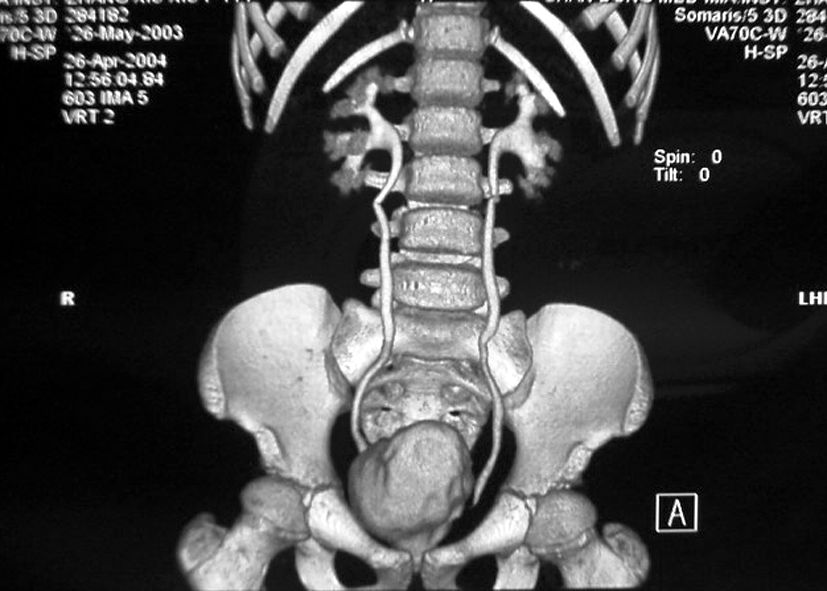
\includegraphics[width=.7\textwidth,height=\textheight,keepaspectratio]{./images/Image00316.jpg}
 \captionsetup{justification=centering}
 \caption{CT尿路成像}
 \label{fig15-1}
  \end{figure} 

\subsection{输尿管和膀胱的检查方法}

\subsubsection{输尿管检查}

①扫描前2h及0.5h各口服1.5%泛影葡胺500ml及300ml,以充盈小肠及结肠,必要时需通过直肠内注入造影剂。②扫描范围自耻骨联合下缘向上至肾门水平,层厚及层间距10mm;对较小的病变可加5mm以下的薄层扫描。③平扫是检出结石的主要方法。④增强扫描输尿管即显影,是输尿管肿瘤和先天性异常的理想检查方法。

\subsubsection{膀胱检查}

检查前准备同输尿管。膀胱肿瘤是CT检查的主要指征,膀胱壁的良好显示是正确诊断的关键。故需注意以下几点:①充分充盈膀胱,检查前1~2h让病人喝足量的水或阳性造影剂,既可充盈膀胱,亦可充盈小肠。②如膀胱内充入造影剂不宜过浓,否则不利于膀胱壁和小肿瘤的显示。③双重造影检查即向膀胱内注入CO\textsubscript{2}
或O\textsubscript{2}
100ml,同时注入2%的阳性造影剂或生理盐水200ml,利用体位改变(仰卧、俯卧)可充分显示膀胱壁和小肿瘤。

\section{正常解剖和变异}

\subsection{形态和大小}

1.位置:肾位于腹膜后,脊柱两旁。右肾比左肾低约1.5cm,左肾上端平T\textsubscript{11}
下缘,下端平L\textsubscript{2} 上缘;右肾上端平T\textsubscript{12}
,下端平L\textsubscript{3}
。偶尔左肾可低于右肾。儿童的肾脏比成人低,女子的肾位置一般比男子低半个椎体。两肾因受腰大肌向下、外侧斜行的影响亦向下、外侧倾斜。肾的内缘朝向内前方,外缘朝向外后方。但肾的位置并非固定,即立位和卧位不同。

2.形态:肾外形略似大豆,前面隆起、后面平坦、两端钝圆、外缘隆突、内缘中部凹入并裂开形成肾门。肾实质在肾门部围成的腔隙称为肾窦,容纳肾大小盏、脂肪组织及血管。肾门是肾盂和肾血管进出之处,进入肾门的结构称为肾蒂,其排列自前向后依次为肾静脉、肾动脉和肾盂。

正常成人肾脏表面光滑。婴儿肾表面有许多深沟称为肾裂,肾裂将肾分为10多个肾叶(图\ref{fig15-2})。肾裂1岁以后逐渐消失。

\begin{figure}[!htbp]
 \centering
 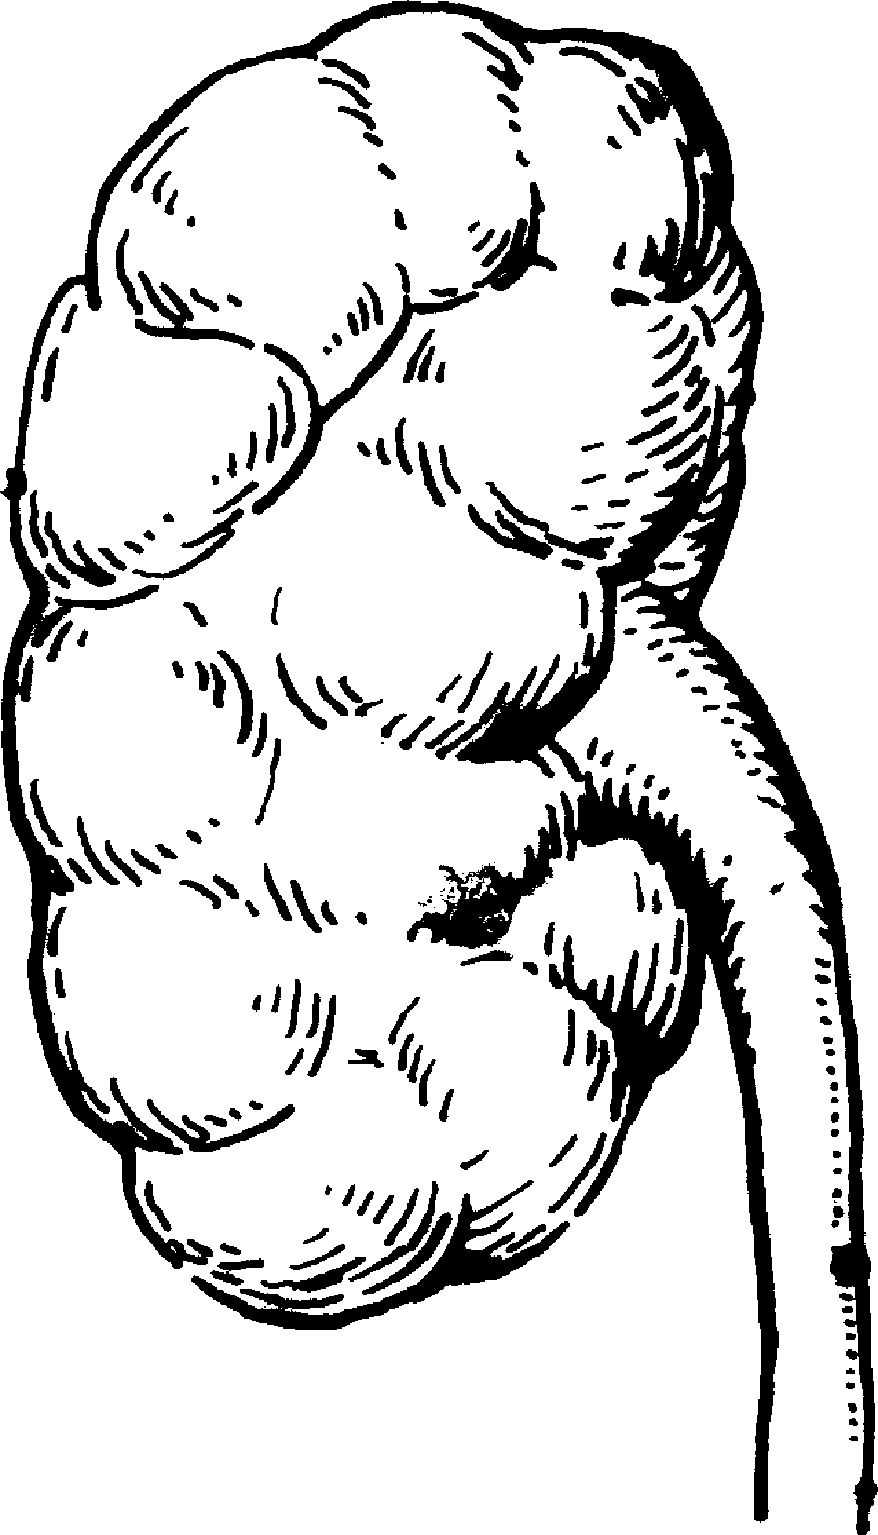
\includegraphics[width=.7\textwidth,height=\textheight,keepaspectratio]{./images/Image00317.jpg}
 \captionsetup{justification=centering}
 \caption{婴儿肾}
 \label{fig15-2}
  \end{figure} 

肾实质分为皮质和髓质两部分。肾的被膜由紧贴于肾实质表面的薄的纤维薄膜(固有包膜)、肾周脂肪囊和最外层的肾筋膜构成。

3.大小:成人肾长约10~15cm,宽约5~8cm,厚约3~4cm。一般左肾较右肾长1~1.5cm。

\subsection{正常肾实质的CT表现}

正常肾横断面呈圆形或椭圆形,可略有分叶,外缘光滑。肾的上下极较中部横截面积小。正常肾实质CT值为30~50Hu,稍低于脾。平扫时皮质和髓质密度一致,不能区分。

增强扫描肾实质的3相变化为:①血管显影期:即皮髓交界期。外周皮质和伸入髓质内的肾柱显影,密度升高,而髓质尚未显影,两者交界清晰。此期持续80~90秒。②实质期:即皮髓增强期。造影剂通过肾小管排泄,髓质显影,密度不断增高,最终与皮质密度一致或略超过肾皮质,皮髓质分界消失,CT值可达150Hu左右。此期持续1~2分钟。③肾盂排泄期:即肾收集系统充盈期。肾盂、肾盏及输尿管显影,肾实质密度降低。

\subsection{肾窦和肾血管的CT表现}

1.肾窦:肾门位于肾中部,右肾门较左肾门通常低1~2cm,也可出现在同一层面。肾门前中部有肾血管蒂和肾盂结构,深部为肾窦。肾窦内含有脂肪,与肾周脂肪密度相似。肾窦脂肪量多少不等,个体变异很大。如肾窦内脂肪少或无肾盂积水,平扫不能明确区分肾窦内结构。增强扫描肾盂肾盏显影,与不强化的肾窦内脂肪对比鲜明。

2.肾血管:平扫尤其是增强扫描可显示肾血管蒂位于肾盂前方,肾静脉位于肾动脉前方,口径较粗。多数肾动脉、静脉同层显示。①左肾静脉长于左肾动脉,在主动脉与肠系膜上动静脉之间穿越,最后汇入下腔静脉;②右肾动脉长于右肾静脉,行走于下腔静脉和右肾静脉后;右肾静脉斜向上汇入下腔静脉,故一般同一层面不能见到其全长;③两肾动脉进入肾之前均分叉,在肾窦脂肪内呈“Y”形表现。

两肾静脉或位于同一层面,或右侧较左侧低0.5~1.0cm。肾动脉显示率低于肾静脉。正常肾动脉粗0.5~0.7cm,起始部稍粗,管腔粗细均匀。正常肾静脉宽度<1.5cm,下腔静脉<2.7cm。

\subsection{肾筋膜及腹膜后腔的间隙}

肾筋膜:肾实质外有肾包膜,包膜外有脂肪,脂肪外有筋膜。前后肾筋膜在肾的外后方融合形成侧锥筋膜,再向前与壁层腹膜相连;在内侧与围绕大血管的脂肪融合。前后筋膜将腹膜后腔(是一个充满脂肪的间隙,上达横膈,向下一直延伸至盆腔)分为肾旁前、肾周和肾旁后3个腔隙。

1.肾旁前间隙:位于后腹膜与前肾筋膜之间。其内有胰腺、十二指肠和升降结肠,这些器官的病变可致前肾筋膜增厚,最常见的是胰腺炎和胰腺癌。

2.肾周间隙:又称“吉氏间隙”。位于肾前、后筋膜之间。前后筋膜向上融合附着于膈肌韧带(膈筋膜);侧方与侧锥筋膜融合;下方与髂筋膜和输尿管周围结缔组织有疏松连接。后肾筋膜在内侧与腰大肌、腰方肌融合。此间隙的下角向髂窝开放。肾周间隙的最弱点在下角内侧邻近输尿管,通过它尿和肾周渗液最易逸出。Kneeland等以尸检证明两侧肾周间隙可在下腔静脉前方跨中线相交通。

肾周间隙内有肾上腺、肾及血管、肾周脂肪以及肾集合系统近段。以上器官病变可伸及肾周间隙,使肾筋膜增厚、肾周脂肪消失。肾周脂肪内有时可见连接肾筋膜的条索组织(是由多种原因所致的连接组织增厚)。

3.肾旁后间隙:位于后肾筋膜及横筋膜之间,其中只有脂肪组织。此间隙向下开放达髂嵴,但在其内侧横筋膜与腰大肌筋膜融合,故阻断了左右肾旁后间隙的交通。腹膜后邻近结构的病变可累及肾旁后间隙。

\subsection{输尿管}

输尿管起始于肾盂沿腰大肌前方下行,在髂嵴水平以下,向外后斜行向下,于坐骨棘附近转向内侧,向前呈弧形进入膀胱。CT平扫不易显示或难以与血管区分;增强扫描横断面呈浓密的圆点状影,宽约5~7mm,沿固定的行径通过易于识别。积水扩张时呈水样低密度;增强扫描密度低于健侧,甚至形成液液平面。

1.输尿管的分段:①腹段:位于髂嵴连线以上,右侧越过右髂外动脉、左侧越过左髂总动脉进入盆腔。②盆段:位于髂嵴水平至膀胱,仍居腹膜后。男性与输精管交叉转向前内;女性在子宫颈外侧2cm处与子宫动脉交叉,转向其后内方达膀胱。③壁内段:斜行穿过膀胱壁,长约1.0~1.5cm。膀胱充盈时两输尿管口相距5~7cm,排空时相距可达2~3cm。

2.输尿管的狭窄:有3个,分别位于:①肾盂输尿管移行处;②越过小骨盆入口处;③穿过膀胱壁处。

3.输尿管壁的分层:由内向外分别为黏膜、肌层和外膜3层结构组成,其中肌层又有内纵、外环2层平滑肌。

\subsection{膀胱及其毗邻关系}

膀胱位于盆腔下部的前方,前缘接近耻骨联合。正常膀胱呈倒置的圆锥形,完全充满时呈圆形、卵圆形,边缘光滑整齐。膀胱容量约300~500ml,适度扩张壁厚<3mm。分为底、体、顶、颈4部分,各部分之间无明显界限。①顶部:在上,位置因膀胱充盈程度而异,顶部及后壁上方覆有腹膜;②体部:包括前壁、两侧壁及后壁;③颈部:位于前下方,尿道内口位于此处;④底部:呈三角形,朝向后下方。

膀胱三角:在膀胱底部,两侧输尿管开口与尿道内口组成的三角区称为膀胱三角。位置较固定。该区域无黏膜下层,其黏膜平滑无皱襞。

膀胱壁的分层:由内向外分别为黏膜层、平滑肌层和外膜层(由结缔组织形成)3层。

膀胱的毗邻关系:①膀胱的最下方至耻骨联合,耻骨后缘与膀胱前壁之间为耻骨后间隙。②在男性,膀胱底部下外侧邻接精囊;在精囊内方,膀胱底部与输精管壶腹为邻;膀胱颈与前列腺相邻。在女性,底部的后方借子宫膀胱间隙松散地附着于子宫颈及阴道前壁;膀胱颈则紧贴尿道周围肌肉和尿道。③成人膀胱颈稍低于耻骨联合上缘,女性可在耻骨下1/3水平,婴儿膀胱位置较成人高。④膀胱大小变化很大,在儿童上缘不应高于S\textsubscript{1}
水平,成人上缘不应超过S\textsubscript{2~3}
水平。⑤男性膀胱底部可被前列腺挤压;而无论男女,膀胱底部均可由提肛肌产生一压迹。⑥膀胱两侧面与提肛肌、闭孔内肌、壁层盆筋膜、膀胱前列腺静脉丛等相连。

\subsection{肾脏的正常变异}

1.肾驼峰状隆起

左肾上极外前方近脾侧可见三角形或驼峰状隆起。平扫和增强扫描驼峰状隆起部CT值与肾实质一致,增强扫描早期其皮髓质交界清晰,与正常肾实质一致。

2.胚胎分叶

新生儿肾表面可见各肾叶间的小沟,10岁左右各叶融合,表面皮质沟消失,部分肾叶不能完全融合而成为永存分叶,即胚胎分叶或小叶。CT表现肾脏大小正常,表面皮质沟正对正常肾柱,后者位于两个肾盏之间。

3.肾柱肥大

亦称Bertin柱增生。肾中部肾柱粗大突入肾窦内。在IVP时可将肾盏推开,易误为占位;CT平扫及增强扫描均与肾皮质等密度、皮髓质界限清晰(图\ref{fig15-3})。

\begin{figure}[!htbp]
 \centering
 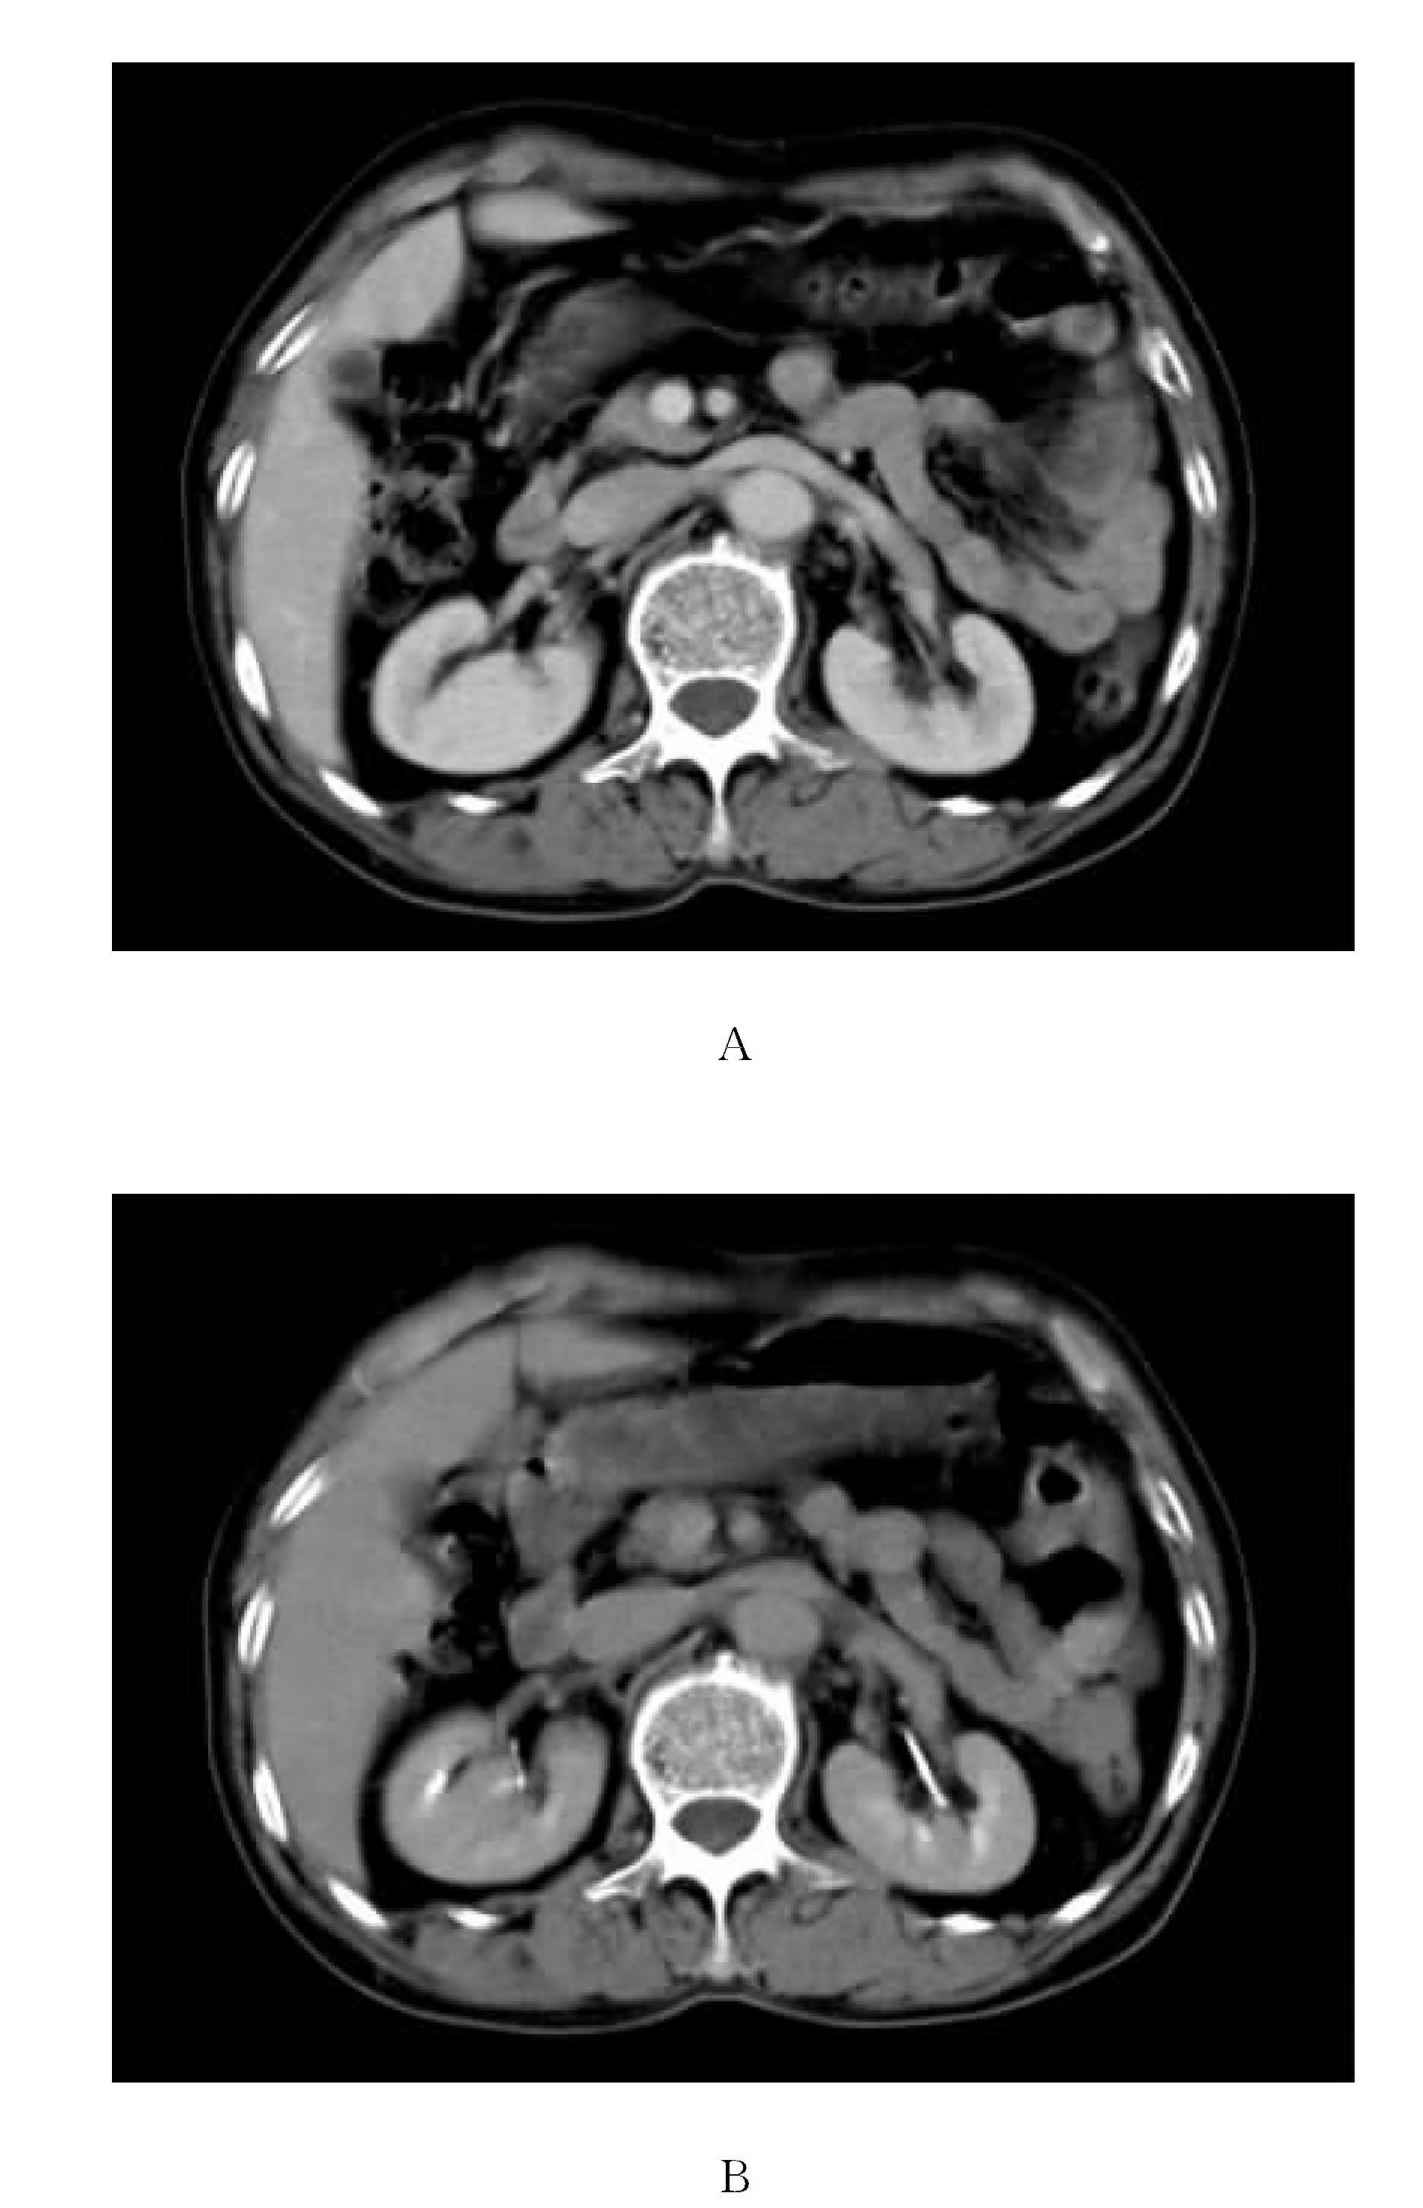
\includegraphics[width=.7\textwidth,height=\textheight,keepaspectratio]{./images/Image00318.jpg}
 \captionsetup{justification=centering}
 \caption{肾柱肥大\\{\small A为实质期,B为肾盂期;可见右侧有一肥大肾柱与正常肾皮质强化一致}}
 \label{fig15-3}
  \end{figure} 

4.肾窦脂肪增多症

又称肾窦脂肪异常增多。肾窦内脂肪含量变异大,与年龄、营养状况及某些肾病有关。肥胖、衰老和肾病所致的肾萎缩均可增加肾窦脂肪;另外,慢性肾盂肾炎、结石性肾盂肾炎、结核、动脉粥样硬化、缺血性疾病、创伤、梗塞也可造成肾窦脂肪增加。故可为正常变异,亦可为某些疾病所致。

本症是局限于肾盂、肾盏的改变,肾脏大小正常或稍小,其CT表现不同于肾血管平滑肌脂肪瘤和肾盂旁囊肿。

5.肾门血管变异

非常罕见,主要有:①环绕主动脉的左肾静脉:即左肾静脉离开肾门后分为前后两支,环绕腹主动脉,然后汇成一支入下腔静脉;②主动脉后左肾静脉。

6.肾外肾盂

肾外肾盂体积常较大,无论静脉肾盂造影、超声或CT均可能与轻中度肾积水混淆。但后者由于尿路阻塞、造成尿流量减少,少量高浓度造影剂沉积于下方,与尿液构成层状分界,这是肾积水的典型征象。偶尔肾外肾盂也有此征象,但无肾盏扩张。另外,肾盂的位置也是鉴别的依据。

但CT对排泄系统正常解剖的显示和轻度积水的检出不如尿路造影和超声,所以鉴别是困难的。

\section{泌尿系统先天性发育异常}

\subsection{孤立肾(肾缺如)}

先天性孤立肾即先天性单侧肾缺如,发生率为1/1000~1/1500。

\textbf{【病因病理】}
是一侧生肾组织及输尿管芽不发育,或仅存残缺的后肾组织所引起的。左侧发病较多,有家族患病倾向。70%可有其他泌尿、生殖系统畸形,其中最常见的是肾盂输尿管连接部狭窄。

\textbf{【临床表现】}
当孤立肾的功能正常时,不影响病人健康。多因出现并发症(如尿路感染或肾结石)或合并其他畸形而就诊。

\textbf{【CT表现】}
一侧肾窝内肾影缺如,被周围组织充填,其他部位也找不到正常或异常的肾脏。缺如肾的同侧肾上腺亦常相应缺如;8%~12%的肾上腺可存留,但呈长条状,而非正常的“人”或“Y”形。孤立肾的体积相对增大。

应注意与一侧肾发育不全、异位肾相鉴别。

\subsection{额外肾}

本病又称为附加肾。系独立存在的第三个肾脏,极为少见。

\textbf{【病因病理】}
它是一侧生肾组织分裂成两个,然后有分开的输尿管进入,而形成两个完全分离的有包膜的肾。额外肾有其独立的血供和输尿管。可并发输尿管口异常,合并感染、积水、下垂、结石的机会也较正常肾高。

\textbf{【临床表现】}
病人可无症状,但亦可并发肾积水、感染、结石或肿瘤而产生症状。常以发热、疼痛、尿路感染和腹部肿块而就诊。输尿管异位开口可形成尿失禁。

\textbf{【CT表现】}
可显示位于同一侧相互分离的肾和输尿管,对侧肾同时存在。额外肾较正常肾小,可位于正常肾的头或尾侧。

\subsection{融合肾}

融合肾为引起肾形态异常的常见原因。

\textbf{【病理及临床】}
①马蹄肾:即两侧肾上极或下极相融合。②盘状肾:即两侧肾的上下极均相互融合。③乙状肾:亦称人形肾。即一侧肾的上极与另一侧肾的下极相融合。④饼状肾:又称团状肾。即两肾在盆腔内近中线的广泛性融合,呈不规则分叶块状,通常上升仅达骶骨嵴水平,许多仍停留在盆腔内,两肾盂位于前方,两输尿管不交叉。

马蹄肾发生率为1/350~1/800,男多于女,是最常见的融合肾,且90%发生于下极。融合处为峡部,有异常供血动脉,同时伴旋转不良改变,往往伴输尿管畸形。一般无症状,多数因压迫神经、血管或输尿管而出现相应症状。

\textbf{【CT表现】}
CT能直接显示两肾融合的峡部或部位,以及朝前或前内的肾盂及肾门结构。CT很容易与肾先天性旋转异常相鉴别,而且能发现其所合并的结石、积水或肿瘤等合并症。

\subsection{异位肾}

\textbf{【病理】}
异位肾可位于盆腔、骶部、髂窝部等,高位异位肾可突入胸腔。如异位到对侧肾的下方,输尿管仍在原侧者,称为交叉异位肾或横过异位肾。异位肾多发育不全、外形小、有分叶等,并有旋转不良及输尿管长度异常。

\textbf{【临床表现】}
多无症状,但易并发感染与结石。常因触及“肿块”而就诊。

\textbf{【CT表现】}
一侧肾窝无肾影可见,可见异位至盆腔或对侧肾下方的肾脏,异位肾常有发育不良和旋转异常。异位肾合并的结石、积水或肿瘤可出现相应表现。异位肾位置固定,X线立位与卧位片可予显示。

\subsection{游离肾}

本病又称为游走肾。

\textbf{【病理】}
肾左右、上下活动度增大,超过正常范围,肾脏被异常的腹膜完全包裹。供血肾动脉都较长,常伴肾蒂或肠系膜的旋转不良。输尿管长度多正常,常在改变体位时折曲或被迷走血管压迫,从而产生不同程度的肾盂积水和继发感染。

\textbf{【临床表现】}
临床症状轻微,常有下坠感,久立明显。腹部可触及游动包块,可继发感染。

\textbf{【影像学表现】}
①仰卧位CT扫描表现左右肾位置正常,肾实质及肾盂肾盏多无异常表现;如有积水可出现相应表现;手法推移下扫描可见肾脏位置异常。②立位、卧位X线片或手法推移摄片比较可见肾脏活动度特别大。本病与位置固定的异位肾不同。

\textbf{【鉴别诊断】}
应注意与肾下垂鉴别。肾下垂多因随年龄增大韧带松弛所致,多无症状。CT检查价值不大,X线仅见肾脏上下移动,活动度>5cm。

\subsection{肾发育不全}

本病是肾脏在胚胎发育过程中生肾组织或后肾管发育障碍,以及血供不正常所致。多为一侧性,肾脏小于正常体积的50%以上。组织学表现肾单位数目减少,而肾单位及导管的分化和发育正常,肾小盏少于5个。

根据病理形态特点可分为3类。

\subsubsection{单纯性肾发育不全}

属非遗传性疾病,肾实质总量减少致肾体积小,但组织结构正常。一般为单侧。

临床上多见于女性,可无临床症状,或有高血压、结石、感染表现。

\textbf{【CT表现】}
一侧肾明显变小,肾实质变薄,而对侧代偿性肥大(图\ref{fig15-4})。但确诊需组织学检查。

\begin{figure}[!htbp]
 \centering
 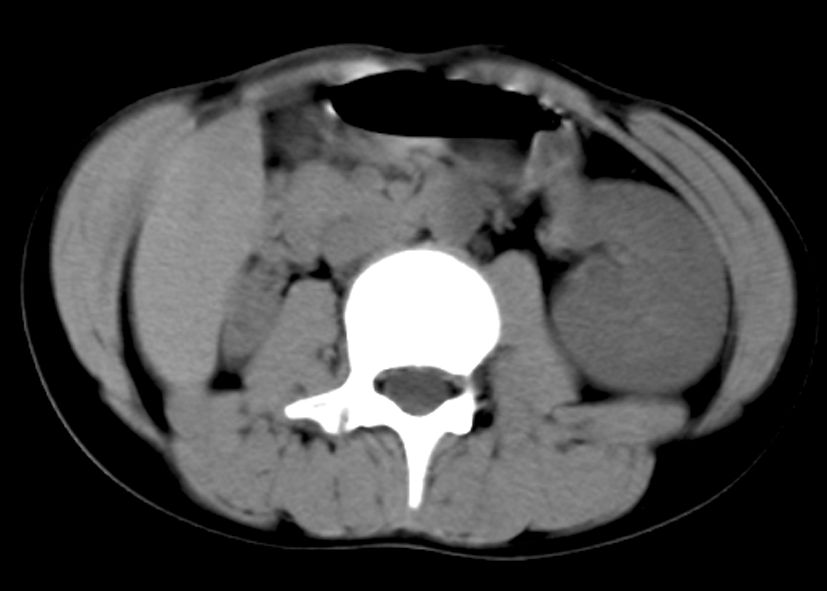
\includegraphics[width=.7\textwidth,height=\textheight,keepaspectratio]{./images/Image00319.jpg}
 \captionsetup{justification=centering}
 \caption{右肾发育不全\\{\small 右肾体积甚小,左肾代偿性增大}}
 \label{fig15-4}
  \end{figure} 

\subsubsection{节段性肾发育不全}

病理上肾实质部分变薄伴肾盏扩大,局部肾小管萎缩充满胶样管型,没有或仅有极少数肾小球,有时可见残留的髓质。

临床上多见于女性,有严重的高血压,50%有视网膜病变。

\textbf{【CT表现】}
患侧肾脏不规则萎缩,表面有切迹,肾实质厚薄不均;肾分泌功能明显减退。其CT表现与慢性肾盂肾炎无明显差异,需结合病史甚至活检鉴别。

\subsubsection{少而大的肾单位发育不全}

常为双侧性。病理特点为肾脏很小,肾小球数只有正常肾脏的20%,但肾小球显著肥大。晚期有间质纤维化和肾单位萎缩。

临床上患者呈进行性肾功能不全,通常于生后两年内出现症状,一般在12~15岁时死亡。

\textbf{【影像学表现】}
①CT表现肾脏变小,肾分泌功能减退。②逆行肾盂造影见肾脏变小,但肾盏并无畸形。

总之,肾发育不全尚无特征性CT诊断标准,需结合病史与慢性炎症、肾动脉狭窄引起的肾萎缩相鉴别。慢性肾盂肾炎所致的肾萎缩形态不规则,有瘢痕性切迹;肾动脉病变造成的肾萎缩血管造影显示不同类型的肾动脉狭窄,而肾发育不全时肾动脉显示细小。

\subsection{节段性肾发育不良}

本病又称为异形肾,是一种极为罕见的肾畸形。

\textbf{【病理】}
大体病理表现位于肾内的“肿块”多突向肾盂。“肿块”中的组织与正常肾脏组织结构一致,均有正常肾单位和肾小管结构。

\textbf{【临床表现】}
多无症状,可有腰痛,实验室检查多无异常。影像学易误诊为肿瘤。

\textbf{【CT表现】}
平扫肾区见略高密度或等密度肿块,肾盂、输尿管上端可有受压而积水扩张。增强扫描皮质期肿块边缘呈类似肾皮质样的环形强化,实质期呈均匀强化。双期甚至三期扫描肿块与正常肾实质强化的程度及时间-密度曲线一致,是本病的特征性表现,并以此与其他疾病相鉴别。

\subsection{输尿管重复畸形}

本病又称为重复肾,是一种常见的泌尿系发育畸形,大多发生于一侧,但也有两侧者。

\textbf{【病因病理】}
由胚胎期两个输尿管芽进入一个后肾胚基所造成。按输尿管芽分叉的高低引起部分重复或完全重复。多数肾实质仍融合为一体,表面可有一个浅沟,但肾盂多较小,发育不全。下肾盂较大,常有两个大肾盏。可以有一条或两条输尿管通向膀胱。如两条输尿管通向膀胱,一般上肾盂输尿管的管口开在下面。在男性输尿管下口可异位开口于尿道前列腺部、精囊、射精管或输精管(均在外括约肌近端,故均无尿失禁),在女性可异位开口于尿道、阴道或前庭(均在外括约肌远端,故可有尿失禁)。

\textbf{【临床表现】}
一般无症状,但下列情况可产生症状:①输尿管异位开口,尤其在女性可出现尿失禁;②常有尿液返流,易合并感染;③输尿管梗阻积水;④合并肾发育异常。

\textbf{【影像学表现】}
①IVP多表现为上肾盏萎缩变小或呈囊状;亦可有肾盂积水、输尿管迂曲,并可见异位开口。下肾盏近似正常,但肾盏数目减少、位置偏低。②CT见较正常肾的长径大(图\ref{fig15-5}),增强后可见双肾盂、双输尿管(但双肾盂不易显示),合并肾盂积水及肾肿瘤有相应表现。

\begin{figure}[!htbp]
 \centering
 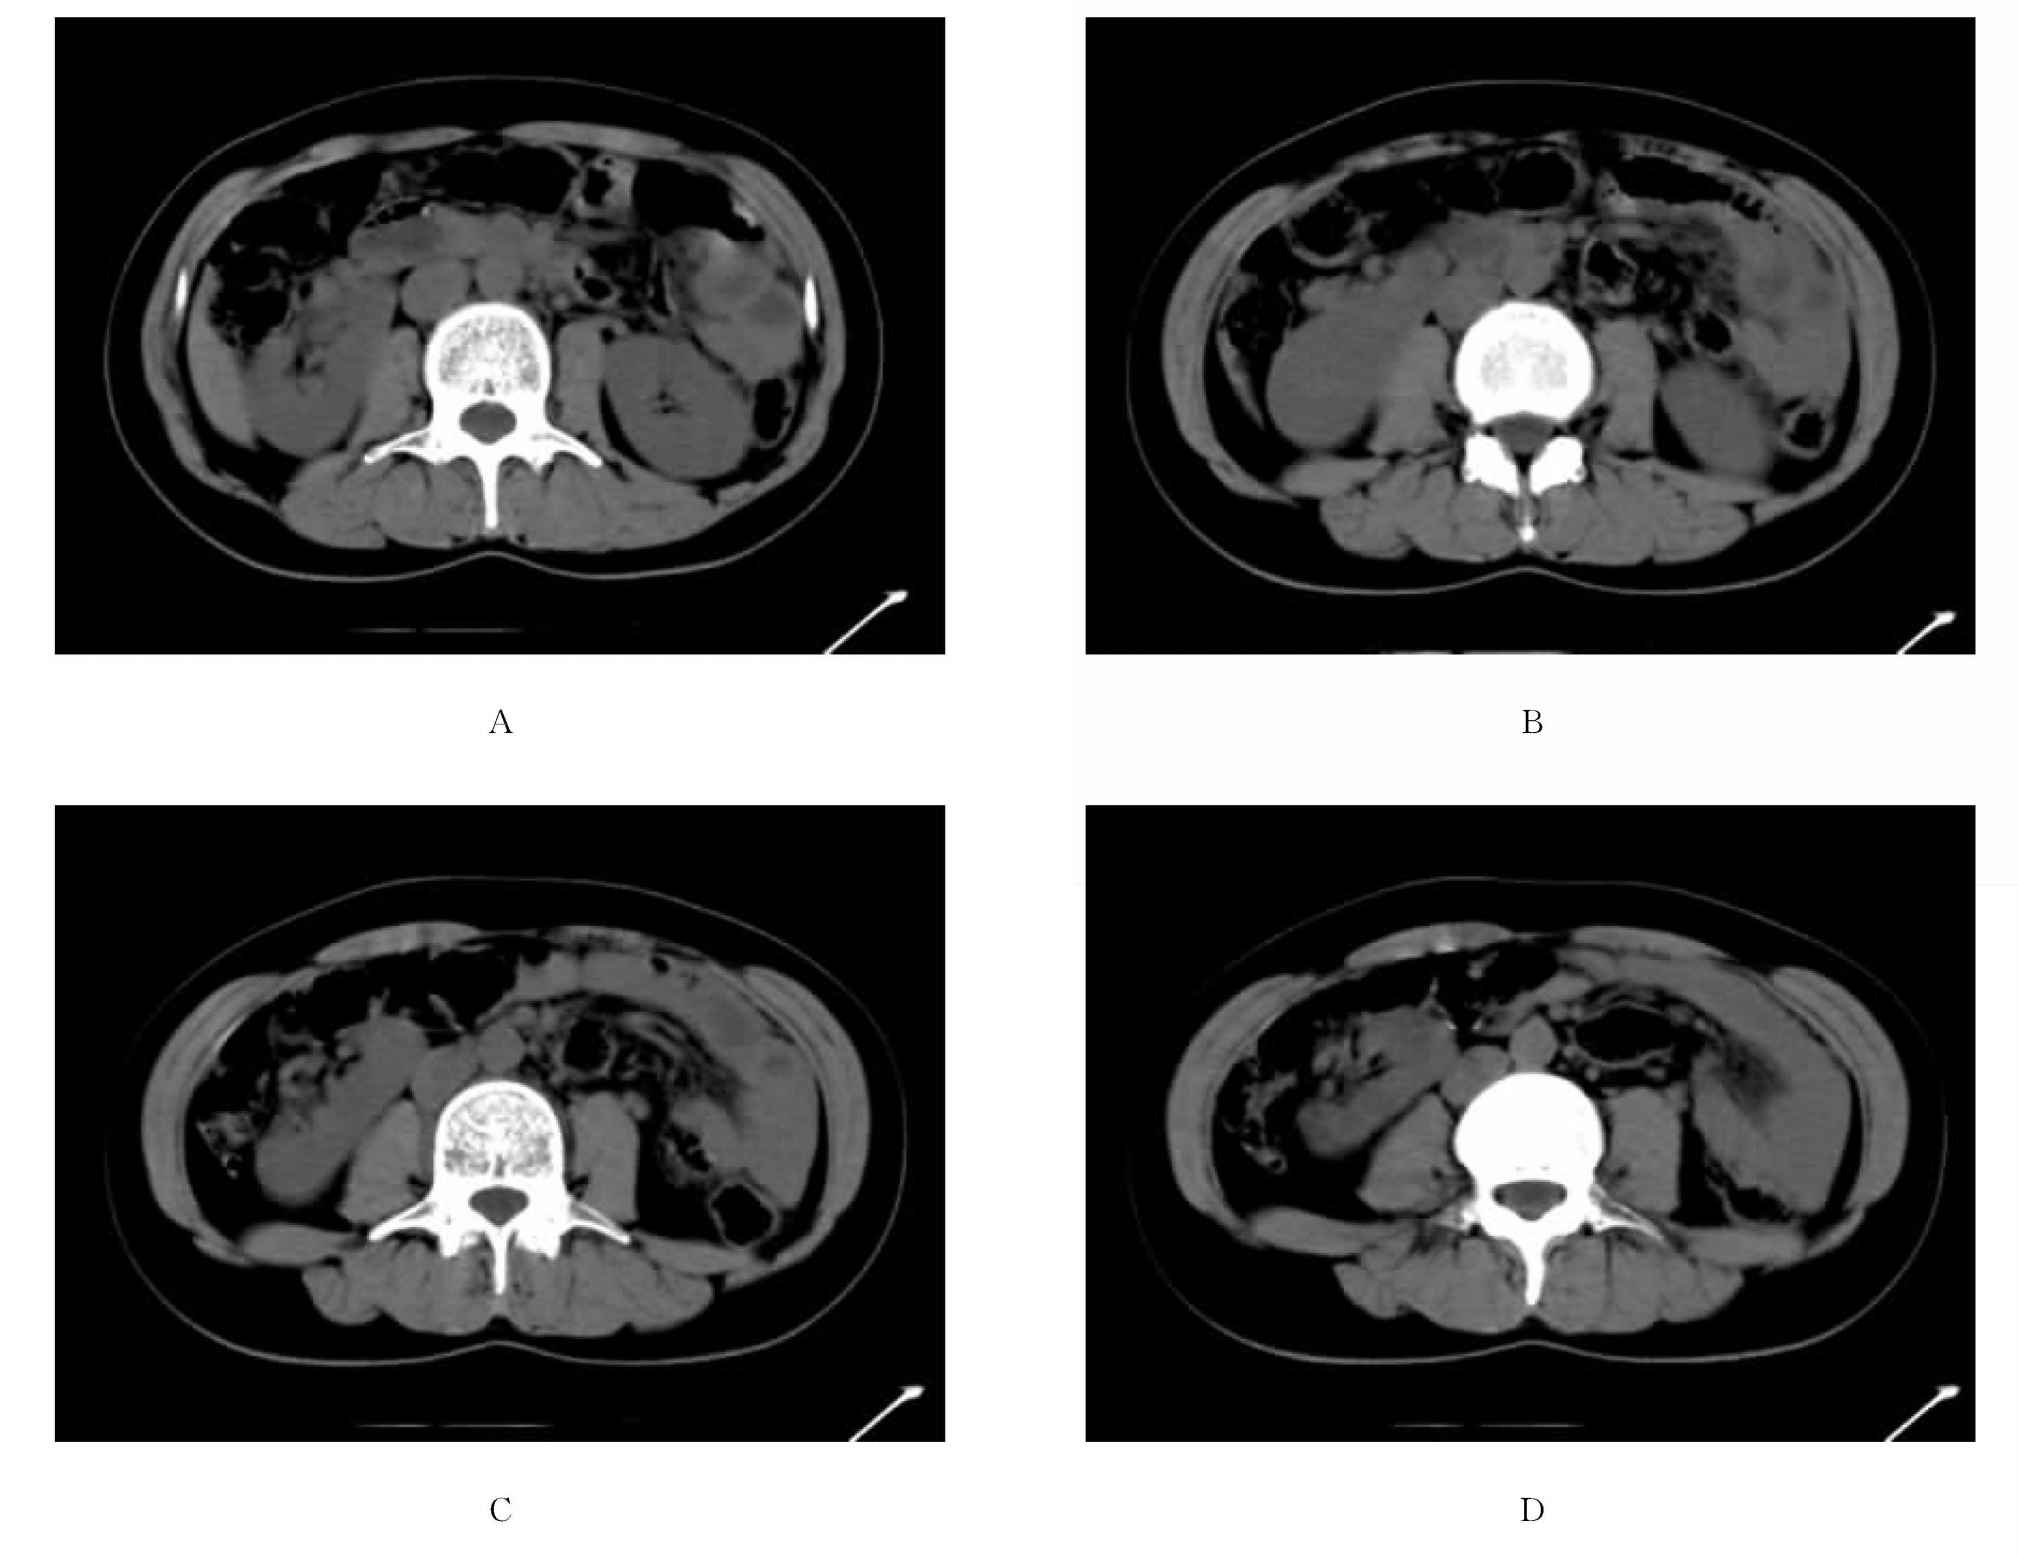
\includegraphics[width=.7\textwidth,height=\textheight,keepaspectratio]{./images/Image00320.jpg}
 \captionsetup{justification=centering}
 \caption{肾盂重复畸形\\{\small A~D为同一患者的上下连续图像,显示右侧有两个不连续的肾盂,且右肾旋转不良}}
 \label{fig15-5}
  \end{figure} 

影像学可分为以下4类:①双肾盂单输尿管;②双肾盂和部分双输尿管即“Y”型输尿管;③双肾盂双输尿管,下位肾盂输尿管开口在膀胱,上位肾盂的输尿管开口在其下方或为一盲端;④单一肾盂双输尿管。

\subsection{先天性输尿管狭窄}

本病大多位于肾盂输尿管交界处,是造成小儿、青少年肾积水的最常见的原因,以左侧发病为多。

\textbf{【病因病理】}
其病因尚不明,一般认为有两类。①机械性因素:包括先天性肾盂输尿管连接部环形肌肥大、异位血管及纤维索条压迫、输尿管肾盂开口过高,以及输尿管内瓣膜等。②神经性因素:由于肾盂输尿管连接部神经肌肉功能紊乱,交感神经过度刺激引起该处平滑肌持续性痉挛;肾盂无力或输尿管下端缺乏副交感神经节细胞使输尿管下端丧失蠕动等。

其病理学改变为狭窄段肌层肥厚、发育不良或纤维组织增生。

\textbf{【临床表现】}
多见于男性。常无明显症状,随病程延长,积水程度加重、肾实质变薄,最终导致肾实质的萎缩。就诊原因以腹部包块最多,可有腹痛、感染或血尿等。

\textbf{【CT表现】}
明确显示肾积水和输尿管扩张,可见扩张输尿管突然截断或变细处即狭窄段。如狭窄处未见高密度结石或软组织肿块,应首先考虑先天性输尿管狭窄,但CT难以显示狭窄段的形态,也不能对异位血管和纤维带压迫所致的肾积水做出病因诊断(图\ref{fig15-6})。螺旋CT尿路成像(CTU)可显示狭窄段的形态。

\begin{figure}[!htbp]
 \centering
 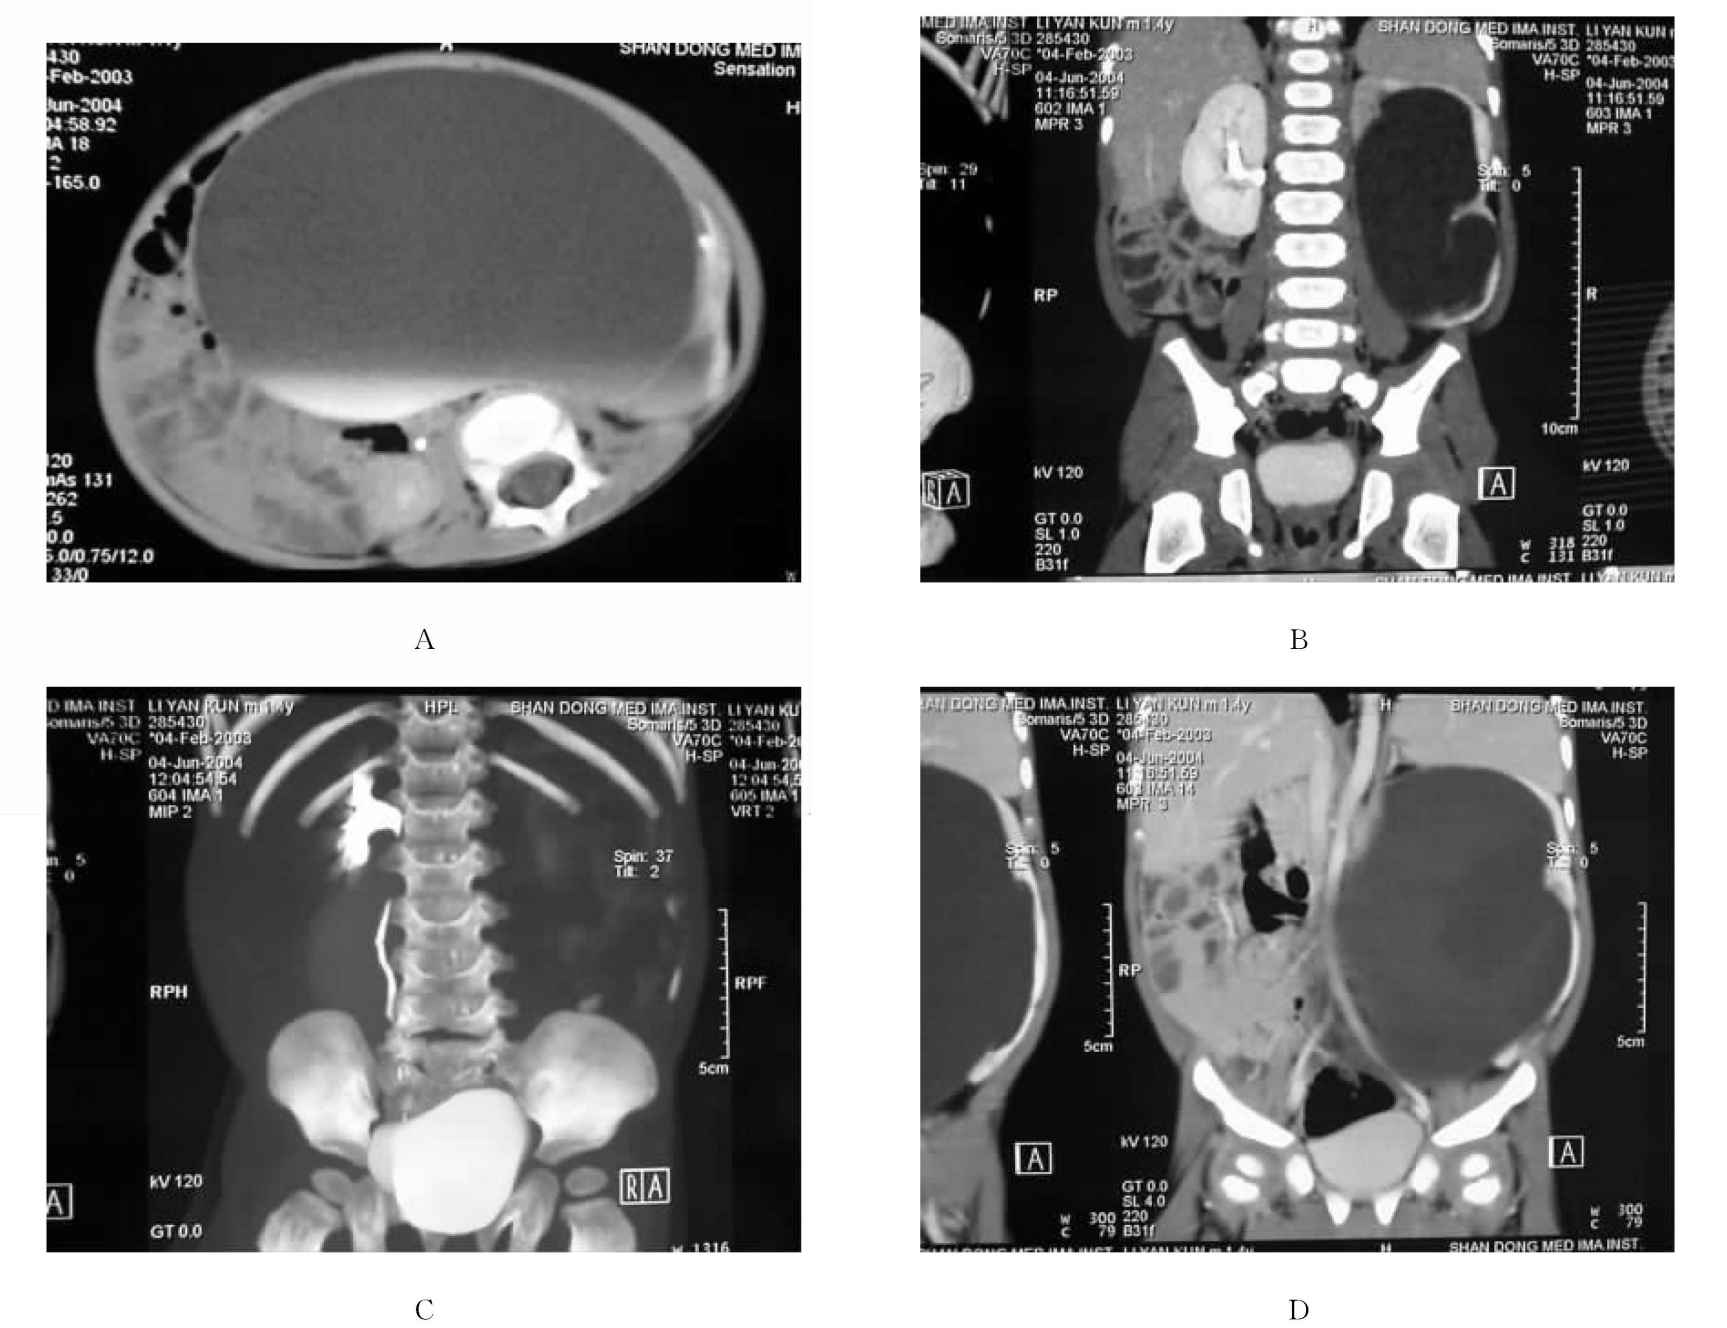
\includegraphics[width=.7\textwidth,height=\textheight,keepaspectratio]{./images/Image00321.jpg}
 \captionsetup{justification=centering}
 \caption{左侧先天性输尿管狭窄\\{\small A~D为同一患者,左肾积水呈巨大囊状水样密度灶,肾实质显著变薄}}
 \label{fig15-6}
  \end{figure} 

\subsection{输尿管囊肿}

本病又称为输尿管膨出,是输尿管口下端在膀胱黏膜下囊性扩张并突入膀胱。

\textbf{【病因病理】}
有多数人认为在胚胎期有生理性输尿管开口的狭窄或功能性挛缩,并致输尿管下端扩大形成囊肿;亦有人认为是膀胱壁内段输尿管过长或扭曲所致。病理见囊肿外层为膀胱黏膜,内层为输尿管黏膜,两层之间为菲薄的输尿管肌层。常为双侧性,且常伴有其他发育异常如输尿管重复、异位输尿管开口、输尿管先天性狭窄等。

\textbf{【临床表现】}
正位输尿管囊肿多见于成年女性;异位输尿管囊肿多见于女性婴幼儿。主要表现为尿路梗阻、膀胱刺激征和合并感染的症状。有时囊肿向尿道外脱垂。本病影像学诊断主要依靠膀胱镜、B超、IVU等。

\textbf{【CT表现】}
平扫呈大小不一的椭圆形低密度灶,边缘光滑。病灶位于膀胱轮廓线以内,常常以输尿管口为中心分布。囊内密度均匀,与膀胱内尿液呈等密度;囊壁厚度均匀一致,呈环形(图\ref{fig15-7})。如患侧肾功能正常,增强扫描可见囊内密度明显增高,且在较长时间内高于膀胱密度。如并发结石或输尿管积水等可出现相应表现。对异位输尿管开口,以CTU显示为佳。

\begin{figure}[!htbp]
 \centering
 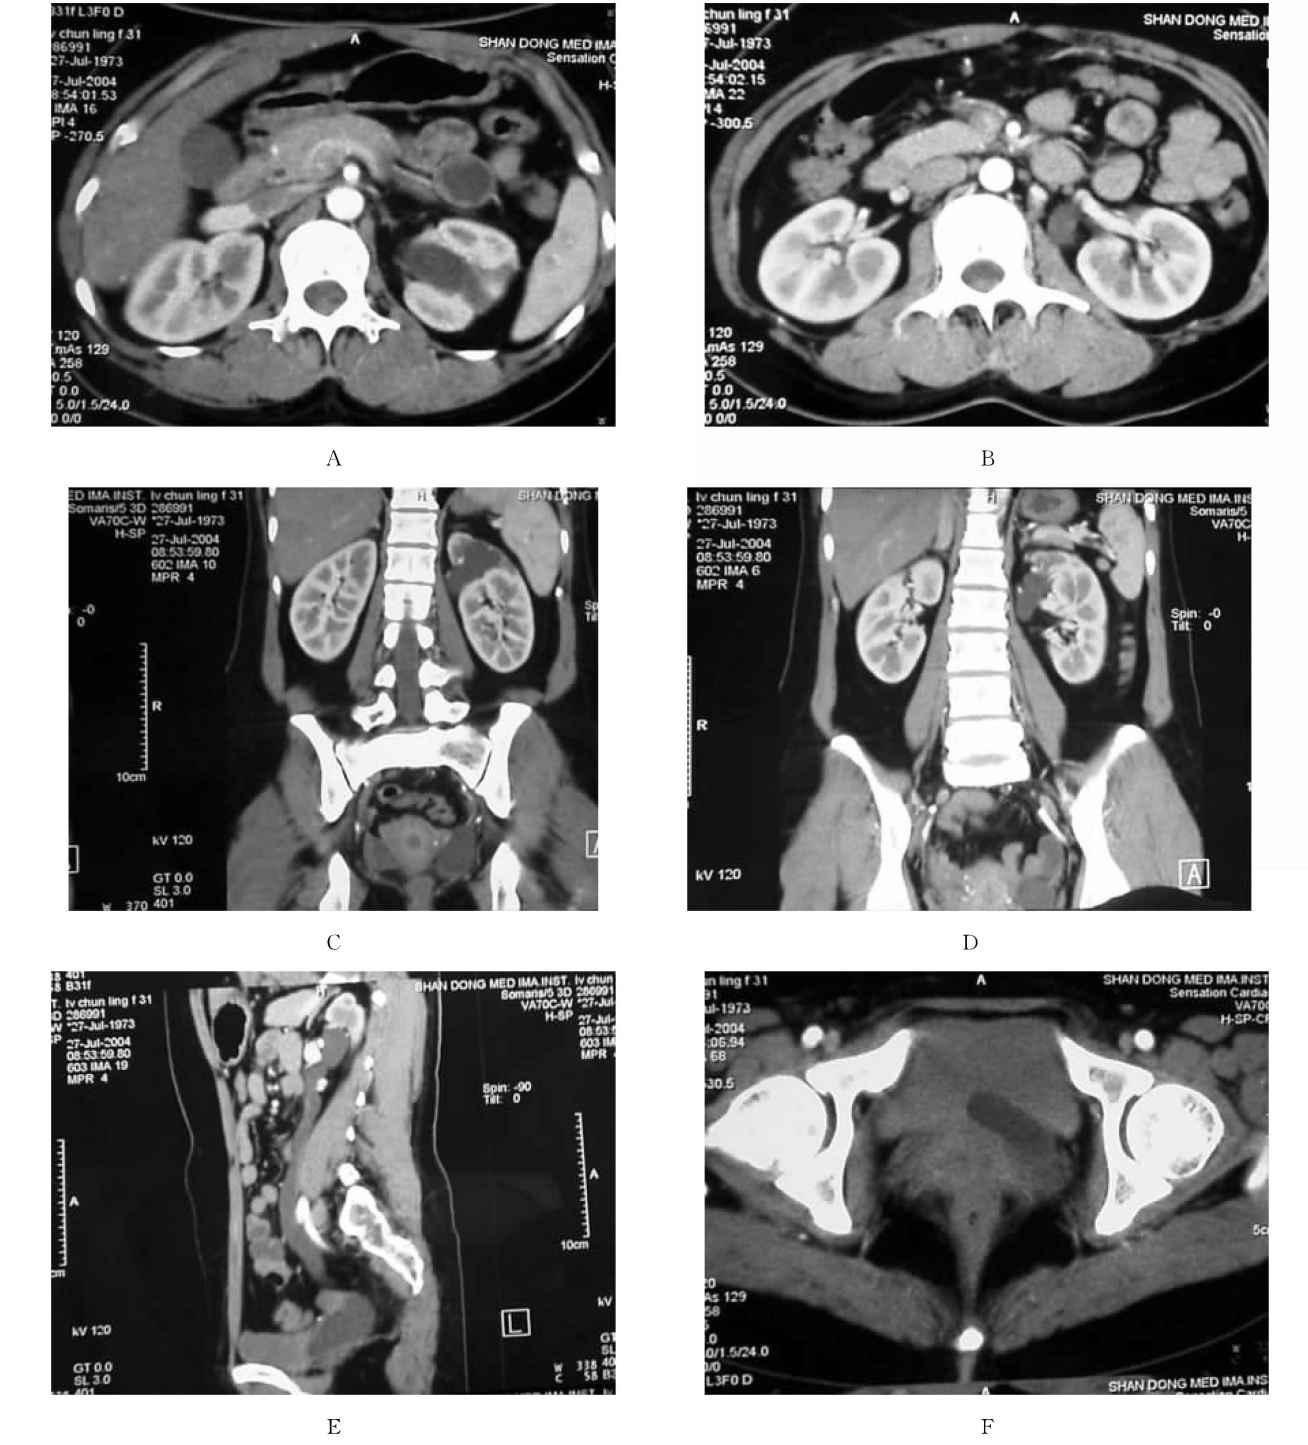
\includegraphics[width=.7\textwidth,height=\textheight,keepaspectratio]{./images/Image00322.jpg}
 \captionsetup{justification=centering}
 \caption{左侧重复肾并左侧输尿管囊肿\\{\small 左侧有两个分离的肾盂,左输尿管扩张,左输尿管下端呈椭圆形增粗,且突入膀胱}}
 \label{fig15-7}
  \end{figure} 

\subsection{先天性巨输尿管症}

此症系先天性输尿管扩张,整个输尿管显著扩张迂曲,直径可达4cm以上,可粗似肠管。

\textbf{【病因病理】}
一般认为本病是由于输尿管远端肌层弛缓性异常所致;也有人认为是由于输尿管肌层增厚、肌肉肥大所致,还有人认为是肌肉缺损引起;国外有学者发现输尿管末端缺乏纵行肌成分,完全由环形肌组成,从而造成功能性梗阻。总之,几乎所有学者都认为本病有输尿管远端的肌肉层异常,从而造成动力学失调。

有文献认为,组织学多可显示输尿管下段不同程度的肌性萎缩和壁内纤维化。严重病例病变段可全由纤维组织组成,而近段扩张的输尿管显示肌性外膜明显肥厚。

\textbf{【临床表现】}
有儿童型及成人型之分。前者病情发展较快,并发症较多,输尿管扩张程度较重,肾功能受损明显,多表现为尿路感染症状,也可出现血尿、腹痛、腰痛、腹部肿块、生长发育迟缓等症状;后者病情轻且相对稳定,主要症状为腰痛。

\textbf{【CT表现】}
可显示单侧或双侧肾积水及增粗扩张的输尿管,可粗似小肠,达4cm以上。CTU可提供更多的诊断依据。但与一些继发性巨输尿管无法鉴别或鉴别困难。X线造影检查还可显示邻近膀胱处的功能性梗阻段,长度为0.5~3cm、无缩窄;功能梗阻段无蠕动,其他段蠕动正常;扩张输尿管排空延迟,无膀胱输尿管返流。

\textbf{【鉴别诊断】}
本病与继发性巨输尿管不同,没有输尿管器质性梗阻、下尿路梗阻和神经源性膀胱,也无膀胱输尿管返流。

\subsection{下腔静脉后输尿管}

本病是下腔静脉发育异常中的一种先天性畸形,发生率约1/1000,多见于右侧,偶可双侧。

\textbf{【病因病理】}
本病是因外侧胚胎主静脉持续存在而引起。输尿管不在下腔静脉外侧,而是从下腔静脉后面绕行,然后再回到原来的走行路线上。绕行部位多在L\textsubscript{3~4}
水平,由于尿液通过此处多有障碍,因此其以上的肾、输尿管常有积水扩张。

\textbf{【临床表现】}
多见于男性,男性为女性的2~3倍。可无症状或表现为腰部酸痛,如并发感染和结石可出现相应症状。

\textbf{【CT表现】}
增强扫描可见输尿管在下腔静脉后方、内侧绕行,其上的输尿管有继发性积水扩张,如输尿管显影不佳则定位可能困难。

\subsection{膀胱先天发育异常}

\subsubsection{重复膀胱}

发病原因不详。分为完全性及不完全性,也可分为左右、前后和上下两个膀胱。此病多合并尿路畸形和下消化道重复畸形。①完全性:可见两个膀胱完全分开,同时有两个尿道;②不完全性:系膀胱内存在一个或几个不完全的分隔,使膀胱分成两个或多房膀胱。

应注意勿将巨大膀胱憩室误为双膀胱,巨大憩室总有一相对的狭颈相连,而突出于正常膀胱外,有助于鉴别。

\subsubsection{先天性膀胱缺如}

非常罕见。常伴有其他畸形,例如孤立肾、输尿管通于外部或直接与尿道连接。

\subsubsection{巨膀胱和小膀胱}

巨膀胱容积达数升,直至脐部,但无阻塞。小膀胱异常微小,仅容纳数毫升。

\subsubsection{膀胱外翻}

临床表现为腹壁不完全,膀胱无前壁而暴露于体外。X线可见耻骨联合分离。

\subsubsection{膀胱憩室}

或称真性憩室,是由于膀胱肌层的缺陷,形成膀胱的局部向外膨出。好发于膀胱的侧后部三角区上方,呈一袋形外突,有较小的颈部。

如为膀胱颈或尿道慢性梗阻时,膀胱内压力增高,促使膀胱壁在肌束间薄弱处突出而产生的憩室(假性憩室),常多发而小,界限不明显、底浅,应注意鉴别。此外,还应注意与卵巢囊肿、包裹性积液、精囊腺囊肿等相鉴别。

\subsection{脐尿管未闭和囊肿}

\textbf{【病因病理】}
脐尿管为胚胎期的尿囊管残余,在发育中应自行纤维化闭塞。如退化不全则脐尿管不闭合;如两端闭塞,则中间段管腔膨大、扩张,充满上皮层所分泌的液体而形成脐尿管囊肿。

\textbf{【临床表现】}
如脐尿管完全未闭时,在临床上可见到脐部有尿液排出。脐尿管未闭或囊肿合并感染则有腹痛、发热、局部压痛等,甚至引起腹膜炎和膀胱炎。

\textbf{【影像学表现】}

1.如脐尿管完全未闭时,于膀胱内或脐部注射造影剂,显示膀胱前上部与脐部相通,其下部一般较宽,脐部最窄。

2.如脐尿管一端闭塞,则余下的膀胱端或脐端成为盲管,造影剂仅见一端的残余管腔。

3.脐尿管囊肿:囊肿位于前下腹正中,可在肠道及膀胱上形成压迹。CT表现呈水样或实性密度,壁厚薄均匀。如合并感染其壁可均匀增厚,且壁强化显著。囊肿壁钙化为粗大钙化,且呈壳状。

\textbf{【鉴别诊断】}
本病需与卵黄管未闭鉴别,后者与肠道相通,因此排出物为粪便而非尿液。造影可见造影剂与肠腔相通,且都为下部回肠。

\section{泌尿系结石和积水}

\subsection{概述}

泌尿系结石的病因和形成条件及分类如下:

1.病因:①肾脏病变:如感染、细胞脱落、出血等;②尿路梗阻:导致无机盐沉淀;③代谢紊乱:如血钙降低、尿钙升高;④营养不良;⑤长期卧床。

2.条件:①中心核形成;②一定的黏着物质,是一种蛋白质;③结晶物质的沉积。

3.分类(根据结石的化学成分):①磷酸钙结石;②草酸钙结石;③磷酸镁胺结石;④胱氨酸结石;⑤尿酸结石;⑥尿酸盐结石;⑦碳酸钙结石。大部分为草酸钙和磷酸钙结石,其中草酸钙结石占全部结石的70%~80%。

\subsection{肾结石}

肾结石在泌尿系结石中居首位,单侧多见,10%为双侧性,80%位于肾盂内。

\textbf{【病理】}
结石可单发或多发。肾结石引起的病理改变主要是梗阻、积水、感染和黏膜损伤,导致上皮脱落、溃疡,最后纤维瘢痕形成。结石可与肾盂癌及感染同时发生。

\textbf{【临床表现】}
多见于20~50岁男性,腰痛和血尿是主要症状。其疼痛可为钝痛或绞痛。常向下部或会阴部放射。合并感染则出现尿频、尿急、尿痛和脓尿。

\textbf{【CT表现】}
国内文献认为无论何种肾结石在CT上均表现为高密度,且远远超过软组织密度,CT值约300~1300Hu不等(图\ref{fig15-8})。结石可呈层状、鹿角状、桑椹状、星状,亦可边缘光整。CT还可明确显示结石梗阻产生的积水、皮质萎缩和肾功能减退。

\begin{figure}[!htbp]
 \centering
 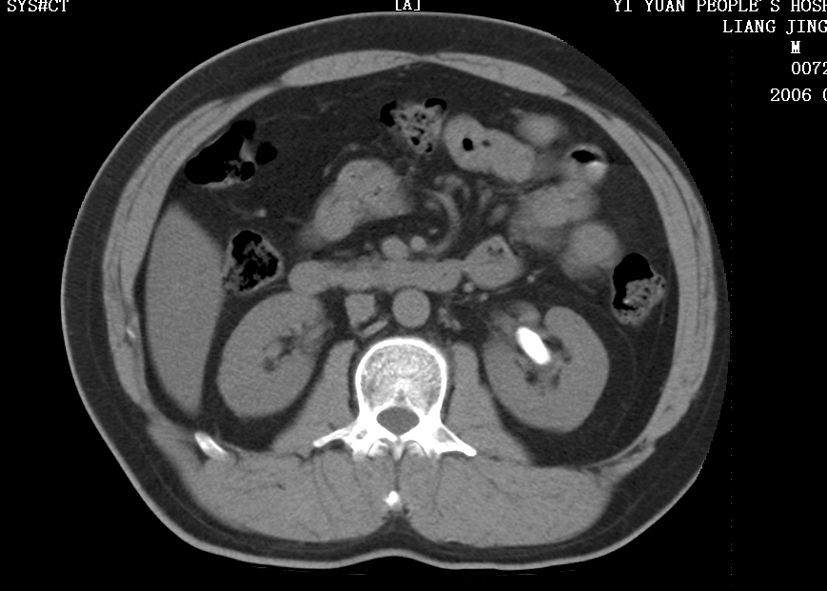
\includegraphics[width=.7\textwidth,height=\textheight,keepaspectratio]{./images/Image00323.jpg}
 \captionsetup{justification=centering}
 \caption{左肾结石}
 \label{fig15-8}
  \end{figure} 

\textbf{【鉴别诊断】}
应注意与肾钙化鉴别。广泛的肾实质钙化或钙质沉着症可见于高血钙、高尿钙、甲旁亢、髓样海绵肾、肾小管酸中毒、肾皮质坏死、肾乳头坏死、肾结核和高草酸盐尿。这些钙化分散且无肿块,与肿瘤不难鉴别,有时可与结石混淆。但钙化一般完全或大部分被肾实质包绕,而结石位居肾盂或肾盏区,多可鉴别。但收集小管(或称集合管)内结石与肾实质钙化难以鉴别,增强扫描借助扩张的收集管对鉴别有一定帮助。此外,结石和(或)钙化偶可位居肾轮廓外,其原因尚难以解释。肾内良、恶性肿瘤所致的局限性钙化常伴明显的软组织肿块,不难鉴别。

\subsection{肾钙乳}

肾引流系统内(多见于肾盏憩室、囊肿或肾盂积水内)有含钙质的混悬液存留者称为肾钙乳。

\textbf{【病因病理】}
本病病因尚不十分清楚,与肾内尿液的引流受障有关。国内报道肾结石与肾钙乳的关系密切,是由于肾结石引起梗阻和积水,给钙乳的形成创造了条件。从化学分析看,这种颗粒很小的钙乳其化学成分与肾结石基本一致,但为何不凝结成大的结石尚不明确,可能与某些物理因素有关。

\textbf{【临床表现】}
多无症状,一般以尿路感染、结石或肾积水等症状、体征而就诊。

\textbf{【影像学表现】}
肾钙乳的密度低于肾结石,CT值常在100Hu以上。因钙乳与积水相混合,故边缘不锐利,但个别囊肿型肾钙乳例外。钙乳呈团块或麻饼状,“麻点”密度较高,是由肾钙乳重叠所致。随体位变化形态和密度可变,显示钙乳液平有助于确诊。积水型钙乳,解除梗阻后钙乳量减少。

\subsection{输尿管结石}

输尿管结石一般由上尿路而来,原发者甚少见。

\textbf{【病理】}
输尿管结石引起的病理改变主要与阻塞有关。如阻塞时间较长则管壁变薄并有输尿管的伸长迂曲。有些梗阻以上的管壁肌层可以肥厚,还可发生结石周围的输尿管炎和输尿管周围炎。

\textbf{【临床表现】}
多见于20~50岁男性。主要表现为腰痛和血尿,多为绞痛和放射痛(向会阴部放射)。下端者可有尿频、尿急等症状,合并感染有膀胱刺激征。

\textbf{【CT表现】} 由于CT密度分辨力高,输尿管结石均可在CT上显示。

1.高密度的结石影:即在输尿管走行线路上呈现“钙化点”样高密度影(图\ref{fig15-9})。由于结石的阻塞,可见近端的输尿管和肾有积水扩张。有时可见肾周间隙、肾旁间隙及腹腔内少量至大量漏出之尿液及随之产生的炎性渗出液。

\begin{figure}[!htbp]
 \centering
 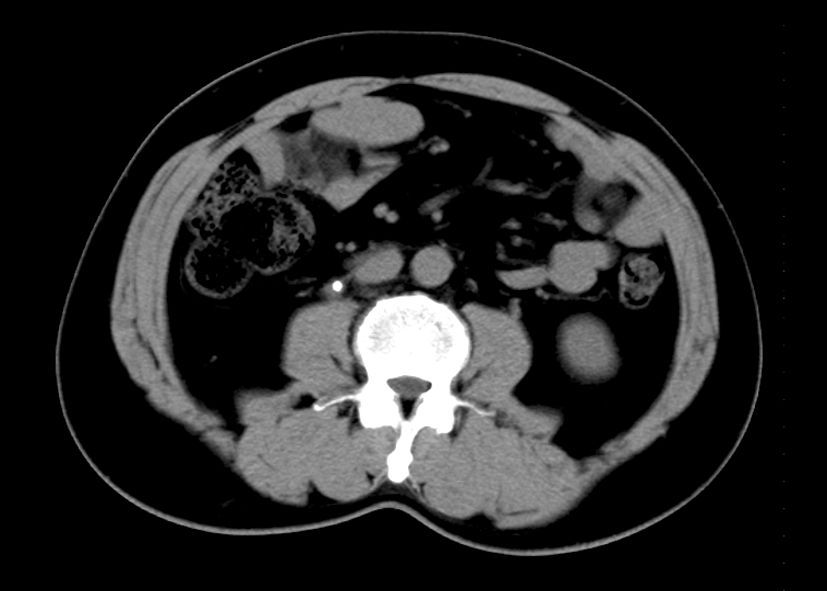
\includegraphics[width=.7\textwidth,height=\textheight,keepaspectratio]{./images/Image00324.jpg}
 \captionsetup{justification=centering}
 \caption{左侧输尿管结石}
 \label{fig15-9}
  \end{figure} 

2.轮缘征:又称组织环征,即结石周围的环状软组织密度影。其病理基础是结石嵌顿在输尿管内引起输尿管壁的水肿而形成。结石愈小轮缘征出现率愈高。较大的结石不出现轮缘征,是由于结石对输尿管壁过度扩张之故。但该征偶可见于静脉石和其他性质的钙化。

有时输尿管结石已走入膀胱,甚至排出,但仍可有肾盂、输尿管积水表现,应予注意。

\textbf{【鉴别诊断】}
盆内段输尿管结石应与盆腔静脉石相鉴别。其主要不同点如下:①国外有资料统计静脉石平均衰减值为160Hu(80~278Hu);而结石为305Hu(221~530Hu)。②静脉石常见中心透明和(或)一端对裂;而结石则无。③少数静脉石可出现彗星征(是由于血管搏动所致的放射状伪影);而结石则无。④静脉石所形成轮缘征是由于静脉壁不钙化所致,但出现率甚低。总之,平扫如无输尿管扩张,也无轮缘征显示,结石可能性不大。增强扫描更有助于鉴别。

\subsection{膀胱结石}

膀胱结石可由上尿路下降而来,或原发于膀胱内。

\textbf{【病理】}
膀胱结石大多来自肾和输尿管。原发结石的形成与尿滞留关系密切,炎性渗出物及膀胱内异物可组成结石的核心,经过尿盐的沉积形成结石。一般为单个,也可多发。此外,膀胱憩室内也可发生结石。

\textbf{【临床表现】}
主要见于男性,多为10岁以下儿童和老年人。主要症状是排尿困难、尿流中断、尿痛、尿频、尿急和血尿等。若结石位于膀胱憩室内,主要为继发膀胱感染的相应症状。

\textbf{【CT表现】}
膀胱内可见密度均匀或不均匀的圆形、椭圆形、同心圆形或桑椹形的致密影。多为单发,可小如绿豆,大如胎头,憩室结石可呈哑铃状。此外亦有报道,长期卧位者可出现膀胱钙乳。

\subsection{肾和输尿管积水}

\textbf{【病因】}
可分为梗阻性和非梗阻性两大类。①发生于肾盂输尿管交界处附近的梗阻:可见于先天性狭窄、异常血管压迫、结核、结石等。②发生于输尿管中部的梗阻:可见于结石、结核、下腔静脉后输尿管、肿瘤、游走肾等。③发生于输尿管下端的梗阻:可见于结石、结核、输尿管囊肿、肿瘤及手术后等。④非梗阻性积水:见于尿路感染、返流性肾炎、糖尿病等。

\textbf{【临床表现】}
病因不同而症状各异。腰痛最为常见,有时出现血尿。继发感染可有相应症状。

\textbf{【CT表现】}
①轻度肾积水:CT无阳性表现;②中度肾积水:显示肾盂、肾盏和(或)输尿管扩张(图\ref{fig15-10});与对侧肾比较,造影剂排泄延缓,肾实质密度下降;③重度和长期肾积水:肾影增大;增强扫描显示肾盂、肾盏明显扩张呈囊状或分叶状,肾皮质萎缩呈羊皮纸状;应注意与多囊肾相鉴别。

\begin{figure}[!htbp]
 \centering
 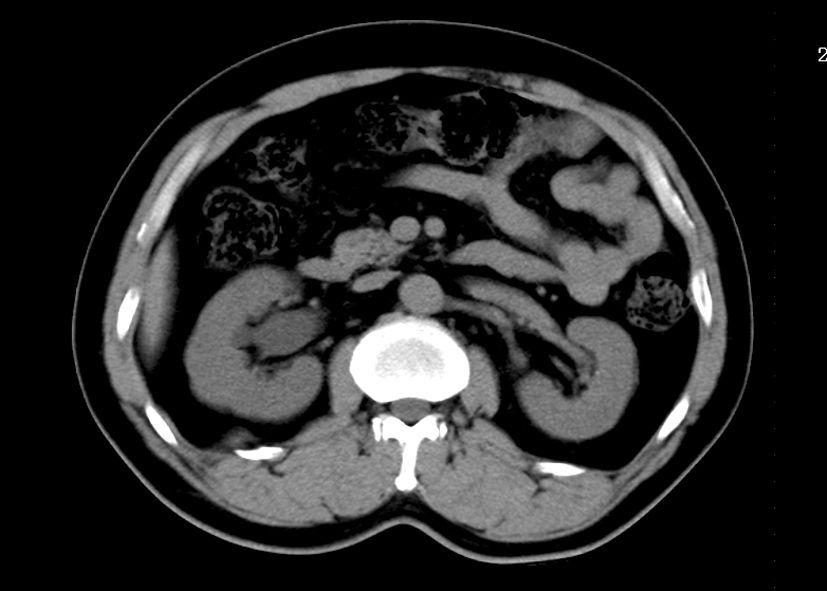
\includegraphics[width=.7\textwidth,height=\textheight,keepaspectratio]{./images/Image00325.jpg}
 \captionsetup{justification=centering}
 \caption{右肾积水\\{\small 右侧肾盂及部分肾盏扩张,呈水样密度}}
 \label{fig15-10}
  \end{figure} 

输尿管积水可见输尿管扩张,管壁可水肿增厚,也可管壁变薄、输尿管伸长迂曲。

\subsection{动力性尿路积水}

该病即非梗阻性尿路积水,是由于尿液积聚较多而排空相对较少所致,无尿路器质性阻塞,而仅有张力性减低或消失。

\textbf{【病因病理】}
病因有多种,如神经肌肉源性、先天性巨输尿管、中毒或炎症。此外,脊髓病变、肿瘤或外伤等引起的中枢神经异常改变亦为重要的病因。病理上以输尿管的改变最为明显,缺乏正常蠕动,若管径扩大明显时,则输尿管发生延长并扭曲,同时伴肾盂、肾盏积水。无输尿管器质性病变,亦无明显狭窄。长期积水易继发感染。

\textbf{【临床表现】}
主要因继发感染而出现尿频、尿急、尿痛和脓尿。也可出现肾功能损害的症状和检验指标异常。

\textbf{【影像学表现】}
可见肾分泌功能减退,肾盂、肾盏积水(图\ref{fig15-11})。两侧输尿管粗长迂曲,可甚似肠管,但在输尿管膀胱交界处无扩张。造影常可出现膀胱输尿管返流表现。

\begin{figure}[!htbp]
 \centering
 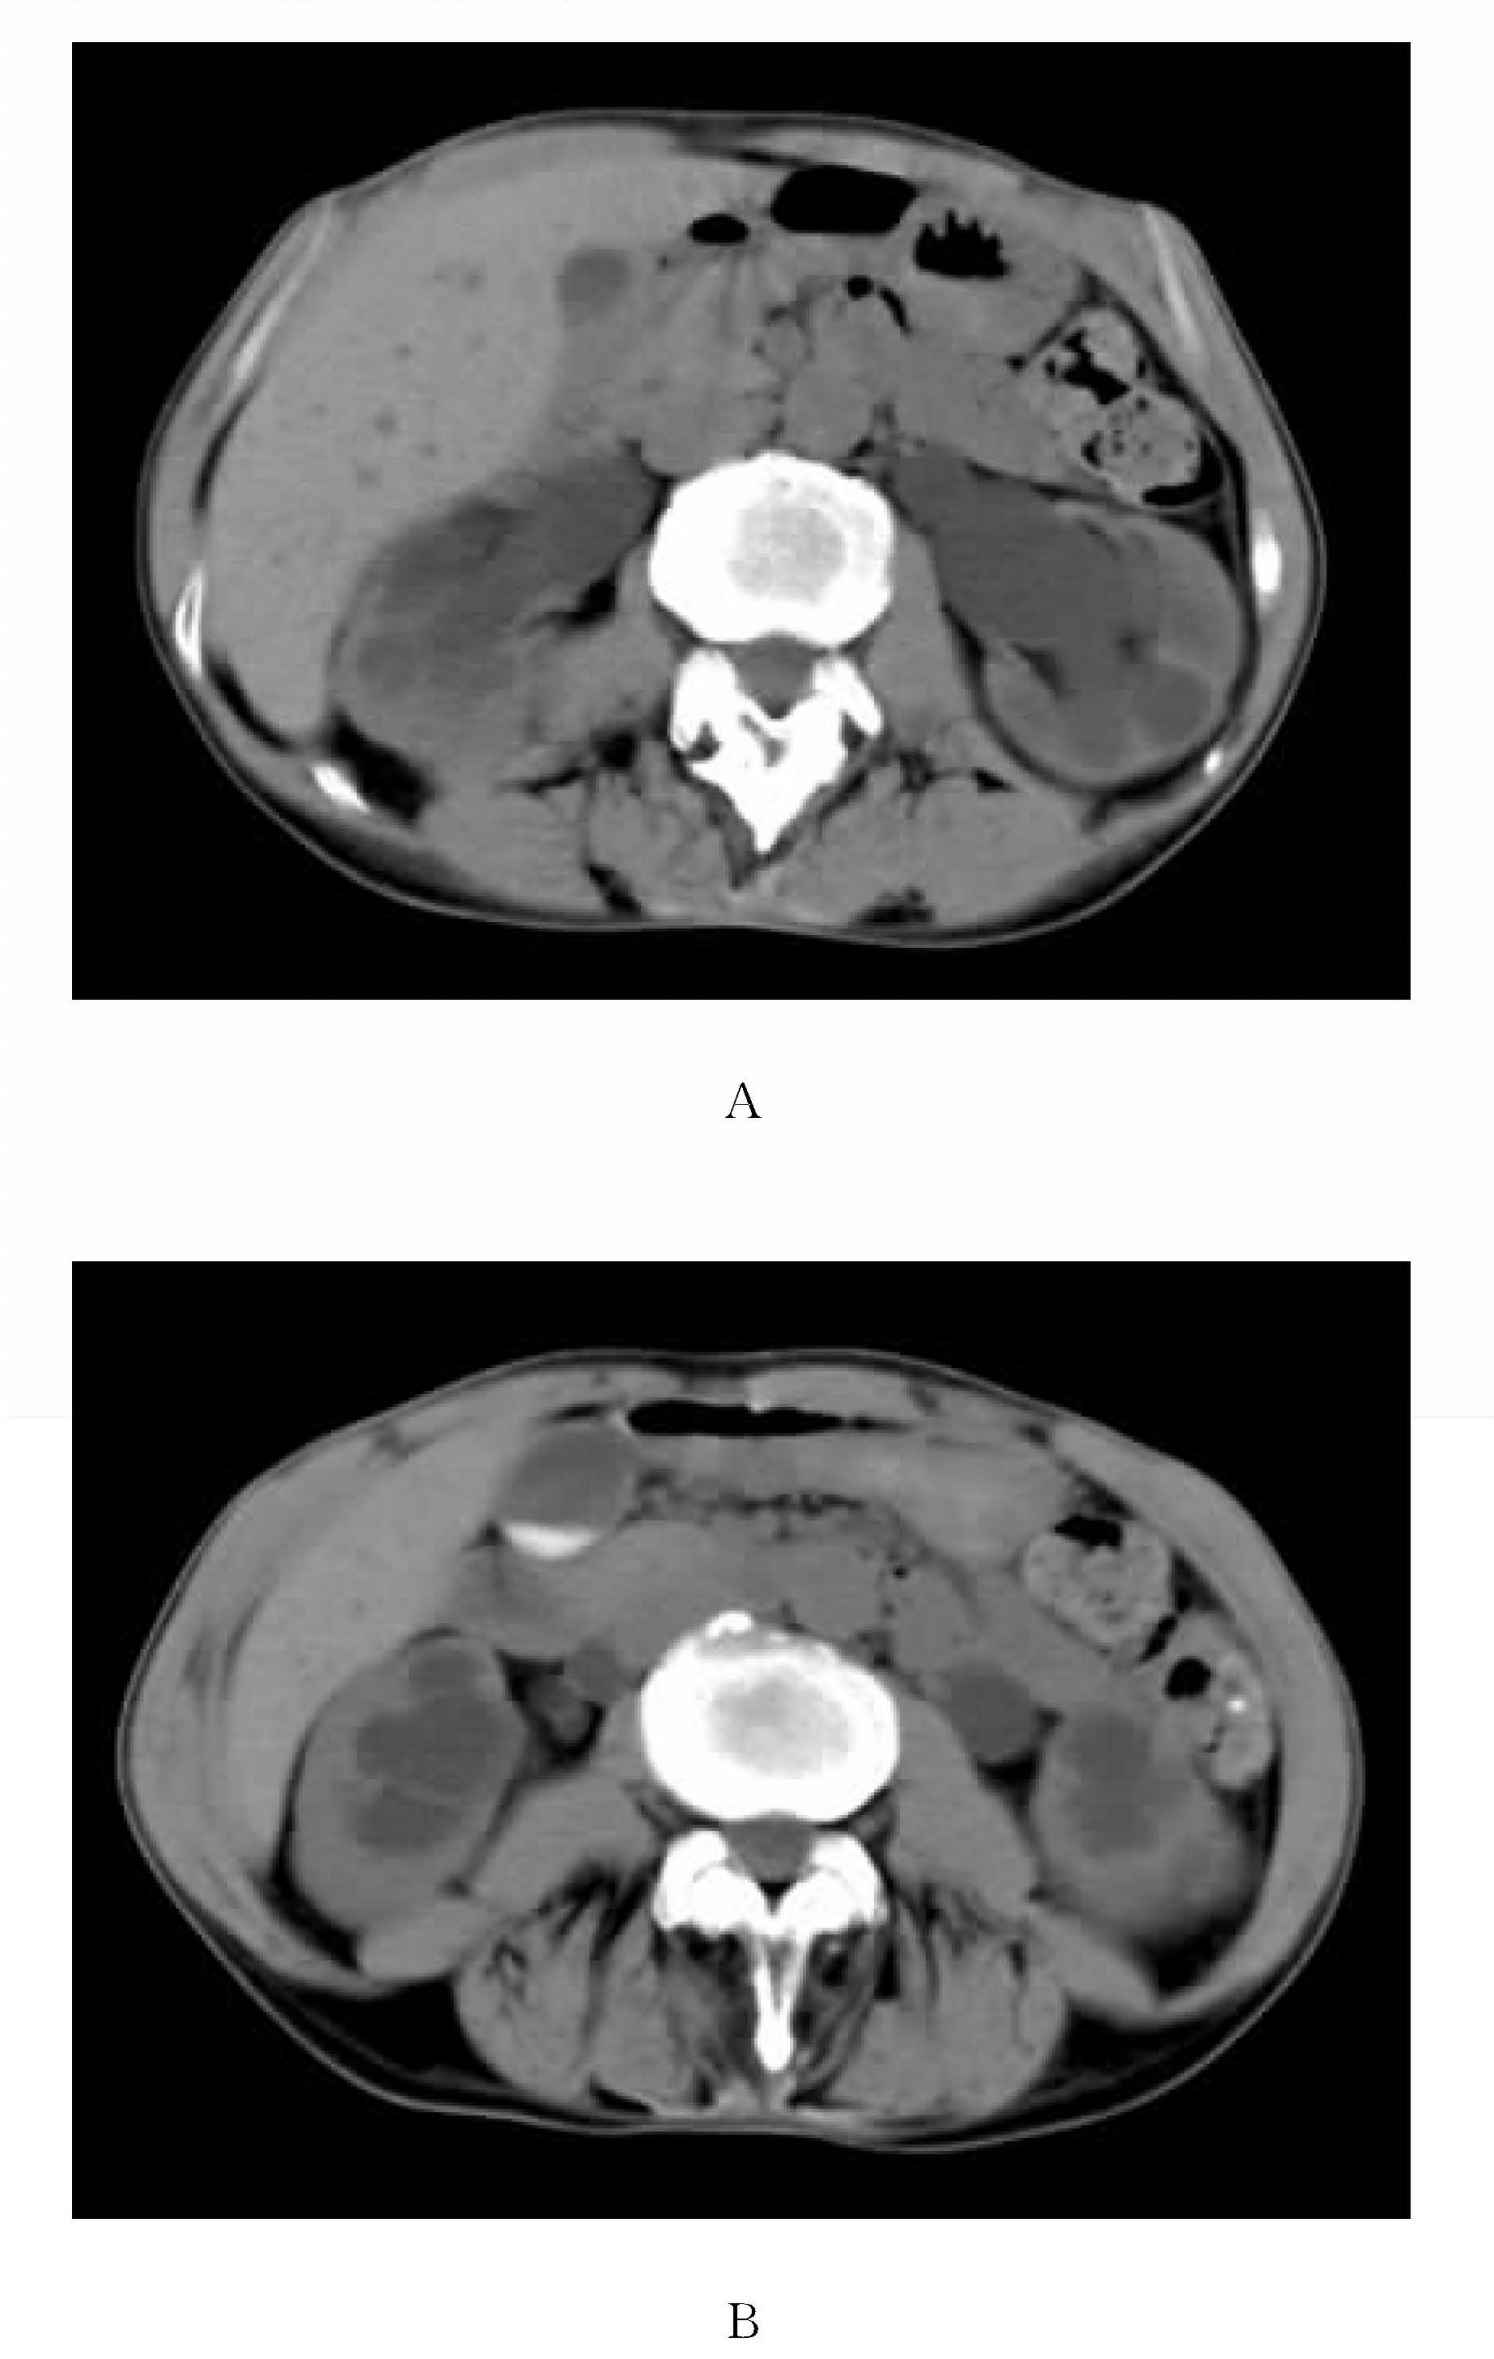
\includegraphics[width=.7\textwidth,height=\textheight,keepaspectratio]{./images/Image00326.jpg}
 \captionsetup{justification=centering}
 \caption{非梗阻性肾积水\\{\small 马尾神经损伤致大小便功能障碍7年。左右肾盂肾盏和输尿管上段均示积水扩张(胆囊内有泥沙样结石)}}
 \label{fig15-11}
  \end{figure} 

\subsection{神经性膀胱机能障碍}

本病又称为神经源性膀胱。膀胱的正常活动功能靠神经支配来完成。调节膀胱功能的中枢神经或周围神经受到损伤,致使膀胱的正常排尿反射阻断,而引起排尿功能紊乱,称为神经性膀胱机能障碍。

\textbf{【病因病理】}
常见于脑溢血、脑肿瘤、脑损伤、脊髓病变、隐性脊柱裂等。膀胱过度扩张或膀胱肌力长期增加均可形成憩室样改变。膀胱颈痉挛或松弛等可引起膀胱输尿管返流、输尿管及肾积水等改变,常并发感染及结石。

\textbf{【临床表现】}
常有不同程度的尿失禁、尿潴留和排尿困难。患者可因不同病因而出现不同症状,常有炎症和结石。

\textbf{【影像学表现】}
有不同程度的膀胱扩大,容量可达1000ml以上;膀胱壁边缘不规则,有很多内凹小梁,其间有多处向外凸出,形成大小不等的憩室;有时膀胱壁光滑。还可见膀胱颈松弛、痉挛,膀胱输尿管返流、输尿管及肾积水等表现。

但上述膀胱形态的改变亦可见于膀胱颈或颈以下的梗阻性疾病,需注意综合分析。

\subsection{输尿管夹层}

\textbf{【病因病理】}
直接原因是输尿管黏膜损伤和各种病理情况下导致的尿路梗阻。最常见的原因是结石的梗阻、肿瘤的梗阻或压迫、不同原因引起的慢性下尿路梗阻等。尿路梗阻后一方面导致肾血流明显减低,尿液生成减少,肾盂积水减慢,伴严重的肾功能损害。另一方面出现尿液的各种逆流和渗漏,其中以肾盂肾窦逆流最常见,且渗漏至肾外形成尿瘤。有学者认为,发生在输尿管中上段的渗漏则形成“输尿管夹层”,根据输尿管壁的解剖结构酷似主动脉夹层。总之,其形成的要素有:①肾盂输尿管黏膜损伤;②慢性输尿管梗阻;③肾功能良好。

\textbf{【临床表现】}
表现为腰痛和血尿等尿路梗阻的原发病症状,腰痛可向下部或会阴部放射。

\textbf{【CT表现】}
平扫可见输尿管呈“双环”及“双腔”改变,即“腔内腔”,真腔在内、假腔靠外,其内充满尿液。增强扫描早期假腔密度高于真腔,延迟扫描后则真腔密度高于假腔。真假腔的壁明显强化,夹层的上下端真假腔之间可见线条状粘连带。

\section{泌尿系感染性疾病}

\subsection{概述}

\subsubsection{病原菌及感染途径}

肾脏炎性病变为常见病。致病菌最常见的是革兰氏阴性杆菌,其中以大肠杆菌最常见,其次是副大肠杆菌、变形杆菌、克雷伯杆菌、产气杆菌、绿脓杆菌等。偶尔为革兰氏阳性菌如葡萄球菌、肠球菌及绿色链球菌等。肾结核亦非少见,真菌感染和病毒感染则比较少见。

肾感染的途径有:①上行感染;②血行感染;③淋巴道感染。以前两种多见。

\subsubsection{肾脏慢性炎症性病变的病因}

由于急性尿路感染的早期诊断和有效的抗生素治疗,肾慢性炎症不断减少。

其病因除人体抵抗力降低的因素外,其常见原因为膀胱输尿管返流、尿路梗阻、结石、糖尿病、先天性发育异常、痛风和滥用镇痛剂等。此外,急性炎症未能有效控制而反复发作也为原因之一。致病菌以大肠杆菌为主。肾结核和真菌感染一般作为肾脏的特异性炎症论述。

\subsubsection{反映肾脏炎性病变病理生理改变的CT表现}

1.肾轮廓的改变:①炎症急性期的隆起和肿胀;②慢性期的收缩凹陷。如一个轮廓不规则的小肾,往往见于慢性肾盂肾炎;而一个光滑的小肾,倾向于血供不足。

2.肾密度的改变:肾炎性病变在平扫时呈等密度或略低密度。增强扫描早期常无明显强化,而呈相对较明显的低密度;有文献报道,延迟期3h明显强化。病灶内气体是脓肿较可靠的依据。

3.肾功能的改变:①无功能肾可见于急性弥漫性肾盂肾炎的急性期、肾盂积脓、黄色肉芽肿性肾盂肾炎,以及慢性肾盂肾炎及肾结核晚期等终末期肾脏。②区域性肾功能减退可见于各种局灶性的急慢性炎性病变及肾梗死等。

4.肾周异常:肾急慢性炎症均可累及肾脂肪囊,造成肾周间隙积液和炎性肿块。而各类终末期肾脏、肾肿瘤和外伤等则可致肾包膜下及肾周血肿,肾癌、肾结核脂肪囊常清晰。

\subsubsection{肾脏急性炎症性病变延迟3小时扫描的诊断价值}

国内有文献述及对肾急性炎症性病变(除常见的大肠杆菌等细菌感染外,还包括真菌感染)延迟3小时扫描绝大多数在肾的炎性低密度区出现明显强化。可有3种表现形式:

1.平扫及增强早期密度不均匀的、带状的、楔形及马蹄形的低密度灶,延迟3小时与正常肾实质密度一致。此种表现最常见。

2.增强早期的低密度区边缘,延迟3小时呈局灶性或环形的明显强化。脓肿及肾盂肾炎伴空洞存在时,这肿表现几乎总能见到,有时可以见到早期未发现的小脓肿壁的强化。

3.表现为远离增强早期发现的局限性低密度灶的强化区,这种表现非常少见。有学者认为是由于血管痉挛造成远离病灶的局部缺血所致。

上述1、2两种表现可同时存在。造成上述延迟表现的原因是多方面的,但水肿导致的动脉血管床受压而引起的对比剂流入和流出的延迟是最可靠的原因。

\subsection{急性肾盂肾炎}

本病是肾脏的急性细菌性感染,根据炎症累及的范围可分为两型:①弥漫型;②局灶型。目前此病命名尚不统一,如急性细菌性肾炎和急性间质性肾炎;其局灶型又称为大叶性肾炎、急性局灶性细菌性肾炎和脓肿前期病变。

\textbf{【病理】}
病理上急性感染的致病菌开始均停留于肾髓质,然后波及皮质,病变可为局灶性、多发性和弥漫性。病变区间质水肿、炎性细胞浸润及微小脓肿形成,致肾局部或全肾增大。部分病灶内可有出血。

\textbf{【临床表现】}
好发于15~40岁的女性。起病急,可有发热、寒颤、尿频、尿急、脓尿、血尿、肾区叩痛及白细胞升高等,弥漫性急性期常伴可逆性的急性肾功能衰竭。如治疗及时炎症可完全吸收,否则可进展为肾脓肿。如反复感染半年以上,可演变为慢性肾盂肾炎。

\textbf{【CT表现】}

1.弥漫型:肾外形弥漫性增大,边缘不整齐。增强扫描肾强化减弱、皮髓交界时间延长、交界缘模糊;可出现单个或多个楔形低密度区;或1至数条条纹影,从髓质至皮质呈放射状分布。肾盂可轻度积水,肾周脂肪囊密度增高,肾筋膜增厚。

2.局灶型:平扫病灶呈楔形或圆形、单发或多发的等密度或略低密度,边缘不清;如伴新鲜出血,其内可见小斑点状致密影。增强扫描病灶无明显强化,而呈更明显的低密度,边缘趋向清晰。延迟3小时扫描病变区仍有功能,表现为较明显的强化,这一点有别于脓肿。

\textbf{【鉴别诊断】}

1.弥漫型:应与下列疾病相鉴别。①气肿性肾盂肾炎:为急性肾盂肾炎的特殊类型。CT鉴别的要点是肾盂、肾盏的破坏,以及弥漫性气体的存在,常蔓延至肾周间隙,鉴别不难。②化脓性肾盂肾炎:因肾盂或输尿管梗阻导致肾盂积水伴化脓性感染。CT示肾盂、肾盏的扩张,其CT值常>20Hu,高于一般积水;偶见少量气体。

2.局灶型:①肾梗塞:呈圆形或楔形低密度灶,通常较大者呈圆形,皮质缘可见侧支循环构成的环状强化带,有助于鉴别。但较小的病灶常呈楔形与局灶型很难鉴别,需密切结合临床和病史。②肾脓肿:呈圆形,病灶中央呈水样或略高于水的密度,增强扫描呈环状强化。③肾肿瘤:通常呈部分强化的实质性肿块,鉴别不难。但少数肿瘤可无强化而鉴别困难,需结合病史予以鉴别。

\subsection{气肿性肾盂肾炎}

本病是一种暴发性、坏死性的肾炎性病变,以肾实质内气体的产生为特征,常为单侧发病。

\textbf{【病因病理】}
好发于糖尿病、免疫机能低下、尿路化脓性梗阻、吸毒及长期慢性衰竭疾病的患者。致病菌常为大肠杆菌(68%),其次还有克雷伯杆菌,少数为厌氧菌。肾脏炎性缺血引起致病菌繁殖,使葡萄糖发酵成乳酸和CO\textsubscript{2}
,病变组织常明显坏死。

\textbf{【临床表现】}
病人除发热、寒颤、尿频、尿急、脓尿、血尿、肾区叩痛及白细胞升高等表现外,多有严重的败血症,死亡率高达50%。常有糖尿病、尿路梗阻和免疫抑制剂治疗史。

\textbf{【CT表现】}
主要为肾外形增大,可有轻度积水表现;肾实质多处破坏;肾功能明显减退或丧失。肾内及肾周弥漫性气体与低密度软组织影合并存在、肾筋膜增厚是其特征性表现。肾内可见多个含气脓腔,甚至有液平面表现。气体可扩散至邻近脏器;气体吸收较慢。

\subsection{化脓性肾盂肾炎}

本病亦称为肾盂积脓或脓肾,是由于肾盂或输尿管上段梗阻所引起的肾盂化脓性感染。

\textbf{【病因病理】}
梗阻原因可为结石、先天性狭窄、肿瘤等,主要为结石。梗阻引起肾盂、肾盏积水扩张,继而引起感染化脓。主要致病菌为大肠杆菌。

\textbf{【临床表现】}
常见于妇女、有糖尿病史及以往有尿路感染史患者。病人最初有发热、败血症和脊肋痛。实验室检查有白细胞升高、脓尿和细菌尿。

\textbf{【CT表现】}
肾外形增大,增前扫描肾功能明显减退或丧失。肾盂肾盏扩张积水,CT值>20Hu,密度欠均,可有少量气体。还可显示肾盂或输尿管存在的结石、狭窄等阻塞因素。

\textbf{【鉴别诊断】}
本病与急性肾盂肾炎和气肿性肾盂肾炎均可有肾盂积水表现。但急性肾盂肾炎积水程度轻,液体CT值低且无气体存在,肾功能损害轻;气肿性肾盂肾炎病程短,肾实质破坏伴气体的弥漫性存在是其特征性的CT表现,临床上常有糖尿病和免疫抑制剂治疗等病史。

\subsection{肾脓肿}

本病为肾实质内局灶性炎症液化坏死所致的脓液积聚。逆行感染是主要的感染途径,少数可由血行播散引起,但也有文献认为以血行感染为主。

\textbf{【病理】}
肾脏因充血水肿而胀大。多数为小的化脓灶分布于皮质和(或)髓质,小的脓肿逐渐合并成较大的脓肿。约1/3~1/2肾脓肿的感染蔓延至肾被膜并侵及肾周和肾旁间隙,形成局部炎症或脓肿。

\textbf{【临床表现】}
起病急,常有发热、脓尿、菌尿、脓毒血症、肾区疼痛和叩痛。如未能有效控制转成慢性肾脓肿,则临床症状常不明显,常无脓尿或菌尿,但可有低热、贫血和体重下降。偶尔急性期亦可无脓尿和菌尿。

\textbf{【CT表现】}
①脓肿早期和前期:即局灶性炎症期,呈前述的炎症表现。②脓肿成熟期:即急性期肾脓肿,平扫呈圆形低密度灶,边缘欠清晰,密度均匀。增强扫描呈厚度均匀的环状强化带,中央无强化,周围有低密度水肿带。③慢性期脓肿:病灶边缘清晰,中央明显液化呈水样密度。增强扫描呈周围宽窄不等的环状强化带,有时可呈典型的同心圆征。

肾脓肿的其他CT表现有:①病灶蔓延至肾周及肾旁间隙,致肾周间隙模糊或消失,肾筋膜增厚。并可形成肾周及肾旁脓肿,甚至形成腹壁和腰大肌脓肿。②无论肾内、肾周或肾旁脓肿,少数可见脓肿内的少量气体;偶可出现液平面,为脓肿的典型表现。③愈合期因纤维瘢痕收缩而致肾轮廓的凹陷变形。

\textbf{【鉴别诊断】}

1.肾癌:典型肾癌与脓肿不难鉴别,但下列情况可以混淆:①肾癌坏死液化或囊性肾癌:一般而言,肿瘤坏死灶密度很不均匀,内壁不规则,而慢性脓肿壁较规则;肾癌的肾周侵犯较局限,而脓肿趋向于蔓延;肾癌的强化持续时间短,而脓肿则较长。如见到肾静脉侵犯、癌栓形成或局部淋巴结增大,则支持肾癌。②少血管性肾癌:与脓肿早期一样,均呈低密度占位,强化不明显或轻度强化,两者有时鉴别困难。病灶强化时间的长短,可作为参考依据,密切结合临床甚为重要。

2.肾囊肿继发感染:囊肿壁增厚,密度增高,可类似于脓肿。但囊肿壁较完整,无环状强化带,必要时随访观察。

\subsection{慢性肾盂肾炎}

\textbf{【病因病理】}
可分为3个类型:①返流性;②梗阻性;③特发性。本病除慢性间质性肾炎改变外,还有肾盏、肾盂炎症,纤维化变形,且在临床及细菌学上应有肾感染的证据。病变涉及肾间质、肾小管和肾小球。不规则分布的纤维化瘢痕伴残留的肾组织增生导致肾脏萎缩和变形。

\textbf{【临床表现】}
多见于年轻女性。大多无明显尿路感染的症状,尿液检查正常,且一般情况良好,直至肾衰才出现相应症状,如乏力、纳差、体重减轻、头晕、头痛、恶心、呕吐和贫血等尿毒症症状。伴尿路结石可有腰痛、血尿等症状。

\textbf{【CT表现】}
①可无明显异常;②肾外形可有粗糙的皮质瘢痕;③肾乳头收缩和肾盏扩张、变钝;④严重者患肾萎缩变小;⑤肾盂轻度扩张积水;⑥增强扫描肾内瘢痕与萎缩凹陷的皮质缘相连,瘢痕内残存的肾组织增生呈“假肿瘤状”,肾功能有不同程度减退。

总之,病变可累及一侧或两侧肾脏,有时仅累及肾脏的一部分,通常为上极或下极。局部皮质变薄以及相应的肾盏扩大为本病的特征性表现。

\textbf{【鉴别诊断】}
①肾结核后期:可类似慢性肾盂肾炎,但脓肿、钙化及输尿管壁的增厚为结核的特征性表现。②肾发育不全:单纯性者显示肾均等缩小,功能无异常,鉴别不难。节段性者形态表现与慢性肾盂肾炎极其类似,需结合临床,甚至需肾穿刺活检予以鉴别。

\subsection{黄色肉芽肿性肾盂肾炎}

黄色肉芽肿性肾盂肾炎(XGPN)又称为泡沫细胞肉芽肿、肾盂肾炎黄色瘤病、肾性黄色瘤病及肿瘤样黄色肉芽肿肾盂肾炎等,是一种少见的特殊类型的慢性肾盂肾炎。炎症始于肾盂,进而延伸破坏周围髓质和皮质形成多个脓腔,脓腔周围有黄色肉芽组织围绕而得名。

\textbf{【病因病理】}
其病因尚不清楚,有以下几点:①感染学说;②自身脂质代谢缺陷和免疫机能低下致病;③某些药物作用,如长期使用非那西汀或抗生素的滥用;④综合因素的作用:如结石、梗阻和出血,促进肾内感染、供血不足,静脉炎症阻塞及肾内脂质沉积等。总之,炎症感染的刺激,致肾内脂质代谢紊乱及肾内微循环尿流动力学改变是其发病不可缺少的因素。

主要病理改变为肾组织的进行性破坏和类脂质的释放,巨嗜细胞吞噬后转变为泡沫细胞(或称为黄色瘤细胞),常伴出血、坏死、小动脉壁增厚、黏液变和含铁血黄素沉着,即形成黄色肉芽肿。炎症常累及肾周间隙、腹膜后和腰大肌等。根据病变范围可分为局限型和弥漫型。镜下可见特征性的泡沫细胞和慢性炎症改变。

\textbf{【临床表现】}
常见于15~56岁中年女性,男女之比约为1∶2.9。病程1个月~25年,多见于4个月~6年。几乎总是单侧发病,患侧腰部胀痛(67.2%)、腰腹部肿块(58%)、反复发热(62.7%)。均有不同程度的白细胞升高、血沉增快(60%)、贫血、尿频及排尿困难,罕有血尿,多伴肾功能不同程度受损及结石。尿检常出现脓尿和蛋白尿,80%晨尿离心沉渣涂片可找到泡沫细胞(即1张涂片上≥5个泡沫细胞),有助于诊断和鉴别诊断。

\textbf{【CT表现】}

1.弥漫型:肾影弥漫性增大。肾实质内多发囊状低密度区,多以肾盂、肾盏为中心,代表坏死腔或积水扩张的肾盏;CT值-15~39Hu,取决于脂质与脓液成分的比例。本病79%并发肾或输尿管结石。肾窦脂肪减少,为慢性炎症纤维组织增生取代所致。肾周筋膜增厚、肾周或肾旁间隙渗液,严重者可累及后腹壁及腰部肌肉并可形成脓肿,甚至形成皮肤瘘、累及邻近脏器。增强扫描病灶边缘的炎症环或被压缩的正常肾实质显示强化,强化以实质期和延迟期为著,且持续时间长;患肾实质变薄,强化不及健侧,分泌功能减退或消失。

2.局限型:平扫肾实质内出现的局限实性或囊实性肿块,但病灶较小亦有肾周受累。增强扫描实质部分强化,病灶界限更清楚,强化特点同弥漫型;受累肾脏或肾段可有分泌功能减退。伴结石者提示本病,不伴结石者难与肾癌鉴别。

此外,XGPN可合并肾癌。

\textbf{【鉴别诊断】}
弥漫型XGPN有广泛的肾周改变;而肾癌因肾包膜和筋膜对其有阻挡作用,多向肾盂发展,肾周改变相对晚而局限,故两者不难鉴别。但局限型XGPN与肾癌难以鉴别。

1.局限型XGPN与肾癌的鉴别:①病灶的边缘:增强后局限型XGPN边界多较清晰,其原因为病程较长,病灶外周的纤维结缔组织增生,推压周边肾组织,而形成一完整均匀边界;肾癌则假包膜完整者边界清晰,否则不清晰。②病灶的强化形式及最大强化时相:两者平扫均可呈等或稍低密度。增强扫描XGPN缓慢强化,强化持续时间长,最大强化时相多为实质期或延迟期;而肾癌则表现为类似肝癌的“快进快出”的强化形式,强化持续时间短,最大强化时相多在皮质期。③与一些少血供的肾癌鉴别困难,病灶强化时间的长短可作为参考依据。

2.XGPN的脓腔与囊性肾癌的鉴别:①囊壁或分隔:炎性病变分隔少见,其囊或脓肿壁规则、厚薄均匀,多<5mm,增强后强化均匀;肾癌的囊壁或分隔不规则、厚薄不均匀,数毫米至数厘米不等,增强后强化不均匀。②壁结节:炎性病变的脓肿内壁光滑、无壁结节;而囊性肾癌的囊内壁凹凸不平,见形态、数目不等的壁结节。③囊内容物:脓肿的内容物均匀;而肾癌的内容物不均匀。

此外,发现结石对XGPN的诊断和鉴别极具价值;而肾癌可伴形态不一的钙化。

3.肾脓肿:两者临床上均有发热、肾区胀痛、白细胞增高及脓尿等,CT表现两者均侵及肾周组织以致鉴别困难。但肾脓肿CT呈类圆形较均匀的低密度,边界多不清;增强扫描呈厚度均匀的环状强化带,中央无强化,周围有低密度水肿带等可予鉴别。

4.肾盂积水:少数弥漫型XGPN的影像学表现与肾或输尿管结石并肾盂积水相似,以致造成误诊。但肾盂积水扩张的肾盂肾盏薄而光滑,其内呈均匀的水样密度,一般无肾周炎性反应可予鉴别。

5.肾结核:结核性脓肿的CT值相对偏高,脓肿壁可有点状或壳状钙化,而结石少见。XGPN的肾盂肾盏扩大常由结石引起,钙化少见。结合临床多能鉴别。

\subsection{肾乳头坏死}

本病又称为坏死性肾乳头炎或髓质坏死。本病分为急慢性两种,以后者多见。

\textbf{【病因病理】}
多因糖尿病或尿路阻塞并发化脓性感染,也可因长期服用镇痛剂、镰状细胞性贫血、酒精性肝硬化和肾血管病变,引起血栓及血管痉挛,致乳头缺血性坏死。总之,其发病与肾乳头的血液循环障碍有关。通常累及双侧肾脏,或局限于一个或数个肾乳头。病变与正常部分界限清楚,坏死可波及肾锥体远端。坏死乳头可脱落钙化。按其程度可分为全乳头脱落、乳头部分脱落和乳头原位坏死。病变中晚期肾脏体积可缩小。

\textbf{【临床表现】}
急性者有高热、寒颤、肾区疼痛、脓尿、血尿、尿少、氮质血症、虚脱、尿中毒乃至死亡。慢性者与肾盂炎相似,呈反复发作。当坏死乳头脱落到输尿管可引起绞痛。尿沉渣中查到肾小管组织即可确诊。

\textbf{【影像学表现】}
CT检查的价值不大。但早期可见肾影增大,晚期可缩小;坏死乳头的钙化呈小点状,CT较平片易于检出。CT增强扫描可能不如IVP。IVP以及CT增强扫描可见:①肾分泌功能减退;②造影剂渗出小盏外呈点状;进入未完全脱落的肾乳头周围呈典型的“环状影”;若进入乳头脱落的空洞内,则呈杵状或斑点状;③肾小盏乳头部狭窄,边缘呈“虫蚀样”改变;④肾盂肾盏内可见脱落乳头所致的充盈缺损。

\textbf{【鉴别诊断】}
肾结核钙化呈斑点状,多位于脓腔周边,肾盂肾盏边缘破坏多较严重且广泛,常伴输尿管及膀胱等改变有助于鉴别。

\subsection{肾脏炎性假瘤}

本病又称为肾脏浆细胞性肉芽肿,是一种以增生占优势的慢性炎症。肾脏发生者即可在肾实质,也可在肾盂。

\textbf{【病因病理】}
可能与慢性非特异性感染有关,但与特异性感染因素无关;也可能是肾周围炎累及肾包膜,在肾实质内引起局部表现。病理显示其组织成分比较复杂,一般有淋巴细胞性、浆细胞性、组织细胞性不同类型。尚无恶变的报道。

\textbf{【临床表现】}
可发生于任何年龄,但以40岁以下的中、青年居多,男女发病相近。多有低热、腰痛、肾区不适或疼痛等症状。部分病例有血尿、脓尿,通常无膀胱刺激症状。

\textbf{【CT表现】}
位于肾实质或肾盂内,类圆形或不规则、界限不清的等密度软组织肿块,CT值为27~40Hu;直径多为2~5cm大小。增强扫描呈不均匀强化,强化程度不一。肿块占位效应较轻,常与肿块大小不成比例。肾周脂肪囊可受侵,肾筋膜增厚,偶尔肿块内有钙化骨化。抗炎治疗病变可缩小直至消失。

\textbf{【鉴别诊断】}
与肾癌鉴别有一定困难,但肾癌增强扫描具有“速升速降”的特点,以及肾周浸润局限等表现对鉴别有一定帮助。

\subsection{肾结核}

本病是全身结核病的一部分,多继发于肺结核。90%肾结核为原发感染期,细菌经血管抵达肾脏;只有少数为原发后感染扩散所引起。

\textbf{【病理】}
若患者的免疫力高、细菌量少,则病灶限于皮质内,形成微小肉芽肿,而后完全愈合,不发展为临床肾结核。这类病灶微小,除非发生钙化,否则CT难以检出。若患者免疫力低、细菌量大,则细菌经肾小球过滤到达髓质引起结节增生,进而干酪坏死。干酪样物质液化排入肾盏、肾盂形成空洞,这些病变多发生于肾乳头处。结核菌在肾内可经黏膜表面直接蔓延,引起肾盂、肾盏黏膜的溃疡和坏死,也可通过黏膜下层和淋巴管蔓延。通常可引起一个或多个肾盏颈部黏膜的水肿、痉挛及纤维化,致肾盏梗阻性扩张积水或积脓。其另一病理特点是高度纤维化,结果肾内动脉狭窄致使肾实质萎缩,肾盏肾盂和输尿管壁增厚甚至管腔闭合。肾盂梗阻一旦形成,病变可加速发展为结核性脓肾。晚期肾结核可发生钙化,先出现在较大脓腔的边缘,而后扩及全肾形成贝壳样钙化使肾完全萎缩。全肾钙化时,输尿管常完全闭塞,膀胱结核可逐渐好转愈合,形成所谓“肾自截”。但肾结核钙化尤其部分钙化,因钙化多发生在脓肿的表面,干酪样物质内仍有活的结核菌。

总之,肾结核的主要病理改变为肾髓质的干酪坏死、空洞形成和纤维化、钙化,蔓延至输尿管和膀胱有类似的病理改变。

\textbf{【临床表现】}
多见于20~40岁青壮年,男性约为女性的2倍。其临床表现取决于病变侵犯的范围,以及是否合并输尿管、膀胱结核。早期多无明显症状。病理型肾结核无临床症状但尿呈酸性反应,可查到结核杆菌。病变发展到髓质成为临床肾结核,逐渐出现临床表现。①膀胱刺激征:约占78%;②血尿:约占68%;③脓尿;④局部症状:即腰痛和肾区肿物,约占10%;⑤结核中毒症状:约占20%;⑥严重者可有肾功能不全,部分可继发高血压;⑦尿液检查:一般呈酸性反应,有尿蛋白、白细胞及红细胞,尿沉淀涂片50%~70%可查到结核杆菌。

\textbf{【CT表现】}

1.肾脏外形的改变:病变早期体积及外形可无改变;当病变进展可局限凸出。若有肾盂、肾盏积水时,肾脏体积增大且变形。晚期弥漫性钙化,肾影缩小、变形。

2.肾功能改变:早期不受影响,随病变进展受累部分肾功能可丧失,晚期可严重破坏成为无功能肾。

3.肾实质内低密度灶:为肾实质内结核球病灶或纤维化瘢痕;若干酪坏死物质液化后排入肾盏,则形成空洞。多发空洞聚拢排列呈“花瓣”状。

4.肾实质单发或多发的囊状低密度区:一般围绕肾盂排列,CT值0~30Hu不等,肾盂不扩张,此为多个肾盏积水所致。如为肾盂输尿管交界处或输尿管上段梗阻,则表现为整个肾盂、肾盏的扩张、积水或积脓(图\ref{fig15-12})。晚期如有膀胱结核且累及对侧输尿管口,则形成一侧肾结核、健侧肾积水表现,应予注意。

5.肾皮质变薄:可局限在受累的肾盏区域或整个肾皮质均匀性变薄(图\ref{fig15-12}),但仍可有一定程度的强化。

6.钙化:50%可见不规则斑点、斑片或弧形钙化(图\ref{fig15-12}),少数蔓延至肾周,如为弥漫性钙化即肾自截。

\begin{figure}[!htbp]
 \centering
 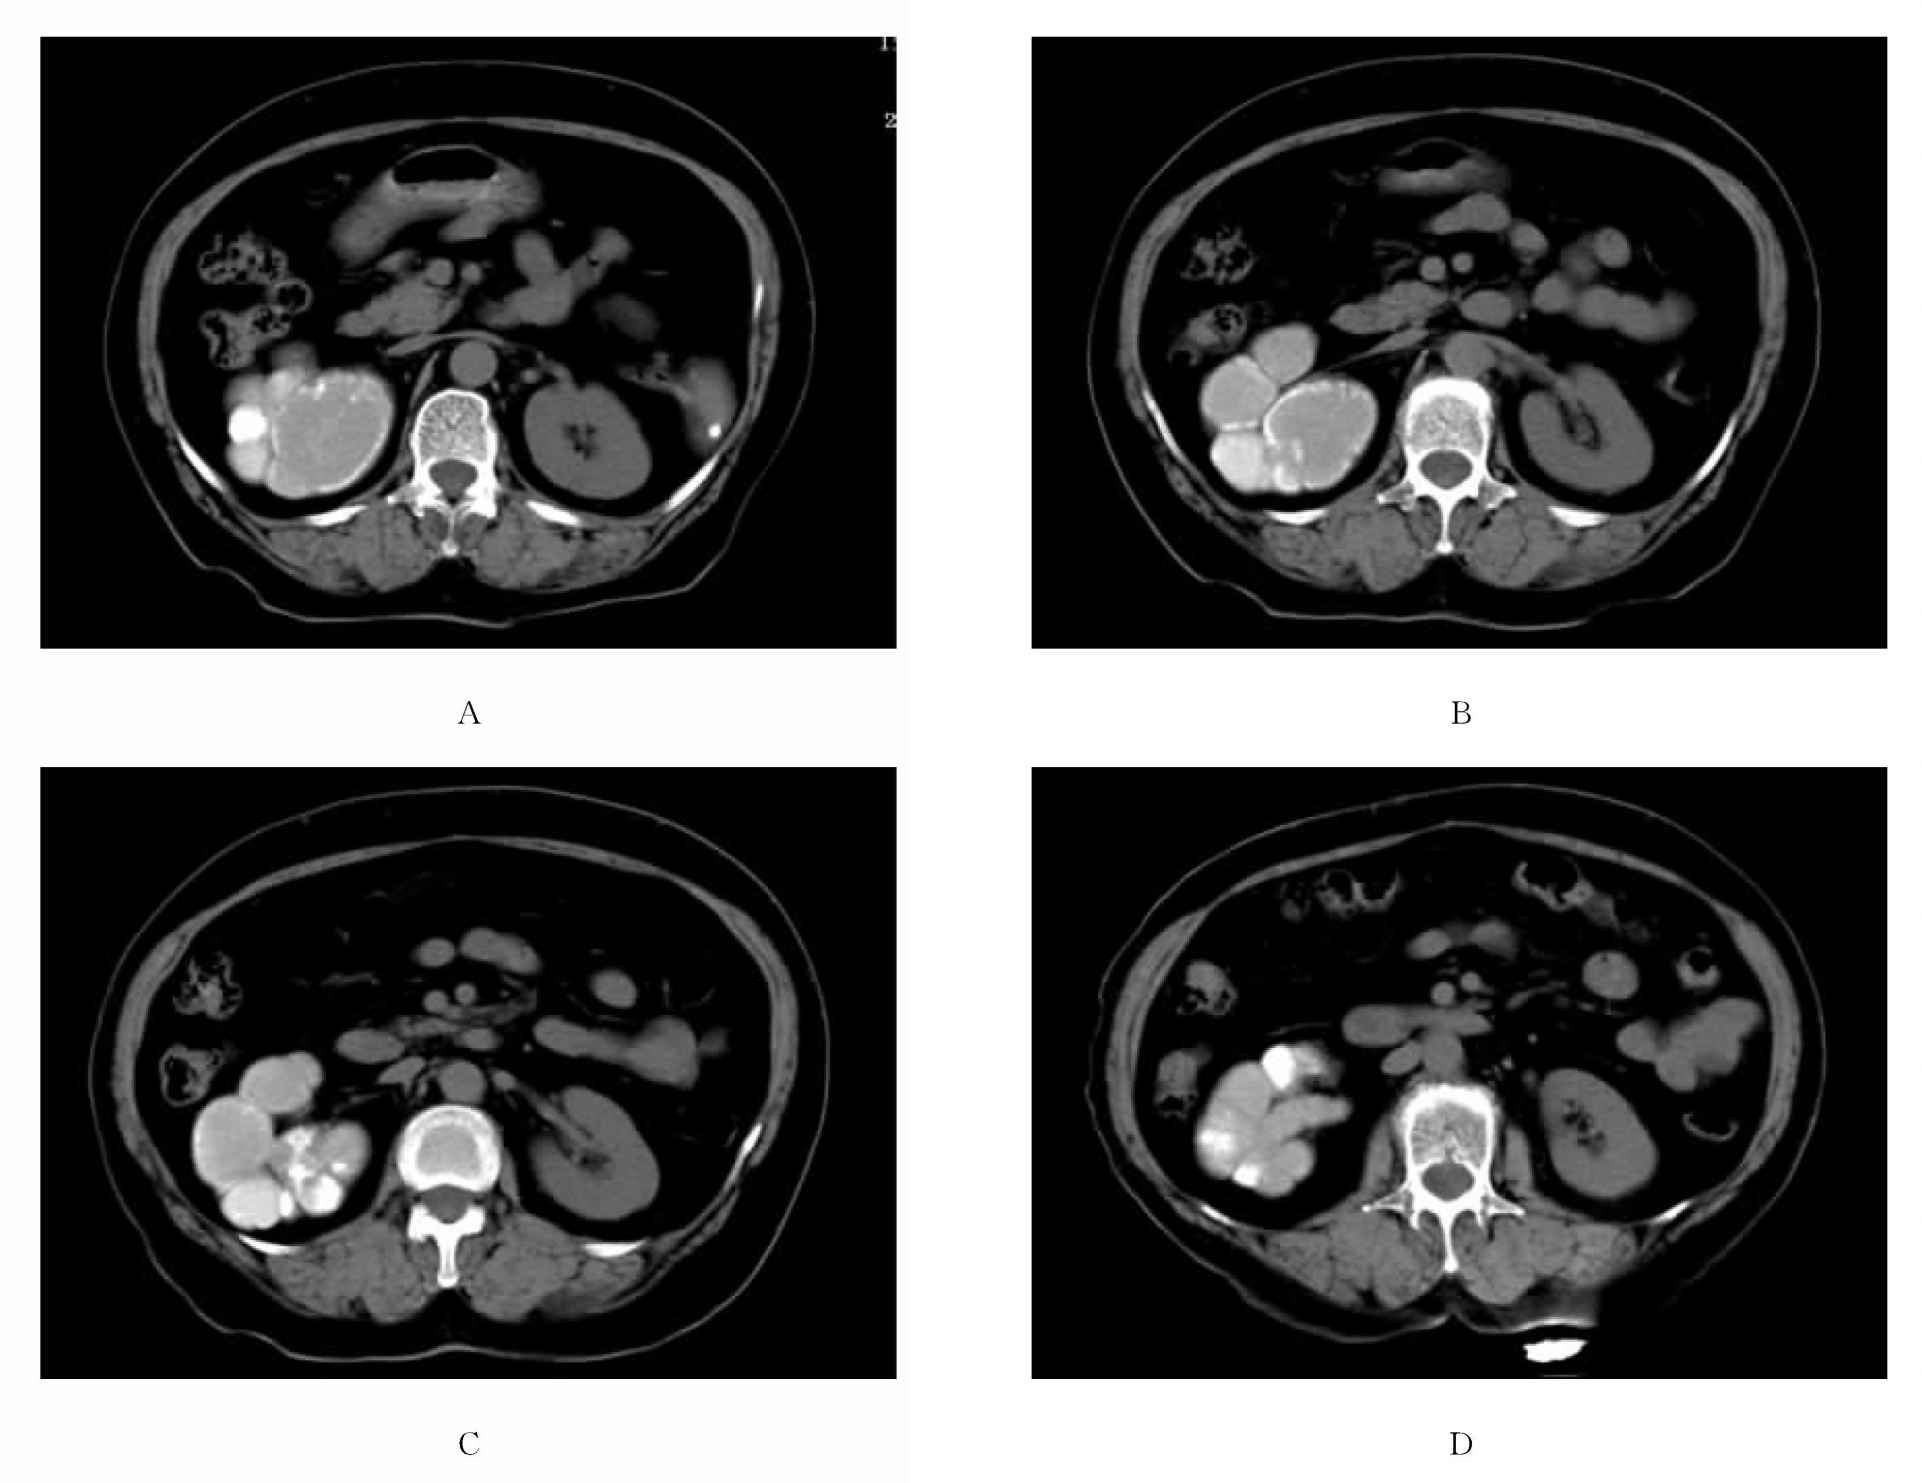
\includegraphics[width=.7\textwidth,height=\textheight,keepaspectratio]{./images/Image00327.jpg}
 \captionsetup{justification=centering}
 \caption{右肾结核\\{\small A~D为同一患者,右侧肾盏扩张为主,其内密度增高(钙质沉着),边缘和肾内有钙化,肾实质显著变薄;肾盂边缘毛糙}}
 \label{fig15-12}
  \end{figure} 

7.肾盂、肾盏及输尿管壁增厚:为较特征征象。

8.肾周侵犯:如肾周积脓或包膜下积脓。严重者可形成瘘道,如皮肤瘘道或肠瘘。

9.类似肿瘤样改变:个别可见。可能为结核球融合形成的较大结节,可见周边不规则钙化,并可向肾周侵犯。大小数厘米甚至达10cm。

以上表现并不一定同时出现。国外资料统计,最常见的CT表现为肾盏扩张(88%)、肾实质内斑痕(80%)和钙化(37%~71%),钙化和狭窄是其较为特征的表现。

\subsection{输尿管结核}

本病多由肾结核蔓延而来,也可由膀胱逆行感染所致。50%的泌尿系结核伴有输尿管结核。

\textbf{【病理】}
病变早期输尿管黏膜破坏,溃疡形成,管径扩大;后期因结核肉芽组织形成,管壁增厚、僵直,管腔狭窄甚至闭塞。输尿管壁可部分或全部钙化。

\textbf{【临床表现】} 其临床表现同肾结核。

\textbf{【CT表现】}
①输尿管管壁增厚:输尿管管壁的慢性增殖性改变,表现为输尿管周围的低密度影。②输尿管狭窄:晚期可导致管壁纤维化、瘢痕、狭窄变形,远端1/3部分最易受累(最常见于第三生理狭窄处)。狭窄以上输尿管扩张、积水。狭窄常呈多发性,并示扩张与狭窄交替存在。严重者可致输尿管闭锁。③输尿管管壁钙化:注意与结石鉴别。

\subsection{膀胱结核}

本病多继发于肾结核,也可由周围结核蔓延所致。

\textbf{【病理】}
早期膀胱黏膜充血、水肿,形成不规则溃疡和(或)肉芽肿,开始于患侧输尿管口处,其后蔓延至三角区乃至全部膀胱。晚期肌层广泛受侵,膀胱壁增厚并发生挛缩。

\textbf{【临床表现】}
主要表现为尿频、尿急、尿痛即膀胱刺激征,以及持续性脓尿和血尿,还可有低热、乏力、消瘦等。

\textbf{【CT表现】}
早期病变多位于输尿管口附近,可表现为膀胱壁局部结节或局部僵硬、增厚;中晚期表现为膀胱壁广泛增厚、膀胱容积缩小、轮廓毛糙,即所谓的“挛缩膀胱”(图\ref{fig15-13});少数可见膀胱壁钙化,呈不规则条索状或斑片状。增强扫描病变表面线状强化提示病变活动。

\begin{figure}[!htbp]
 \centering
 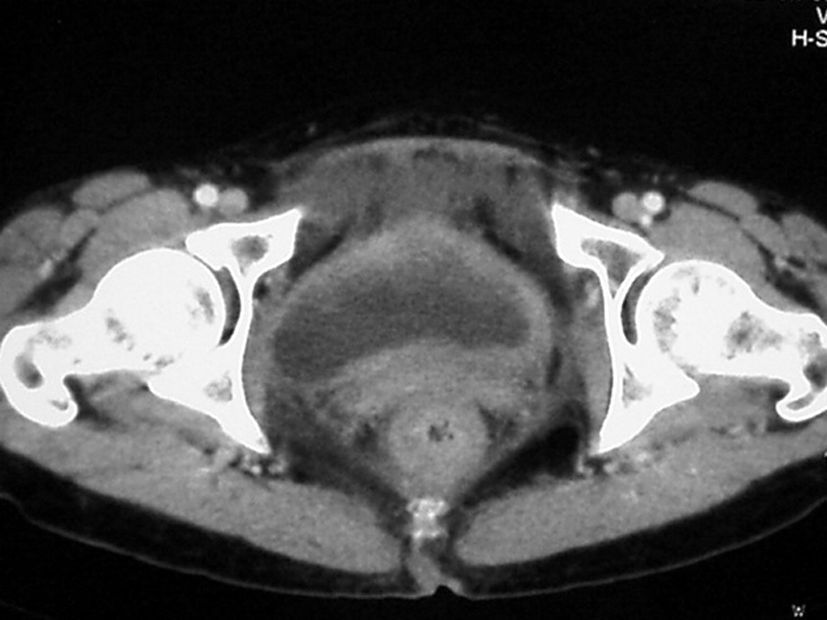
\includegraphics[width=.7\textwidth,height=\textheight,keepaspectratio]{./images/Image00328.jpg}
 \captionsetup{justification=centering}
 \caption{膀胱结核\\{\small 膀胱容积缩小、轮廓毛糙,精囊腺边缘也毛糙}}
 \label{fig15-13}
  \end{figure} 

\textbf{【鉴别诊断】}
有时可见由结核病灶引起的充盈缺损,类似膀胱癌。但膀胱癌容积不缩小,且结核多有肾及输尿管病变;此外,膀胱结核患者尿液密度偏高,常有絮状物;肿瘤患者膀胱内呈水样密度(出血者除外)也有助于鉴别。

\subsection{肾真菌感染}

此病较为少见,预后很差。

\textbf{【病因】}
泌尿系真菌感染以白色念珠菌最常见,其次为曲霉菌,其他少见。常发生于糖尿病和多种免疫功能低下的患者。肾念珠菌感染常由全身性念珠菌血症引起,但经膀胱的逆行感染同样是重要途径。

\textbf{【临床表现】}
呈急性感染的症状,预后很差;严重者可发生真菌性败血症,全身器官均可受累,常引起死亡。部分呈慢性过程,症状可不明显。

\textbf{【CT表现】}
①多类似于急性肾盂肾炎或多发小脓肿:肾随时间(数日到数周)逐渐增大;肾实质密度不均匀,内有多个斑片状低密度区,也可混杂高密度出血;真菌脓肿则呈壁较厚的类圆形低密度灶;常有肾周感染。增强扫描有不规则强化,真菌脓肿壁呈环形强化。②部分呈慢性过程,CT表现可类似慢性肾盂肾炎,如肾功能减退、瘢痕形成和肾盏变钝等。③真菌球:呈肾盂肾盏内充盈缺损表现,如在充盈缺损内发现花边状透亮的气体影,则具诊断意义。但真菌球常难以与凝血块及肿瘤鉴别。

\subsection{肾包虫病}

\textbf{【病因病理】}
本病是由于人吞食细粒棘球蚴的虫卵经消化道传染而致。70%发生于肝脏,20%发生于肺,仅约1%发生于肾脏。在肾内常单发,在母囊内有子囊,内囊为棘球蚴虫囊,外囊为宿主形成的纤维包膜,囊内含有液体。

\textbf{【临床表现】}
本病在临床上症状不明显,生长缓慢,常体积很大时才被发现或触及肿块,多数肾功能已遭到严重破坏,而出现相应的症状。

\textbf{【CT表现】}
肾体积增大,内含水样密度的囊肿。囊肿单发或多发,大小不一;呈圆形或椭圆形,边缘光滑整齐。囊壁厚薄不均,有强化。母囊内出现子囊,即囊内囊征有一定诊断价值。母囊的壁一般较子囊的壁密度高、厚度大,有时囊壁也可钙化。若同时合并肝包虫病则更易做出诊断。

\subsection{膀胱炎}

膀胱非特异性炎性病变主要靠病史、细菌培养、膀胱镜检查和活检证实,影像学对诊断的作用不大。

\textbf{【病因病理】}
本病多为继发性,其病因很多,可分为细菌性和非细菌性两类。大多为细菌性感染,病原体常为大肠杆菌,其次为葡萄球菌。非细菌性包括很多物理因素(如创伤、放射损伤等)和化学因素(如一些抗癌及其他的药物治疗)。

急性膀胱炎病理上见黏膜和黏膜下层的充血、水肿,甚至可有出血和溃疡。严重者可涉及肌层。慢性膀胱炎病理上见膀胱壁不规则增厚并有小梁形成,常有膀胱容积缩小。膀胱壁内含气见于气肿性膀胱炎或泌尿系器械检查后,或膀胱与肠道间有瘘道。

结盖性膀胱炎、气肿性膀胱炎、嗜酸性膀胱炎、腺性膀胱炎、囊性膀胱炎、间质性膀胱炎为膀胱的特殊炎症。结盖性膀胱炎就是在炎性病灶上有假膜覆盖,且由于细菌(可能为产碱杆菌)的作用使尿液内钙质(大多为磷酸盐)沉着其上。气肿性膀胱炎好发于糖尿病人,因产气细菌(大肠杆菌及其他产气杆菌、球菌等)的作用,使膀胱壁内有很多积气(可能来自发酵的葡萄糖)。嗜酸性膀胱炎为泌尿道过敏性疾病。腺性膀胱炎是一种引起膀胱黏膜高度增生的炎症。

\textbf{【临床表现】}
多数膀胱炎见于妇女,常合并尿道炎和阴道炎。急性膀胱炎患者有尿频、尿急、尿痛,往往较严重,并有脓尿和不同程度的血尿。慢性膀胱炎症状相对较轻,但如有膀胱容积缩小者,仍有尿频;尿液检查有白细胞增多和红细胞。膀胱炎病情严重或并发肾盂肾炎及其他急性感染时有全身症状。

\textbf{【CT表现】}
CT除见膀胱壁增厚外,无特征性表现(图\ref{fig15-14})。还可见膀胱边缘广泛不规则、毛糙,膀胱容积缩小。并发梗阻可有小梁形成,表现为波浪状或憩室样突出。

\begin{figure}[!htbp]
 \centering
 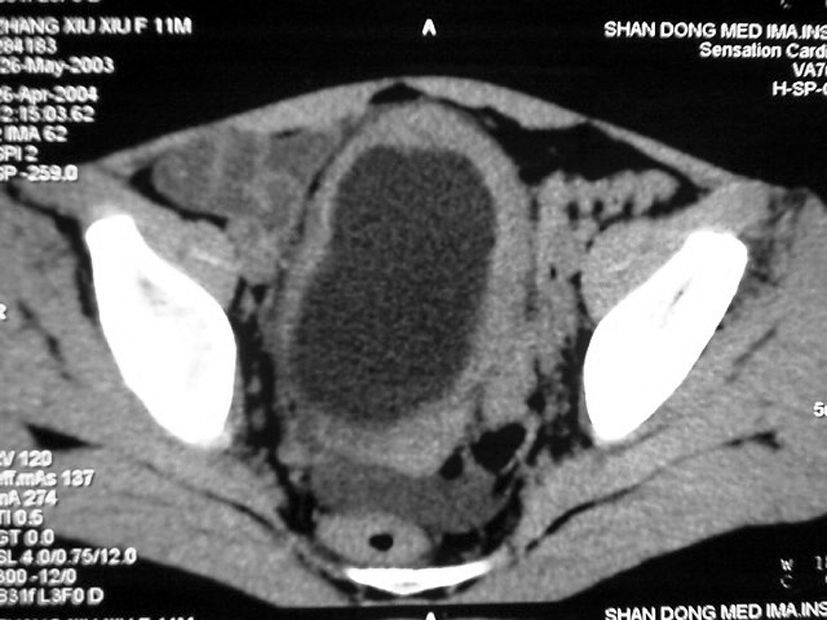
\includegraphics[width=.7\textwidth,height=\textheight,keepaspectratio]{./images/Image00329.jpg}
 \captionsetup{justification=centering}
 \caption{膀胱炎\\{\small 膀胱壁显著增厚,边缘较光滑}}
 \label{fig15-14}
  \end{figure} 

此外,①结盖性膀胱炎CT可见膀胱壁小斑片状钙化,但应与膀胱裂体吸虫病相鉴别,后者可引起广泛大片钙化。②气肿性膀胱炎CT表现膀胱壁内有低密度气带及气泡。③嗜酸性膀胱炎CT表现膀胱壁局限性或弥漫性不均匀增厚、僵硬,并可呈团块状向腔内突出,膀胱周围可有侵犯。与膀胱肿瘤易于混淆。④腺性膀胱炎CT表现膀胱占位合并膀胱壁较广泛增厚,而无壁外侵犯,应高度怀疑本病。

\subsection{嗜酸性膀胱炎}

本病为泌尿道过敏性疾病。

\textbf{【病理】}
膀胱黏膜及黏膜下充血、水肿,肌肉坏死及表层肌肉有纤维化等损害。显微镜下以膀胱黏膜大量嗜酸性白细胞浸润为特征。

\textbf{【临床表现】}
似一般膀胱炎,有尿频、尿急、尿痛,并可见血尿。化验检查血、尿液中嗜酸性白细胞增多,血尿、脓尿、蛋白尿。膀胱镜可见黏膜红肿和广基息肉状新生物,与肿瘤相似。抗感染、抗过敏治疗较短期即可治愈,预后佳。

\textbf{【CT表现】}
包括其他影像学表现不具特征,与膀胱癌难以鉴别。CT可表现为膀胱壁局限性或弥漫性不均匀增厚、僵硬,并见软组织团块突向腔内,膀胱周围脂肪间隙内可见条片状浸润性密度增高影。

所以,如发现宽基底肿物、临床表现似膀胱炎时,需注意结合临床排除嗜酸性膀胱炎。

\subsection{腺性膀胱炎}

本病是一种较罕见的慢性病变,常伴非特异性感染,又有发展成膀胱癌的可能。

\textbf{【病因】}
尚不明确,可分为两种:①胚胎残余的发展:直肠从尿生殖隔分离时,可能有异位胚胎残余遗留,在一定情况下转化成腺成分。化生过程则由炎症所致,若进一步发展可致腺性膀胱炎,也可再发展成恶性病变。②移行上皮化生:当膀胱受到长期的感染、结石、梗阻或者其他一些中毒因素的慢性刺激后,黏膜上皮先形成上皮芽,伴有上皮芽的移行上皮细胞向下增殖,可分化成为真正的腺体,成为腺性膀胱炎或者发展为腺癌。

\textbf{【病理】}
腺性膀胱炎的特征是含有黏液的柱状上皮细胞位于黏膜表面或形成腺体向下长入固有层内,故CT增强效应不明显。还有人认为它与囊肿性膀胱炎是同一疾病的不同过程,因向下增殖的上皮细胞首先可形成囊肿,即囊肿性膀胱炎,继之可形成真正的腺体及腺性膀胱炎。本病与膀胱肿瘤的关系可能有3种:①黏膜增生改变先于肿瘤;②肿瘤发生于黏膜增生性改变之间;③两者同时发生。

\textbf{【临床表现】}
尿频、尿急、尿痛,排尿困难或肉眼血尿。少数患者可引起双侧输尿管梗阻而导致肾积水,腰部酸胀等症状。病理检查是本病确诊的依据。

\textbf{【CT表现】}
病灶好发于膀胱后壁,常呈隆起性病变或膀胱壁增厚;病变范围可比较局限,也可以累及整个膀胱壁;病变表面较光滑且延续。部分病例可有囊肿及蛋壳样钙化形成。增强扫描病灶强化不明显且与周围正常膀胱壁相似。可累及输尿管末端引起肾积水。膀胱外缘光滑即无外侵,且盆腔淋巴结无增大。

总之,当发现膀胱占位,合并膀胱壁较广泛增厚且无壁外侵犯时,应高度怀疑本病。

\textbf{【鉴别诊断】}
可从下列几方面与膀胱肿瘤相鉴别。①病灶的形态及内部结构:腺性膀胱炎一般病灶表面较光滑,可有囊肿及蛋壳样钙化;膀胱肿瘤因缺血坏死表面不光整,肿块和龛影同时出现,可有液性坏死区及斑点状钙化。②盆腔淋巴结及膀胱外膜层:腺性膀胱炎的膀胱外膜层光滑,且无盆腔淋巴结增大;晚期膀胱癌可有盆腔淋巴结增大及膀胱外层受侵而模糊。③增强扫描:腺性膀胱炎因病灶区是腺体组织,其强化不明显;而膀胱肿瘤由于血供丰富,增强扫描常有较明显的强化而高于膀胱壁。④诊断性治疗:腺性膀胱炎抗炎治疗有效;而膀胱肿瘤无效。

\section{肾脏囊性病变}

\subsection{概述}

肾脏的囊性疾病有多种类型,其分类见表\ref{tab15-1}。

\begin{table}[htbp]
\centering
\caption{肾脏囊性疾病及分类}
\label{tab15-1}
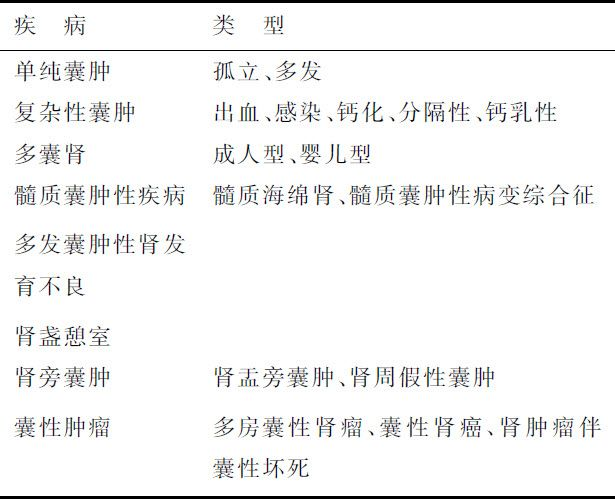
\includegraphics[width=\textwidth,height=\textheight,keepaspectratio]{./images/Image00330.jpg}
\end{table}

\subsection{单纯性肾囊肿}

\textbf{【病因病理】}
囊肿起源于肾小管。本病与遗传因素无关。可为先天性或后天因素所致。目前多认为是肾小管阻塞或部分肾组织缺血所致。其发生率与年龄有关,多见于50岁以上,30岁以前罕见,提示与肾脏的退行性变有关。尿毒症透析患者其发生率明显增加(属获得性肾囊肿)。肾囊肿中2.1%~3.5%同时有肾癌。单纯囊肿并发囊壁癌不足1%。病理上囊肿可单发或多发。大小可自数毫米至十几厘米。囊肿多发生在肾实质中,尤以皮质多见。囊壁由一薄层纤维组织覆盖以一层扁平上皮,囊内含透明的浆液性液体,少数含血性液体。囊内偶有分隔,囊壁偶可钙化。

特殊类型肾囊肿又称为复杂性肾囊肿。主要包括以下几类:①高密度肾囊肿;②出血性肾囊肿;③感染性肾囊肿;④钙化性肾囊肿;⑤钙乳性肾囊肿;⑥分隔囊肿。

\textbf{【临床表现】}
大多无症状,囊肿大者患侧偶有轻度不适、高血压、蛋白尿等。囊肿破裂可出现腰痛及血尿,肾功能正常。

\textbf{【CT表现】}
平扫呈圆形或椭圆形低密度灶。大多位于皮质内,多为孤立单发,但双侧和(或)多发也不少见(图\ref{fig15-15})。囊肿内部密度均匀,CT值在-5~15Hu之间。但<10mm的小囊肿,因部分容积效应而密度升高。增强扫描囊肿无强化。囊肿与肾实质分界锐利、清楚。囊壁菲薄,不能显示,以致向肾外缘突出的囊肿,囊肿与肾外缘交界处呈鸟嘴征象。囊肿局限于肾筋膜内;肾盂肾盏可变形,但无截断破坏表现。

\begin{figure}[!htbp]
 \centering
 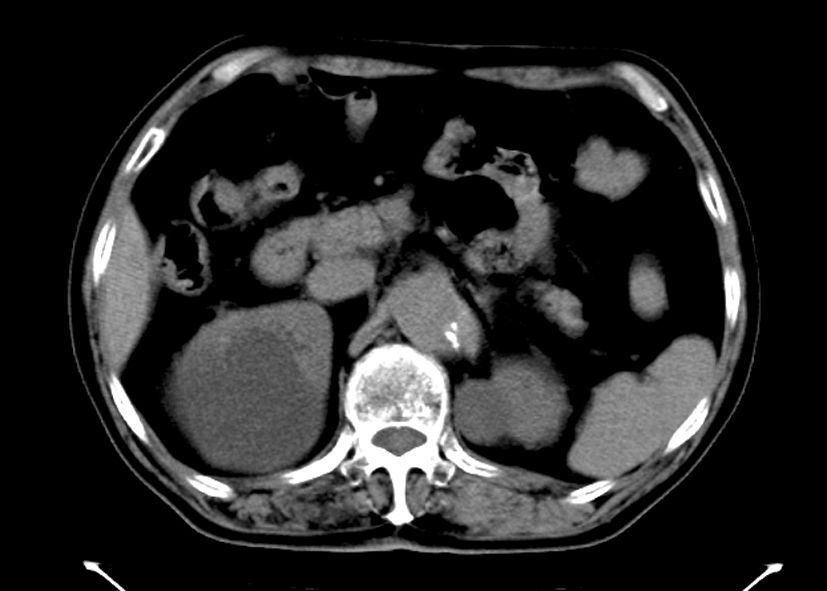
\includegraphics[width=.7\textwidth,height=\textheight,keepaspectratio]{./images/Image00331.jpg}
 \captionsetup{justification=centering}
 \caption{肾囊肿\\{\small 左右肾均有水样密度灶,边缘锐利、光滑}}
 \label{fig15-15}
  \end{figure} 

特殊类型肾囊肿表现如下:

1.高密度肾囊肿:其病因有囊肿内出血、高蛋白摄入、囊肿穿刺、钙乳性肾囊肿等,但高蛋白囊肿罕见。CT平扫为高密度,无强化。

2.出血性肾囊肿:出血原因有创伤、囊壁静脉曲张或出血性素质等。CT表现急性期为高密度,亚急性、慢性出血为等密度或低密度,均无强化。但囊壁可因纤维增生而增厚,且囊壁可有钙化。

3.感染性肾囊肿:可为血源性或手术穿刺等医源性感染。CT表现囊壁明显增厚、囊肿密度增高,增强扫描囊壁可无或有轻度强化。偶而可见囊内气泡及囊壁钙化。

4.钙化性肾囊肿:出血和感染是钙化的两大原因。最常见为周边环状钙化,其次是中央与周边钙化并存,单纯中央钙化最少见。

5.钙乳性肾囊肿:原因不明,可能与慢性炎症刺激有关。CT呈圆形或椭圆形高密度灶,大小0.3~3cm不等,多<1cm。轮廓光滑,密度均匀或不均匀,CT值多>100Hu,但低于结石。如见到钙液面可予确诊。

6.分隔囊肿:又称分房囊肿。其间隔薄而光滑,一般<1mm,连接于囊壁上,无增强。有时可见沿分隔分布的细条状钙化。

\subsection{肾盂源囊肿}

有学者认为不应归为肾囊肿的范畴,而称为肾盏憩室更确切。但也有学者认为两者病理基础不同。本病多为先天性。

\textbf{【病理】}
肾盂源囊肿大小约为2~4cm。大多位于肾髓质部,且在大肾盏或肾盂旁,与囊肿之间常有一细管相通,但在发生炎症时此管可闭塞。由于引流不畅,故常发生感染并有结石形成。

\textbf{【临床表现】}
一般无症状。可有患侧肾区疼痛,并有间断性脓尿。如囊肿不与肾盂肾盏相通而发生感染时甚似急性肾脓肿。

\textbf{【CT表现】}
囊肿位于肾实质内,其内可有结石。增强扫描因与收集系统相通,故造影剂充盈呈高密度,但难以发现与肾盂肾盏相通的细小管。合并感染可见囊壁增厚,增强扫描囊壁可无或有强化。

\textbf{【鉴别诊断】}
应注意与肾盂旁囊肿鉴别。两者均可能为先天性疾病,结构与单纯肾囊肿相似。两者均可有泌尿系感染症状。肾盂源囊肿与肾盂旁囊肿区别如下:①前者多位于髓质的肾柱区、大肾盏或肾盂旁;后者起源于肾实质外之肾窦,可能为慢性炎症所致的淋巴性扩张。②前者多与肾盂肾盏有细小管相通;而后者则无。③肾盂源囊肿由于引流不畅,常可发生感染并有结石形成;肾盂旁囊肿主要对输尿管及肾盂产生压迫。④前者CT表现囊肿位于肾实质内;后者位于肾门处与肾实质分开,囊肿周围有更低密度脂肪晕圈是其特征性表现(也是与单纯囊肿的鉴别关键)。⑤增强扫描肾盂源囊肿因与收集系统相通,故造影剂充盈呈高密度;而肾盂旁囊肿无强化。

\subsection{肾盏憩室}

有人认为肾盏憩室是肾盂源囊肿,但其病理基础不同,既不是先天性的。

\textbf{【病因病理】}
肾盏憩室是由于肾盏颈部的肌肉功能紊乱,局部肌肉发生痉挛收缩,以后因缺血而纤维化,进而发生狭窄阻塞。在其远端部分的肾盏就可以扩大呈囊状而成为憩室。狭窄处为肾盏与憩室的通道。憩室多较小,大者可达2~3cm,若无相通的管道存在,就可称为异位肾盏。

\textbf{【临床表现】}
与肾盂源囊肿相似,一般无症状。可有患侧肾区疼痛和间断性脓尿。

\textbf{【影像学表现】}
因憩室有分泌功能,故IVP和CT增强扫描可见造影剂充盈的憩室影。呈圆形或椭圆形,边缘光滑。少数可见憩室与肾盏之间的长2~3mm,宽约2mm的通道。较大的憩室因尿液潴留而稀释了造影剂,因此密度可相对较低。动态观察憩室内造影剂浓度逐渐增高,而肾盂肾盏内的造影剂逐渐排空,诊断可以肯定。

\textbf{【鉴别诊断】}
肾盂源囊肿延迟动态观察密度往往不能增高,而且常在局部的肾盏边缘造成压迹,可予鉴别。

\subsection{肾盂旁囊肿}

本病起源于肾实质外的肾窦,不与收集系统相通。

\textbf{【病因病理】}
病因尚不明,可能系先天性,也可能为慢性炎症所致的淋巴管囊性扩张。囊肿可为单发或多发、单房或多房,大小差异很大。其结构与一般囊肿相似,其壁有纤维组织。

\textbf{【临床表现】}
主要由肾盂、输尿管受压迫而引起,有肾区疼痛、血尿及感染的症状。

\textbf{【CT表现】}
囊肿位于肾门处与肾实质分开(图\ref{fig15-16}),囊肿周围有更低密度脂肪晕圈是其特征性表现,也是与单纯囊肿的鉴别关键。增强扫描囊肿无强化,有助于与肾盂积水相鉴别;同时增强扫描可见显影的肾盂、肾盏和输尿管受压、拉长,将囊肿衬托得更清晰。

\begin{figure}[!htbp]
 \centering
 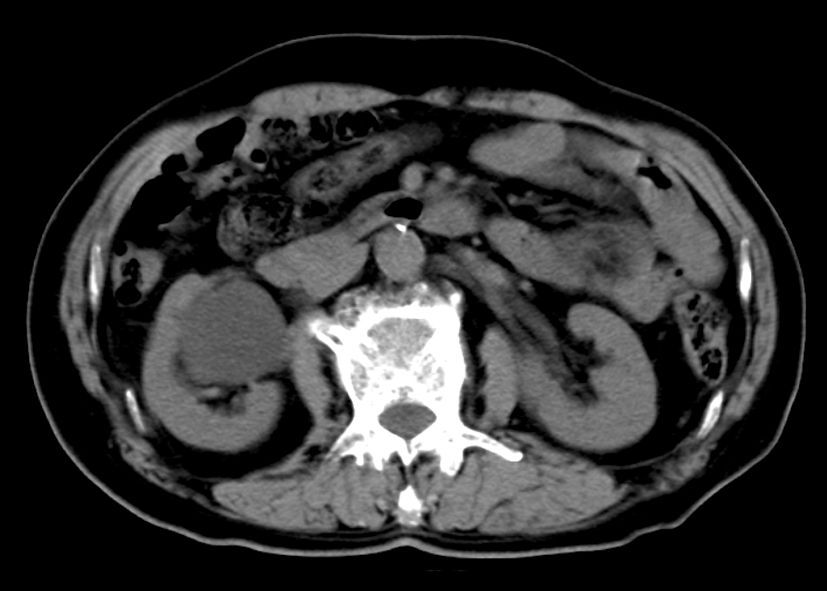
\includegraphics[width=.7\textwidth,height=\textheight,keepaspectratio]{./images/Image00332.jpg}
 \captionsetup{justification=centering}
 \caption{肾盂旁囊肿\\{\small 右侧肾窦区有水样密度灶,边缘锐利,周围有肾窦的脂肪环绕}}
 \label{fig15-16}
  \end{figure} 

\subsection{多囊肾}

\textbf{【病理】}
本病为肾皮质和肾髓质出现无数囊肿的一类遗传性疾病,按遗传方式分为两类。

1.婴儿型:是常染色体隐性遗传性疾病。以肾收集小管扩张和肝内胆管扩张及纤维化为特征,临床表现取决于病期及肾、肝受累程度。该型又分为3个亚型。①婴儿型:是该型中最常见的一类。多见于6个月以下的婴儿。60%以上肾实质受累,肝病变轻微。双肾明显增大,表面光滑。切面呈海绵状,为无数扩大、延长的收集管和肾小管长梭形或柱状扩张,自肾门向表面放射状排列;肾盂、肾盏受压。肝内小胆管增生、扩张、延长,常有门脉周围纤维化。②中间型:多见于6月至3岁的婴幼儿。其肾、肝病变各半或肾囊性病变较突出。③儿童型:多见于3~6岁或年长儿童。以肝受累为主。肝脏之胆小管为慢性囊性发育不良及显著门脉周围纤维化,部分病例并发胆总管或其他肝外胆管异常。肾小管扩张较轻且局限。

2.成人型:为常染色体显性遗传性疾病。虽多见于成人,亦可见小儿,尤其有家族史者。囊肿起源于近端肾曲管、肾小囊及肾小管,多为双侧受累而以一侧较突出。肾脏大小可正常,或随囊肿的发展而增大,表面不光滑。切面肾实质内有多数大小不等、薄壁、含浆液的球形囊肿,囊肿间的肾实质受压及萎缩影响肾功能。囊性病变也常见于肝,偶有肝胆管增生与肝纤维化。少数胰、脾、肺、卵巢、甲状腺、睾丸、精囊内也存在囊肿,也可并发脑Willis血管环小动脉瘤(15%)。

\textbf{【临床表现】}

1.婴儿型:①婴儿型:多于出生后不久死于尿毒症或呼吸窘迫。存活者都有持续性高血压,最后发展成终末期肾衰。②中间型:临床可伴高血压、肾功能低下、肾性骨营养不良,少数肝大或早期门脉高压症状较突出。③儿童型:主要表现为肝、脾肿大及门脉高压。

2.成人型:多在40~60岁出现症状。临床可无症状或表现为腰痛、恶心、呕吐、血尿、尿路感染症状,以及高血压和局部肿块,最后出现肾功能不全表现。

\textbf{【CT表现】}

\subsubsection{婴儿型}

1.婴儿型:双肾明显增大,密度普遍不均匀减低,CT值较正常肾偏低(30~35Hu),肾叶间隔较密,构成轮辐状。增强扫描示肾实质显影迟缓,皮髓质分界不清,肾密度不均匀呈细网状,或见条形肾图,以髓质部分明显,肾盂肾盏显影延迟至数小时到24小时。

2.中间型:肾影增大,实质内密度低,见小囊状低密度区。增强后肾实质密度不均,可显示高密度的小囊状充盈及条状影,主要位于髓质内。肾盂肾盏可分辨,并有变形。

3.儿童型:双肾正常或轻度增大。增强扫描肾功能正常或稍低,肾髓质密度增高并可呈斑条状,肾皮髓质分界清楚。此外,肝内胆管轻度扩张,有肝硬化及门脉高压等征象。

\subsubsection{成人型}

与婴儿型的CT表现有别。表现为肾影正常或增大,轮廓较光滑或分叶。肾实质内有许多分散的囊状水样低密度灶,界限清楚,大小不等(图\ref{fig15-17});增强扫描无强化。肾盂(盏)可有或无变形拉长,因囊肿数目、大小、部位而异。

\begin{figure}[!htbp]
 \centering
 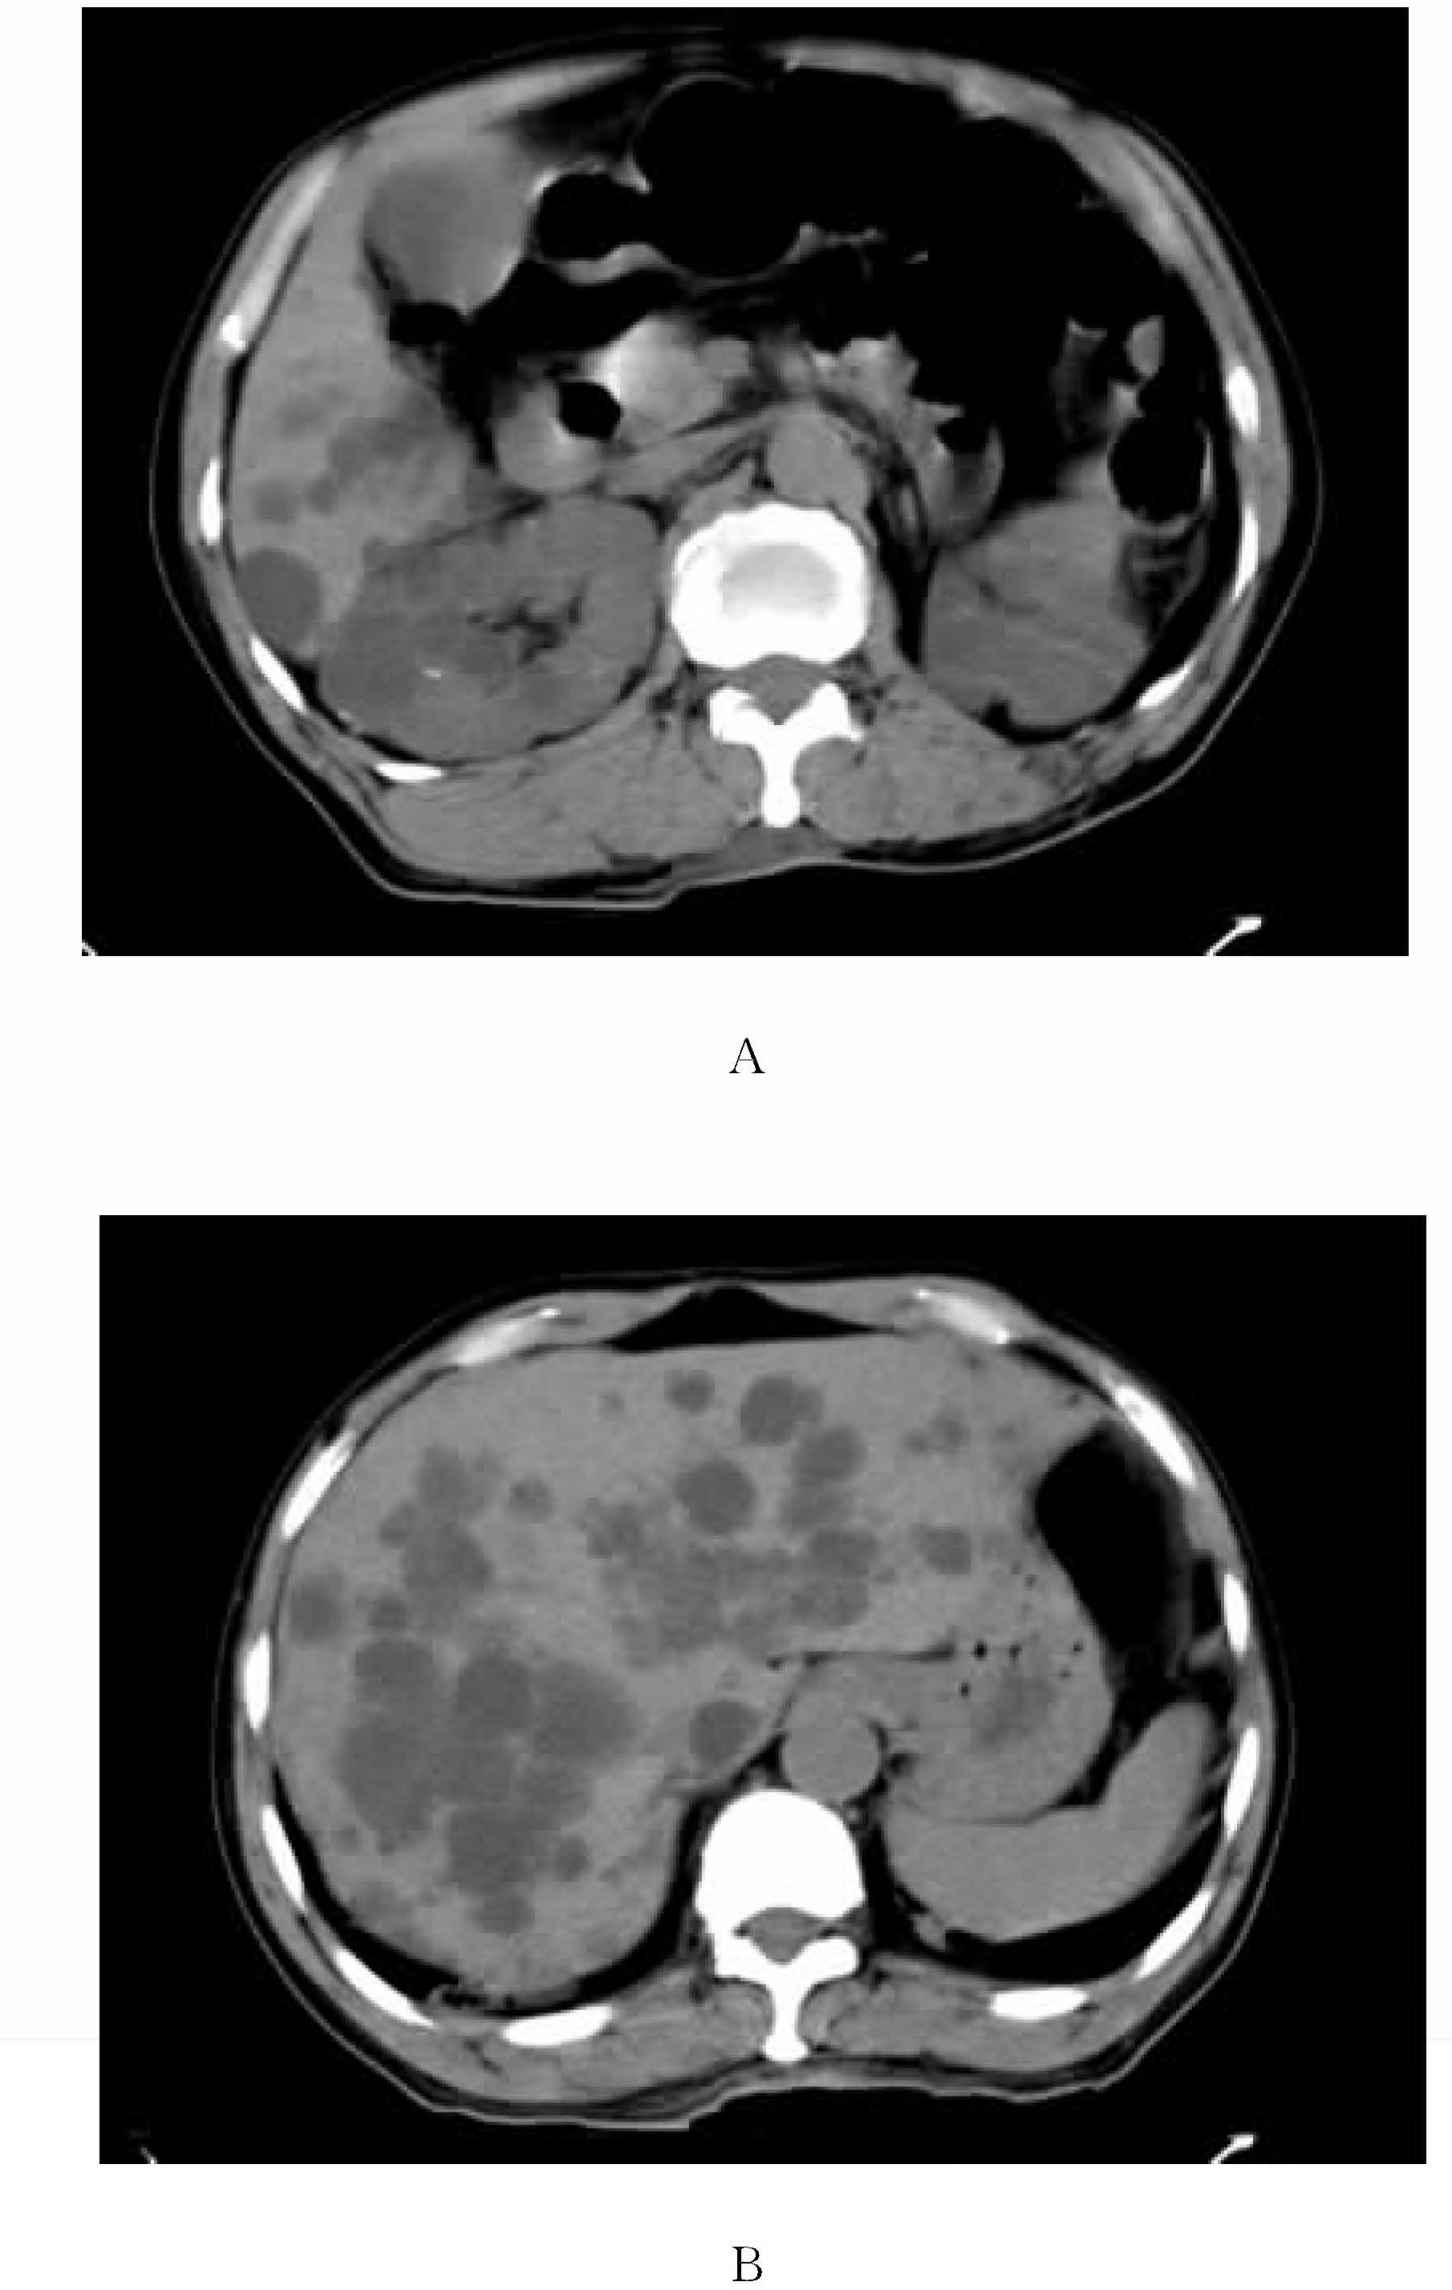
\includegraphics[width=.7\textwidth,height=\textheight,keepaspectratio]{./images/Image00333.jpg}
 \captionsetup{justification=centering}
 \caption{多囊肾\\{\small A、B为同一患者,A示双侧肾内有无数水样密度灶,B示合并多囊肝}}
 \label{fig15-17}
  \end{figure} 

成人型的并发症有:①囊肿出血:不常见。②继发感染:可表现为囊肿感染、气肿性肾盂肾炎、肾周脓肿。③阻塞:阻塞原因是大囊肿、钙化或血块压破和(或)阻塞肾盂漏斗部或输尿管。

\textbf{【鉴别诊断】}
多发性肾囊肿为非遗传性疾病,与多囊肾非同一疾病。两者区别如下:①多发性肾囊肿多发散在、囊肿间肾实质正常,病灶占肾实质的2/3以下,肾功能正常,无肝、脾、胰多发囊肿。②多囊肾的囊肿多发、密集、大小不一,囊与囊之间不相通,但囊与囊之间的实质受压萎缩。病灶多占肾实质的2/3以上,肾功能减退。多伴肝、脾、胰囊性病变。故“多囊肾”与“多发性肾囊肿”含义不同,但有时影像学鉴别困难。

\subsection{多发囊肿性肾发育不良}

本病又称为多囊性肾、多发囊肿肾,是一种非遗传性病变,为新生腹部肿块的常见原因之一。

\textbf{【病理】}
由一组大小不等的、互不相通的薄壁囊肿组成,囊肿间的肾组织发育不良,多无功能,所以是一种更严重的发育畸形。本病常累及单侧全肾,罕见节段局灶或双侧病变,常有对侧泌尿系先天异常。收集系统常有不同程度的闭锁和狭窄。肾动脉细或缺失,肾静脉细而扭曲。故与多囊肾是不同的。

\textbf{【临床表现】}
好发于新生儿和婴儿,多以腹部包块就诊。可有对侧泌尿系先天异常如肾盂输尿管交界处狭窄、肾旋转不良等。两侧多发囊肿性肾发育不良者常早期夭折。

\textbf{【CT表现】}
①小儿患者典型的表现为正常肾组织被异常肿块所替代,肿块由无数大小不等、水样密度的肿块组成,其间可见分隔并可增强。②成人患者还可表现为囊壁钙化、肾无功能,对侧肾代偿性增大。囊肿钙化常多发,但偶尔只见一个或一个为主的囊肿钙化。因成人腹膜后脂肪丰富,易显示肾血管蒂的异常。

\subsection{多房囊性肾瘤}

曾有多房性肾囊肿、囊腺瘤、囊性淋巴管瘤、囊性错构瘤、多房囊腺瘤等命名。现认为以多房囊性肾瘤命名最为合适,且该病应属良性肿瘤。本病是一种非遗传性罕见囊性病变。

\textbf{【病因病理】}
多数学者认为本病是先天性集合小管发育不全,肾小管囊性扩张所致;也有学者认为该病介于先天性畸形和肿瘤之间,其发展和肾母细胞瘤有关;还有报道部分病例有恶性倾向。病理显示由多个大小不等、互不交通的囊腔形成。外有厚壁、内有分隔(即含有一定的实性成分)。囊壁被覆单层立方和(或)扁平上皮。囊内有淡黄或棕色的浆液。间隔组织成分不尽统一,有学者认为是纤维化和分化良好的肾小管,不包括分化不良的组织和母细胞,如存在应诊断为部分分化性的肾母细胞瘤;还有学者认为可含纤维组织和胚细胞,甚至可与肾母细胞瘤混淆。

\textbf{【临床表现】}
好发于4岁以前男孩和40岁以上女性。临床症状无特殊性,通常无症状或主要为腹部肿块、腰痛,少数有高血压,偶有血尿。

\textbf{【CT表现】}
①多房性占位:通常>3cm。位于肾内或部分突向肾外,可有肾盂受压并积水。囊肿位于肾的一侧,且局限分布,有别于多囊肾;且各个囊之间无交通有别于淋巴管瘤。囊腔大小从几毫米至几厘米不等,但如囊腔<1cm,CT和B超亦难以鉴别。②边界清楚:囊壁可有弧形钙化,钙化位于边缘;而钙化形态多样,钙化外带有软组织成分多提示恶性。③囊内容物均匀或不均匀。④囊间隔均匀或厚薄不一:一般无明显结节影,囊间隔密度比正常肾实质低,分隔完全;增强扫描囊间隔有轻、中度延迟强化。国内有学者认为如果肿物厚薄较均一,呈轻、中度强化,则肿物的囊间隔以纤维成分为主;若间隔厚薄不一,实性成分较多,有结节状强化,那么囊间隔含有肾母细胞瘤病灶的可能性较大。但我们认为后者与囊性肾癌的鉴别可能是困难的。

总之,本病的影像学特征是单侧性、孤立性、多房性囊肿,边界清晰,各小囊间互不相通,小囊间隔薄(<1mm)而光滑、强化程度不如正常的肾组织。与肾局限性多发囊肿较难鉴别,后者少见,由多个单纯囊肿紧邻而成,可能的鉴别点是后者的边缘分叶较多房囊性肾瘤显著。

\subsection{髓质海绵肾}

本病的特征是一个肾或两个肾的锥体的集合管呈梭形或囊状扩张,致肾脏似海绵状,故称海绵肾。发病率为1/5000。

\textbf{【病因病理】}
多数学者认为是一种先天发育异常,可能由于肾源性胚基与输尿管胚芽异常连接所致。病变可局限于一个至多个肾锥体,以双侧多见。病理可见肾脏大小正常或因囊肿而稍增大,边缘光滑。剖面见锥体呈多孔状或海绵状,小囊腔多数为1~6mm,囊壁被覆立方和(或)扁平上皮。50%~90%囊内含有多发性小结石。晚期这些小囊可增大,继发感染可出现相应病理表现。

\textbf{【临床表现】}
多见于中年男性。轻者一般无症状,重者有血尿、脓尿、蛋白尿及反复发作的肾盂肾炎,甚至肾小管中毒症状。并发症晚期可出现肾功能尤其肾小管功能的损害。

\textbf{【CT表现】}
平扫可见肾锥体内多发斑点状小结石,呈散在、簇集成团或花环状等;或见肾锥内条纹状、小囊状低密度。增强扫描示注入造影剂数分钟后,造影剂充填肾锥体内扩张的集合管,使肾锥体呈现条纹状、刷子状、囊状或扇形高密度区,结石位于扩张的集合管内,扩张的集合管内造影剂排空较为延迟(图\ref{fig15-18})。

\begin{figure}[!htbp]
 \centering
 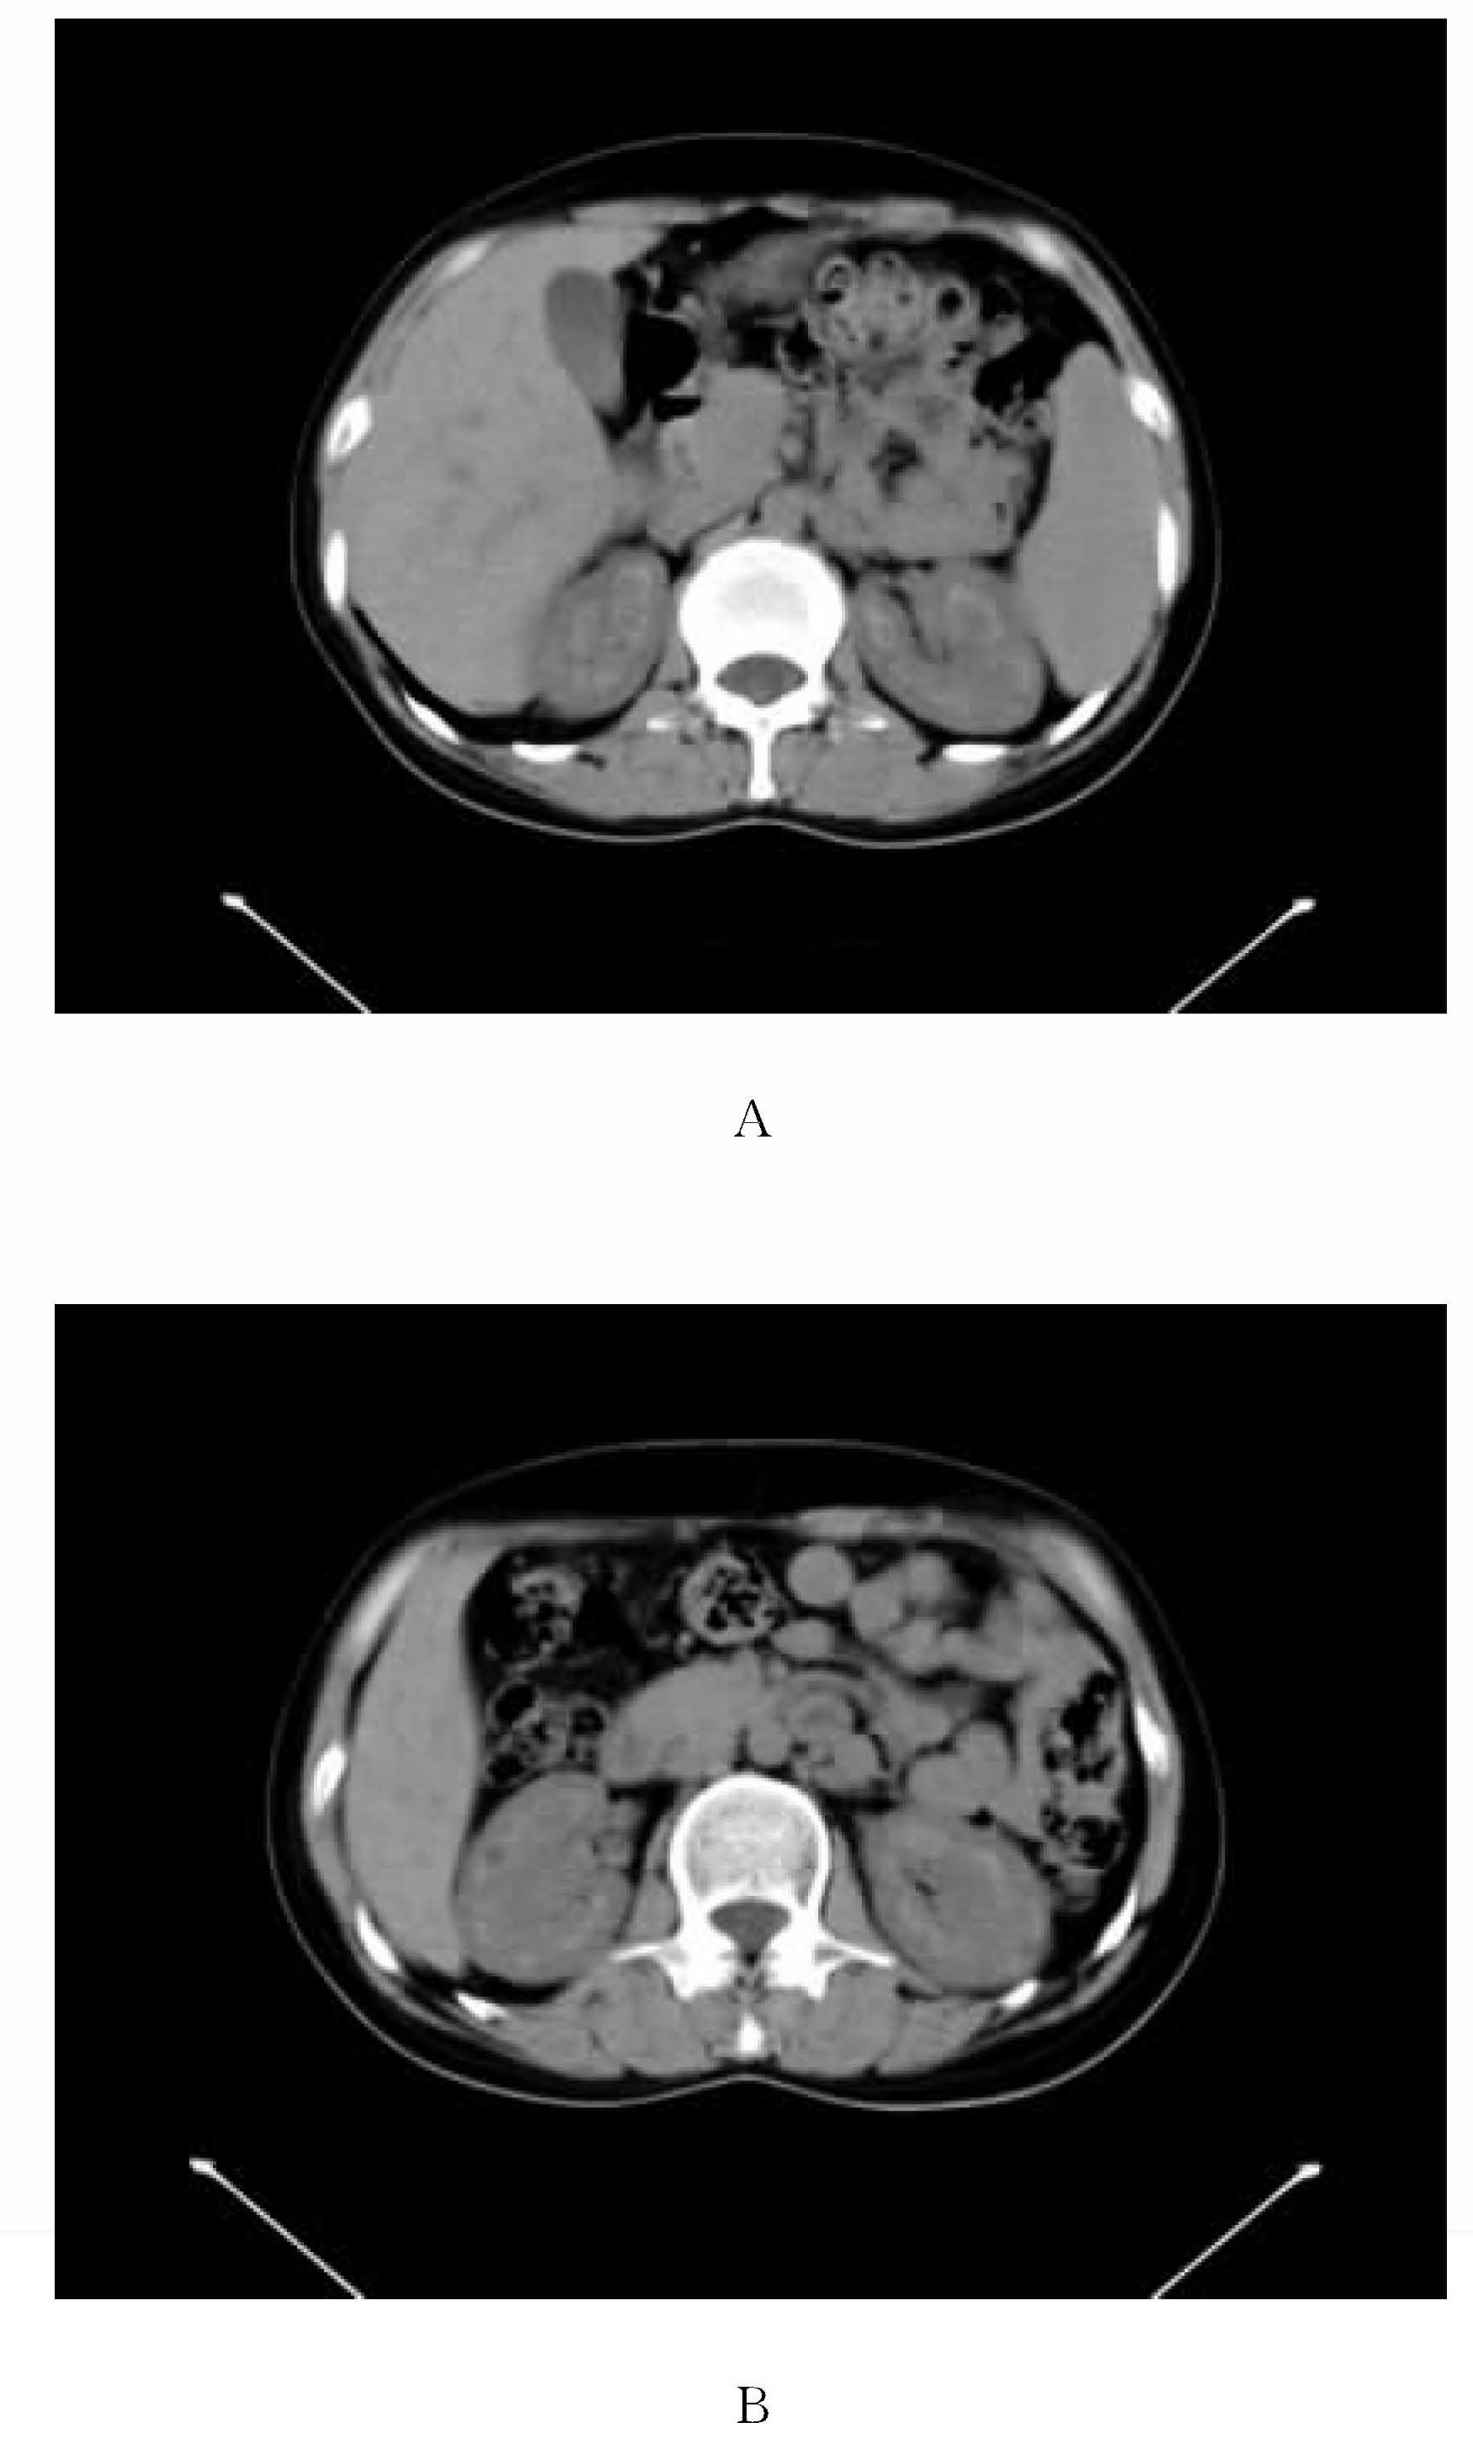
\includegraphics[width=.7\textwidth,height=\textheight,keepaspectratio]{./images/Image00334.jpg}
 \captionsetup{justification=centering}
 \caption{髓质海绵肾\\{\small A、B同一患者,肾锥体内多发班点状小结石,呈簇集成团、花环状}}
 \label{fig15-18}
  \end{figure} 

\textbf{【鉴别诊断】}
①肾钙质沉着症:见于甲状旁腺功能亢进、肾小管酸中毒、维生素D过多症、慢性肾小球肾炎等,一般无集合管扩张和乳头囊腔形成、钙化较弥漫且涉及肾皮质。②肾小盏内散发性小结石:位于肾盏内,可并发肾盂、肾盏轻度积水,位置可变动。③锥体潮红:是应用高浓度造影剂使锥体内肾小管显影,表现为乳头造影剂充盈呈轮廓不清之扇形影,造影剂排空与肾盏同步。

\subsection{肾髓质囊性病}

本病又称家族性青年性肾脏囊性病、范克尼(Fanconi)肾脏囊性病。本病为常染色体隐性遗传。

\textbf{【病理】}
它的特征是肾髓质有多发囊肿,直径自1mm~1cm;囊壁被覆扁平上皮。其余肾组织可见肾小球数目减少,肾小管萎缩,肾间质有弥漫性纤维化。

\textbf{【临床表现】}
症状开始于儿童或青壮年。①发育成长缓慢;②多尿、烦渴;③盐类消耗大,进行性尿毒症;④低血钙性抽搐;⑤高血压;⑥尿比重低且固定;⑦贫血。

\textbf{【CT表现】}
双肾对称性累及。肾皮质变薄;肾髓质呈低密度,较大的囊肿呈圆形或椭圆形低密度灶。增强扫描示肾显影迟缓,密度较低,尤以髓质部分更明显,其中可见数个稍大的不增强囊肿;皮质极薄,类似肾积水,但低密度区的密度高于水。

总之,除上述CT表现外,结合尿浓缩功能不良、静脉及逆行肾盂造影无明显异常,可提示诊断。

\subsection{肾周囊肿}

肾周囊肿是后天性的,大多由外伤所引起,通常是在肾周包裹性的尿样浆液的存在,故亦称为肾周积水。

\subsubsection{肾周渗尿}

由于肾盂肾盏外伤引起尿液漏到脂肪囊中,亦可由于肾盂积水破裂所造成。临床主要表现肾区胀痛,并可有感染及血尿。CT可明确显示肾周积液的存在。

\subsubsection{肾周血肿}

可由动脉瘤破裂、癌肿、错构瘤、结核破坏血管或其他出血性疾病引起血液在肾脂肪囊中呈层状积聚,以后边缘部分机化形成纤维包壳,其中央部分被透明液所替代。临床表现为肾区胀痛,且时有血尿。CT可明确诊断急、慢性肾周血肿。

\section{肾、输尿管和膀胱肿瘤}

\subsection{概述}

\subsubsection{肾实质肿瘤}

1.良性肿瘤:约占10%。主要有血管平滑肌脂肪瘤(错构瘤)、腺瘤、嗜酸细胞瘤、纤维瘤、血管瘤、肾小球球旁细胞瘤(肾素瘤)、淋巴管瘤、脂肪瘤等。所谓替代脂肪瘤病,多位单侧,为炎性坏死后,脂肪组织代替而形成,不要与脂肪瘤相混淆。

2.恶性肿瘤:主要有肾细胞癌、肾盂癌、肾母细胞瘤、肾转移瘤、肾肉瘤(如纤维肉瘤、平滑肌肉瘤、横纹肌肉瘤、脂肪肉瘤等)、恶性纤维组织细胞瘤。此外,白血病和淋巴瘤亦可有肾脏浸润。

3.肾脏良恶性肿瘤的CT鉴别要点(见表\ref{tab15-2})。

\begin{table}[htbp]
\centering
\caption{肾脏良恶性肿瘤的鉴别要点}
\label{tab15-2}
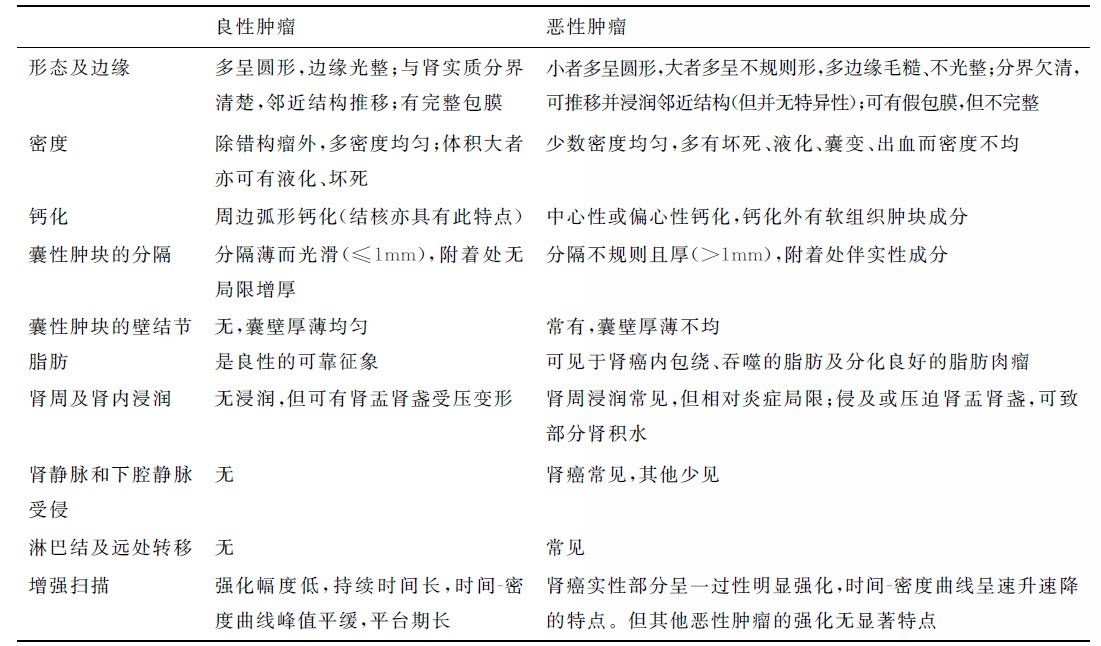
\includegraphics[width=\textwidth,height=\textheight,keepaspectratio]{./images/Image00335.jpg}
\end{table}

\subsubsection{输尿管肿瘤}

输尿管原发肿瘤很少见,约75%~80%属恶性。良性肿瘤有乳头状瘤和血管性息肉等。恶性肿瘤较良性肿瘤多见,其中85%为移行细胞癌,15%为鳞癌。因管壁较薄,又有丰富的淋巴管网和毛细血管网,故癌肿易突破管壁形成局部转移,亦可远处转移。

\subsubsection{膀胱肿瘤}

膀胱肿瘤以恶性多见。绝大多数膀胱肿瘤来自膀胱黏膜即移行上皮,如良性的乳头状瘤和恶性的移行上皮癌。还有少数的鳞癌和腺癌。乳头状瘤潜在恶变,术后极易复发,应视为低度恶性肿瘤。以上肿瘤占膀胱肿瘤的95%以上。

少见的有来自中胚层的肿瘤,如良性的平滑肌瘤、纤维瘤、神经纤维瘤、血管瘤、嗜铬细胞瘤、肾源性腺瘤;恶性的如平滑肌肉瘤、淋巴瘤等成人多见,儿童可见横纹肌肉瘤、畸胎瘤、皮样囊肿、错构瘤等。

膀胱肿瘤可为上泌尿道的肿瘤种植。

\subsection{肾血管平滑肌脂肪瘤}

本病又称为错构瘤、良性间叶瘤,是最常见的肾良性肿瘤。

\textbf{【病理】}
一般起源于肾实质,也可起源于肾窦、肾包膜或肾周连接组织。肿瘤大下不等,可达10cm以上。肿瘤界限清楚,但无包膜。其组织成分主要包括成熟的血管、平滑肌和脂肪组织。肿瘤血管丰富,可有出血、坏死、囊变和钙化。

\textbf{【临床表现】}
本病可多年无症状,典型表现为腰痛、血尿和腹部包块。其中腰痛最多见,血尿少见,腹部包块罕见。结节性硬化者则出现相应临床表现。

该病可分为两种类型。①单纯的肾错构瘤、不合并结节性硬化症:单侧单发为主,两侧同时发生约5%~10%。好发于40~70岁,女性多见。②伴结节性硬化症:常为多发,两侧性。大约20%肾错构瘤伴有结节性硬化症,而结节性硬化症的病例50%~80%伴有肾错构瘤。多发生于中青年。

\textbf{【CT表现】}
本病含有脂肪是其特征性的病理表现,准确地显示脂肪成分是其诊断的关键,即使少量也具有诊断意义,故必要时应薄层扫描(图\ref{fig15-19})。CT表现为肾实质内境界清楚的占位性病变,密度不均匀;亦可位于肾周或包绕肾脏。增强扫描部分瘤组织强化,尤其是血管组织,但脂肪组织和坏死区不强化。极少数以平滑肌为主者呈软组织密度,难与肾癌鉴别。本病有出血倾向(尤其较大者),出血可掩盖脂肪成分;也可伴肾包膜下、肾周和(或)腹膜后出血,产生大量纤维化。巨大的错构瘤可恶变,但少见。

\begin{figure}[!htbp]
 \centering
 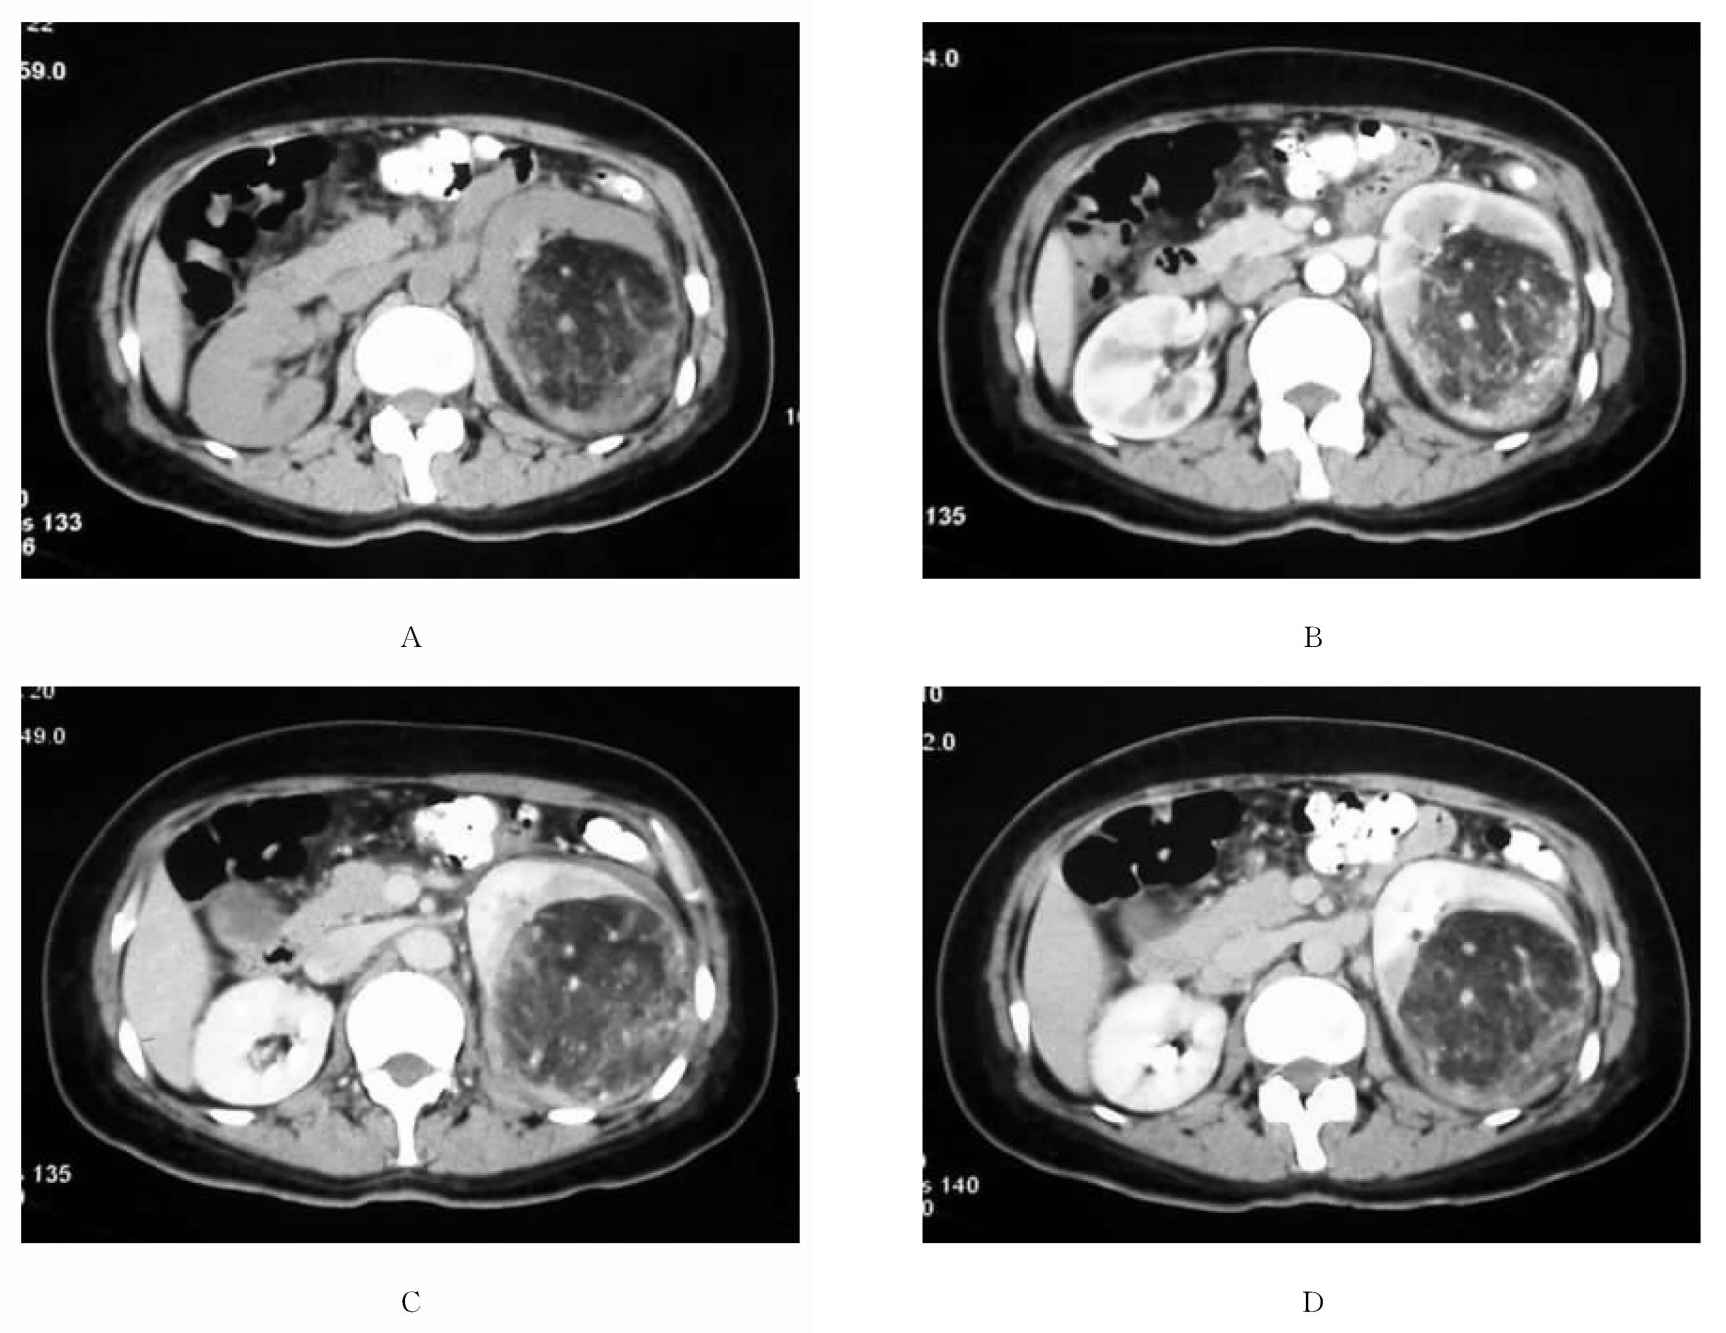
\includegraphics[width=.7\textwidth,height=\textheight,keepaspectratio]{./images/Image00336.jpg}
 \captionsetup{justification=centering}
 \caption{左肾错构瘤\\{\small A为平扫,B为皮质期,C为实质期,D为肾盂期。平扫左肾内有巨大低密度灶,其内含有大量脂肪,以及条索状、结节状稍高密度灶;增强扫描其内条索状、结节状结构强化较著,脂肪组织无强化}}
 \label{fig15-19}
  \end{figure} 

有学者认为,乏脂肪者呈均一强化和持续强化为其CT特点,有别于肾癌速生速降的强化特点。

\textbf{【鉴别诊断】}
①脂肪瘤和脂肪肉瘤:脂肪瘤和分化良好的脂肪肉瘤CT表现为有间隔、境界清晰的脂肪密度肿块,且脂肪瘤无强化,多可与错构瘤相鉴别。分化不良的脂肪肉瘤表现类似恶性肿瘤,有侵蚀性,密度与软组织类似,不难鉴别。②肾癌:肾癌内脂肪成分罕见,多为肾癌侵犯、包绕或吞噬脂肪所致,注意分析多可鉴别。两病可同时存在,应予注意。此外,肾畸胎瘤罕见,容易诊断。

\subsection{肾腺瘤}

肾腺瘤为良性肾肿瘤,但一般认为是一种潜在恶性的肿瘤或癌前病变。无论病理还是影像学与肾癌均难以区别。

\textbf{【病理】}
肿瘤多<3cm,生长缓慢,常为尸检时偶然发现。腺瘤多位于靠近包膜的肾皮质处,生长甚慢,界限清楚。组织学上分3类:乳头状型、管状型和腺泡型。6%的肾癌起源于肾腺瘤。

\textbf{【临床表现】}
多无症状,而偶尔发现。因少数肾癌起源于腺瘤,故临床应作为早期癌瘤对待。

\textbf{【CT表现】}
肾实质内圆形等密度或稍高密度结节,多<3cm,边缘清楚,可有钙化。增强扫描轻度强化,有细分隔或呈网格状。有时增强曲线酷似肾癌。

总之,本病与小肾癌及其他良性肿瘤均难以鉴别。

\subsection{肾嗜酸细胞瘤}

本病又称为肾嗜酸细胞腺瘤,是一种少见的有别于肾腺瘤的良性肿瘤。嗜酸细胞瘤属于上皮来源,可起源于肾、唾液腺、甲状腺、胸腺等,也有肾上腺的报道。

\textbf{【病理】}
多为单发,偶为多发、两肾发病。肿瘤大小0.6~15cm不等,平均4.4cm。肿瘤质地较均匀,中心有瘢痕(54%可见),通常认为瘢痕是由于肿瘤缓慢生长、长期缺血所致,故肿瘤越大其发生率亦越高。但无出血、坏死。光镜下肿瘤细胞呈单一性,胞浆嗜酸颗粒丰富,偶尔可见核的多形性,核仁明显;电镜下胞浆内充满紧密排列的肿胀线粒体。此病的生物学行为,文献争论较多。一方面虽为良性,但有潜在恶性行为。另一方面又有人将其分为3级:Ⅰ级为良性;Ⅱ级有潜在恶性倾向;Ⅲ级为恶性。但亦有人认为不存在恶性可能。

\textbf{【临床表现】} 通常无症状,少数有腰痛、血尿或腹部包块。

\textbf{【CT表现】}
①平扫呈等密度或稍高密度肿块,界限清楚。②增强扫描呈中度强化,而表现为相对低密度(低于肾强化幅度),无坏死囊变、出血。③中心星状瘢痕:是本病的特征性表现,呈长条状或星状低密度。④肿瘤内的钙化:少见。⑤肿瘤包膜:平扫呈等密度常不易显示;增强扫描有助于显示,可呈稍高密度。

\textbf{【鉴别诊断】}
①肾癌:肿瘤密度不均,常有坏死出血,甚至呈囊性肿块,边缘多欠清晰,包膜不完整。而嗜酸细胞瘤密度多较均匀,中心可有条状或星状低密度瘢痕,无坏死囊变、出血。②肾腺瘤:通常<3cm,其密度多均匀,边缘清晰。两者多难以鉴别,但肾腺瘤无中心瘢痕。③肾血管平滑肌脂肪瘤:含有脂肪者不难鉴别,但小者且缺乏脂肪时则难以区分。

\subsection{肾球旁细胞瘤}

本病又称为肾素瘤,是一种良性肾素分泌性肿瘤。由肾小球入球小动脉的平滑肌细胞分化而来,极其罕见。

\textbf{【病理】}
肿瘤位于肾皮质内,界限清楚,瘤内常有出血灶。组织学上为单一细胞组成,排列成巢索状或管状结构,其间有许多血管间隙。肿瘤细胞可有许多分泌颗粒,与正常肾小球球旁细胞特点一致。

\textbf{【临床表现】}
多发生于15~20岁,女性多见。有严重的持续性高血压、头痛、烦渴、多尿、夜尿增多以及低血钾症状。实验室检查以血醛固酮水平增高、肾素升高、低血钾为特征。常合并多次脑出血症状及征象。也可无症状。

\textbf{【CT表现】}
肿瘤一般单发、较小,2~5cm。肿瘤位于肾皮质处,偶尔位于肾皮质下或肾周间隙。病灶呈等、低密度,边缘光整。因相对乏血增强扫描呈轻度强化,而仍低于肾实质。此外患者可有反复脑出血表现。

总之,结合其典型的临床表现及CT特点,该病的诊断准确性高。但需注意与分泌肾素的肾细胞癌、肾腺瘤鉴别。

\subsection{肾血管瘤}

本病罕见,是累及血管的先天性肿瘤样病变。

\textbf{【病理】}
多为单侧,可累及肾皮质、髓质或肾盂的上皮下区,大多位于髓质。病变一般较小,有的可达10cm以上。与其他部位的血管瘤相似,可为毛细血管型或海绵状型,多为海绵状。由充满血液和血栓的海绵状薄壁血管构成,可有退化、坏死后充满血液的大囊腔。

\textbf{【临床表现】}
大多无症状。部分患者可有血尿,可为持续性,大多为间歇性;伴疼痛及血块。重者大出血伴腰痛。

\textbf{【CT表现】}
平扫血管瘤呈等密度(因肝、脾密度高于肾脏,故肾血管瘤呈等密度)。增强扫描病变呈多发结节状、团块状强化,且持续时间较长为其典型表现。有时可见迂曲成团的血管。

\textbf{【鉴别诊断】}
主要与肾癌鉴别。肾癌呈低密度,常有出血、坏死、囊变,而无结节状、团块状强化,可资鉴别。

\subsection{肾囊性淋巴管瘤}

本病为罕见的肾脏良性肿瘤,术前诊断困难。

\textbf{【病因病理】}
其发生与淋巴组织发育不良导致继发的淋巴管扩张有关。病灶大小与淋巴管梗阻的位置有关。如果经过肾蒂的淋巴管阻塞,可引起双肾弥漫性淋巴囊肿;如肾内小的淋巴管阻塞,则可引起局限性肿块或淋巴囊肿。

\textbf{【临床表现】}
可发病于所有年龄,多在30岁以后。血尿、腰部钝痛、肾绞痛及肾部肿块为最常见的表现。

\textbf{【CT表现】}
常表现为被膜下或肾内低密度肿块,肾大小多无改变。平扫为圆形或类圆形低密度灶,边界清楚,密度均匀,可单发或多发;或弥漫分布于肾周呈环形均匀密度,边界清楚。因阻塞淋巴管进行性扩张,故显示多腔病变、分隔厚薄不均。偶于肿瘤边缘见有钙化。增强扫描多无强化,部分有轻度强化。亦可由于肾小管及血管的强化,其内见散在扩张的淋巴管。

\subsection{其他少见肾良性肿瘤}

\subsubsection{肾平滑肌瘤}

常位于包膜下的肾皮质内,一般仅数毫米大小。

\textbf{【CT表现】} 无特异性,呈低密度结节;增强扫描有强化。

\subsubsection{肾纤维瘤}

肿瘤一般甚小,多位于髓质,少数位于皮质,具有完整包膜。单发多见,偶为多发且可累及双肾。多无症状。

\textbf{【CT表现】}
无特异性。平扫呈高密度,密度均匀,多无坏死囊变,可有钙化骨化表现;增强扫描为乏血性肿块,但可延迟强化。

\subsubsection{弥漫性肾胚细胞瘤病}

本病少见。本病累及肾皮质全层,肾脏增大,胚胎小叶显著。常见于肾母细胞瘤患者,尤其是两肾肾母细胞瘤者,因此认为是肾母细胞瘤的前期病变。

\textbf{【CT表现】}
无特异性。表现为肾显著增大,肾盂、肾盏伸展、扭曲;一侧肾或双肾多发不强化的低密度灶,有假包膜。对<2~3mm者不易检出。

\subsection{肾细胞癌}

肾癌又称肾细胞癌,起源于肾小管或集合管的上皮细胞,为泌尿系最常见的恶性肿瘤,约占肾恶性肿瘤的85%。

\textbf{【病理】}
肿瘤94%以上呈膨胀性生长,没有包膜,但可以有假包膜(由肾组织受压变性、纤维化而形成)。瘤内常发生出血、坏死、囊变、钙化甚至纤维化。1997年国际抗癌联盟和美国癌症联合会推荐使用新分型法分为5种亚型:透明细胞癌(约占70%)、乳头状癌(又称嗜色细胞癌,约占10%~18.5%)、嫌色细胞癌(约占4%~5.9%)、集合管癌(约占0.4%~3%)及未归类肾癌。透明细胞癌起源于肾近曲小管,肿瘤血管丰富,常同时含有实性和囊性结构,极少数以囊性为主。乳头状癌起源于肾近曲小管或远曲小管,肿瘤常有出血、坏死、囊变及明显纤维包膜。嫌色细胞癌起源于肾集合管的暗细胞,肿瘤一般呈实性结构,很少出血坏死。

本病5%为多灶性,1%~2%为两侧性。其转移途径为局部浸润、淋巴转移和血行转移。小肾细胞癌是指肿瘤直径≤3.0cm的肾癌,这种癌肿常认为是早期病变。

囊性肾细胞癌占肾细胞癌总数的10%~15%。其形成机制尚不清楚,可能与下列因素有关。①肿瘤呈囊性生长,形成大小不等、互不相通的多房囊性肿物,常有假包膜。②肾癌中心供血不足,出血和坏死囊变。其壁厚且不规则,常为单房。③肾癌起源于囊肿壁上的上皮细胞,结节常位于囊肿的基底部。④肾癌引起肾小管或肾小动脉阻塞导致囊肿形成,当肿瘤增大时,嵌入囊肿内,此型少见。

\textbf{【临床表现】}
好发于40~70岁,男女之比约为2∶1,罕见于青年或儿童。早期多无症状,随病情发展可出现3大症状。①40%~80%出现无痛性血尿;②30%~60%有腰痛,多为钝痛,血块通过输尿管出现绞痛;③20%~40%触及腹部包块。此外,小肾癌临床无症状,及时切除预后甚佳。

\textbf{【CT表现】}

\subsubsection{常见表现}

其常见表现为:①平扫呈形态不规则的软组织肿块,常使肾外形扩大或局部隆起(图\ref{fig15-20})。有短毛刺并与肾周筋膜相连是其主要指征之一。多边界清楚。有时平扫显示不清,只有增强扫描才能发现。病灶内常有囊变、出血、坏死、钙化等,少数可合并感染。瘤内出血表现为高密度灶;钙化呈中心性或偏心性,钙化外有软组织成分(而良性钙化多为边缘性)。②增强扫描:大部分肾癌为多血供型,在增强早期(皮髓交界期)病灶明显强化,CT值升高多>20Hu,随后快速下降,即强化曲线呈速升速降的特点(图\ref{fig15-21})。约在30~40s以后开始转为低密度。少血供者强化不著。增强扫描还可观察肾静脉内或下腔静脉内有无癌栓存在,主要表现为在增强血管腔内的低密度占位表现,并可见因血管受侵而局限扩张。③大多数肾癌向内可压迫、侵犯甚至填塞肾盂、肾盏,部分可有肾积水征象。向外可突破肾包膜侵入肾周脂肪和肾筋膜,表现为肾周脂肪层模糊、消失,肾筋膜增厚,但上述并非肿瘤侵犯的特异征象,如出现包膜外壁结节或肾周间隙内肿块,则可肯定包膜或肾周间隙受侵。④淋巴结转移:淋巴结≥1.5cm应考虑转移,而<1.0cm则为正常范围,1.0~1.5cm之间者不易定性。⑤远处血行转移:最常见于肺、骨、肝。

\begin{figure}[!htbp]
 \centering
 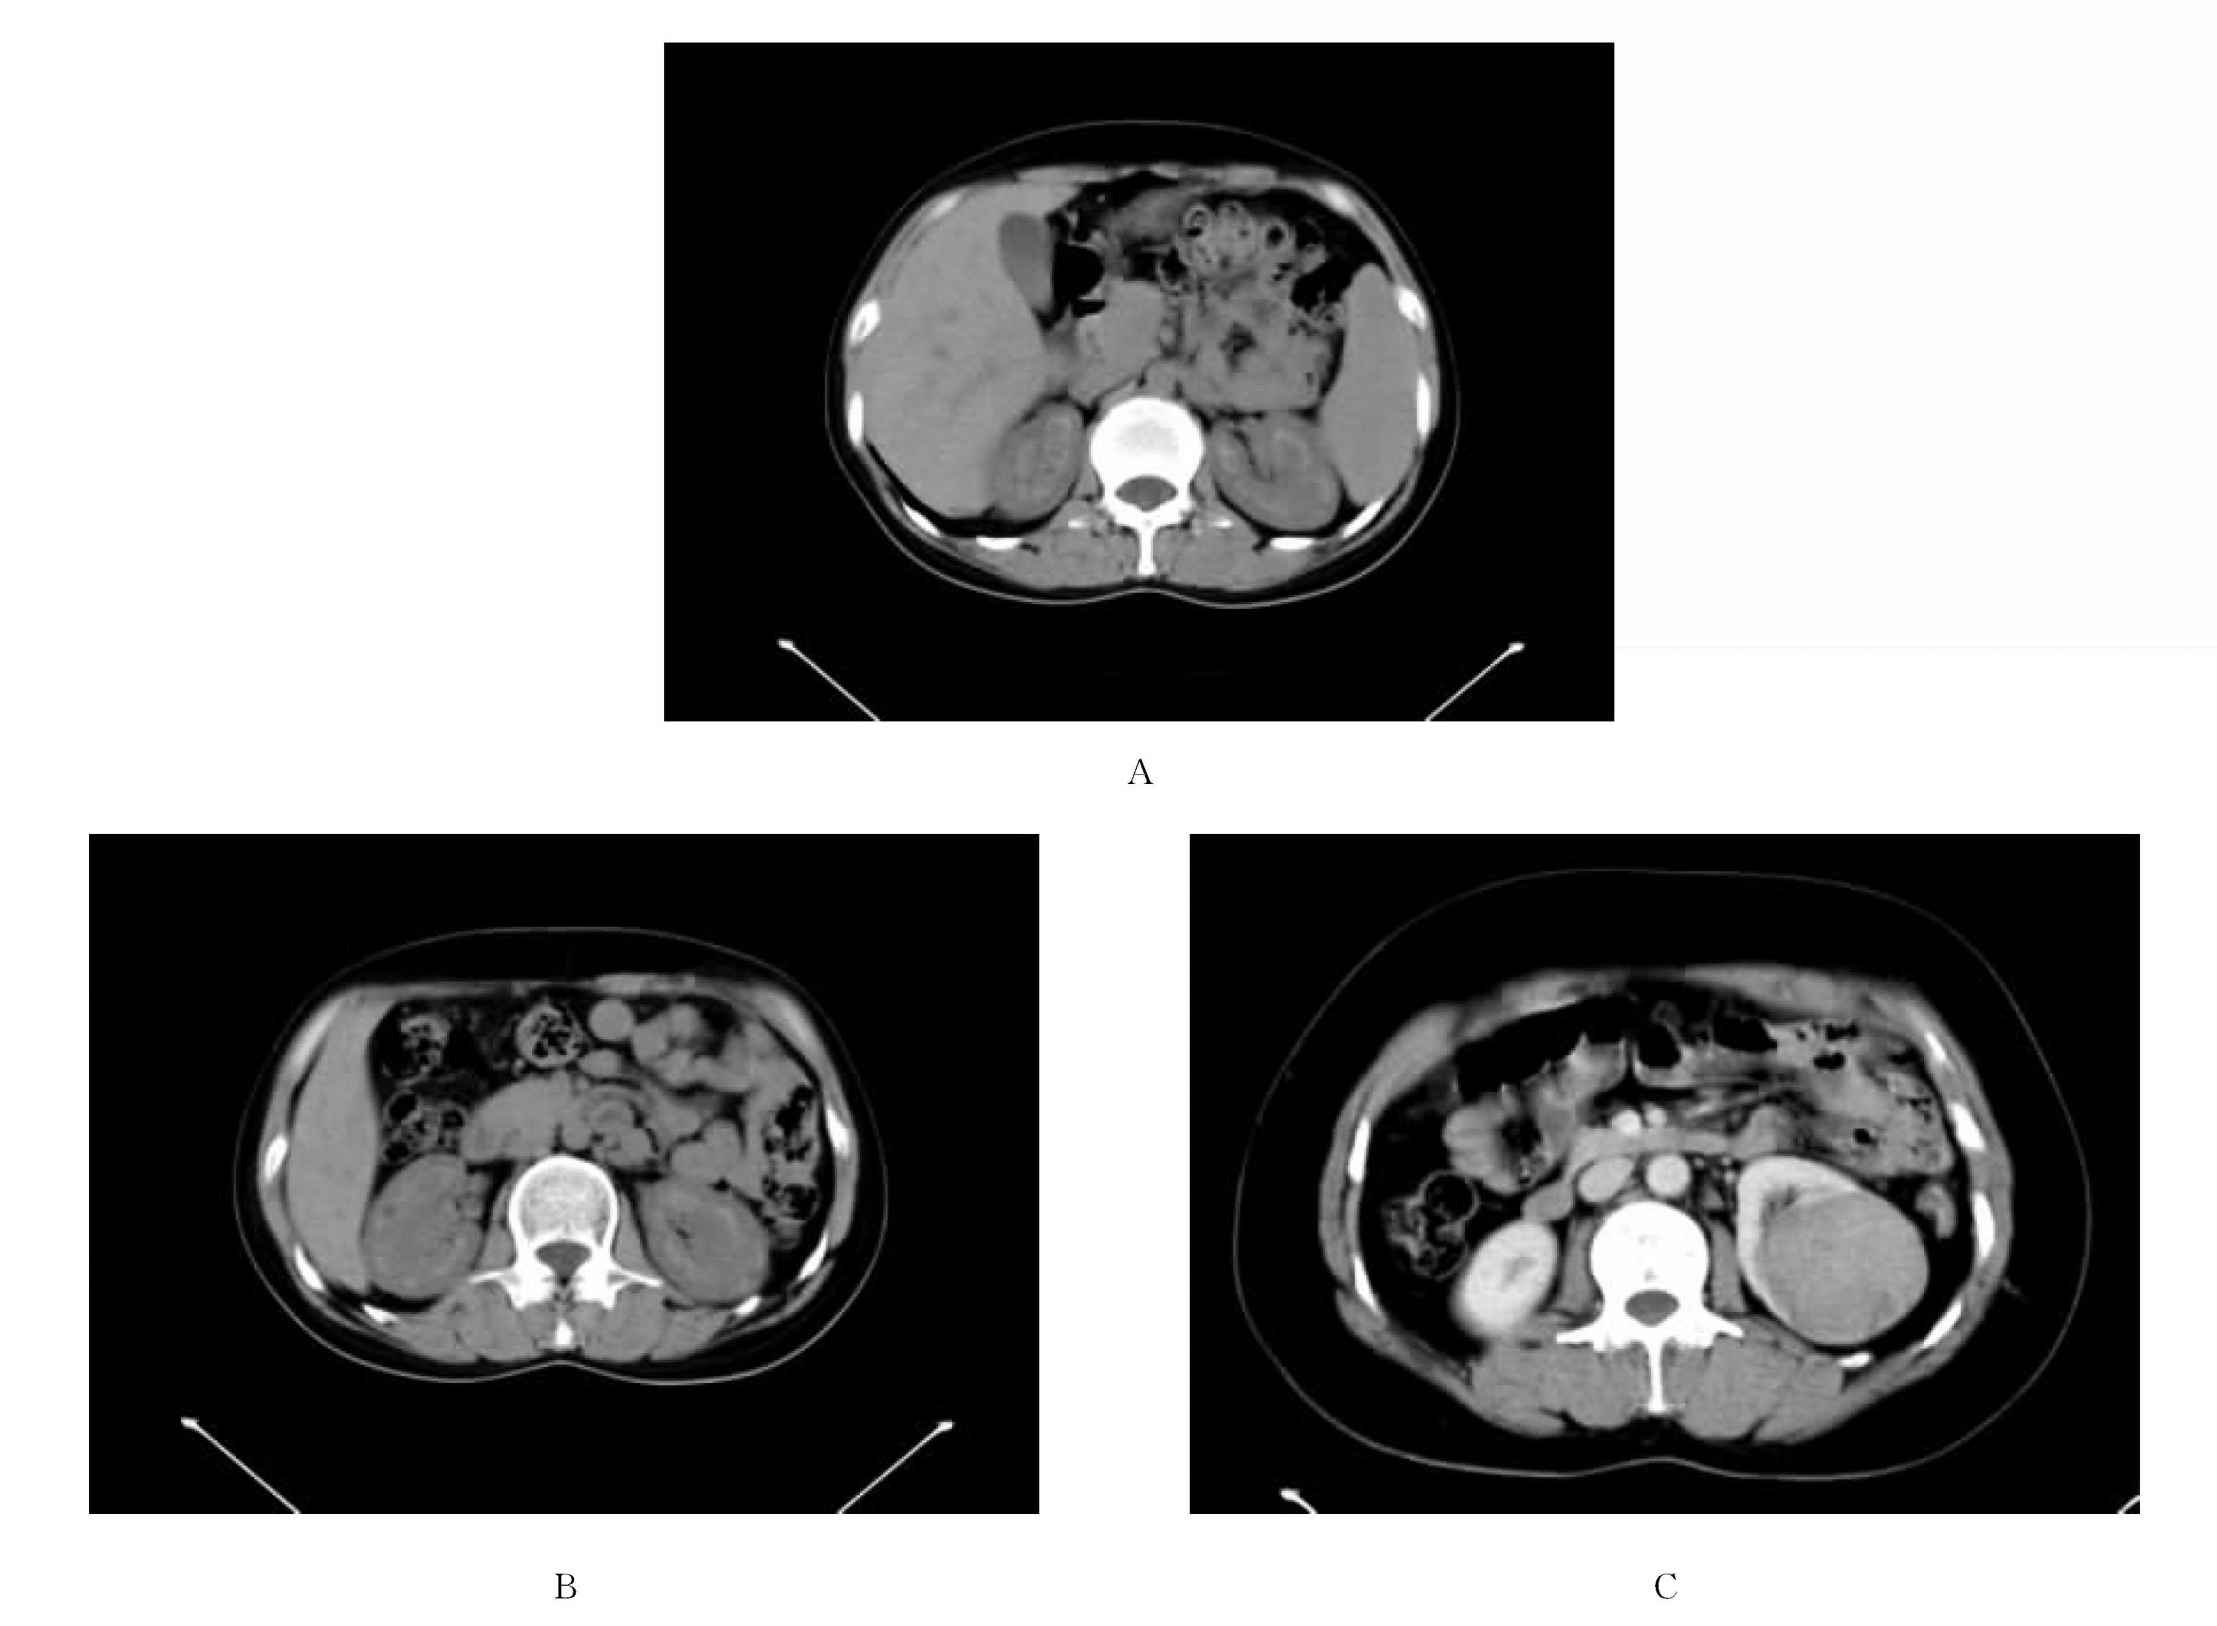
\includegraphics[width=.7\textwidth,height=\textheight,keepaspectratio]{./images/Image00337.jpg}
 \captionsetup{justification=centering}
 \caption{左肾癌\\{\small A为平扫病灶呈等密度;B为皮质期呈高密度强化;C为实质期密度低于肾实质}}
 \label{fig15-20}
  \end{figure} 

\begin{figure}[!htbp]
 \centering
 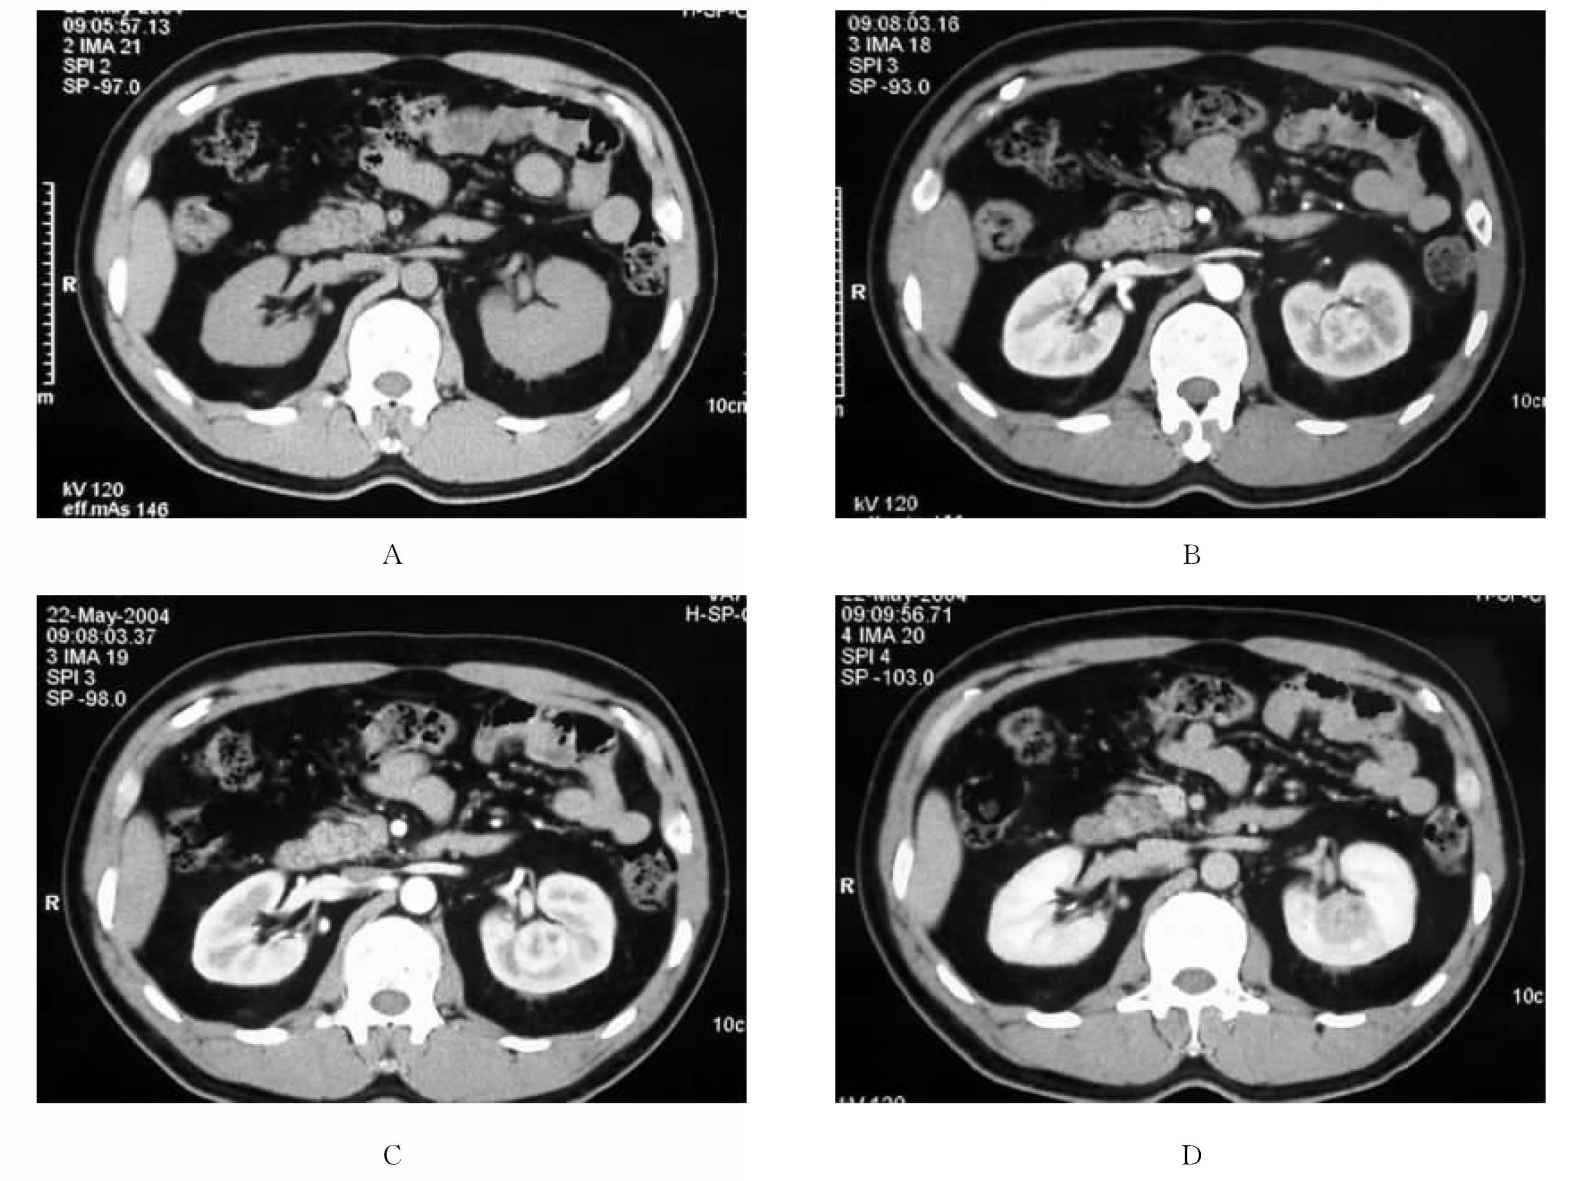
\includegraphics[width=.7\textwidth,height=\textheight,keepaspectratio]{./images/Image00338.jpg}
 \captionsetup{justification=centering}
 \caption{左侧小肾癌\\{\small A为平扫病灶呈等密度,界限不清;B、C为皮质期呈高密度强化;D为实质期密度快速下降}}
 \label{fig15-21}
  \end{figure} 

国外有学者认为,皮髓交界期明显强化只出现在透明细胞癌(75%),而不出现在其他类型细胞癌;并且还有学者认为,皮髓交界期CT值>83.5Hu,排泄期CT值>63.5Hu,很可能是透明细胞癌。国内有学者发现,在皮髓交界、实质和排泄期透明细胞癌比乳头状癌和嫌色细胞癌强化明显(图\ref{fig15-22})。

\begin{figure}[!htbp]
 \centering
 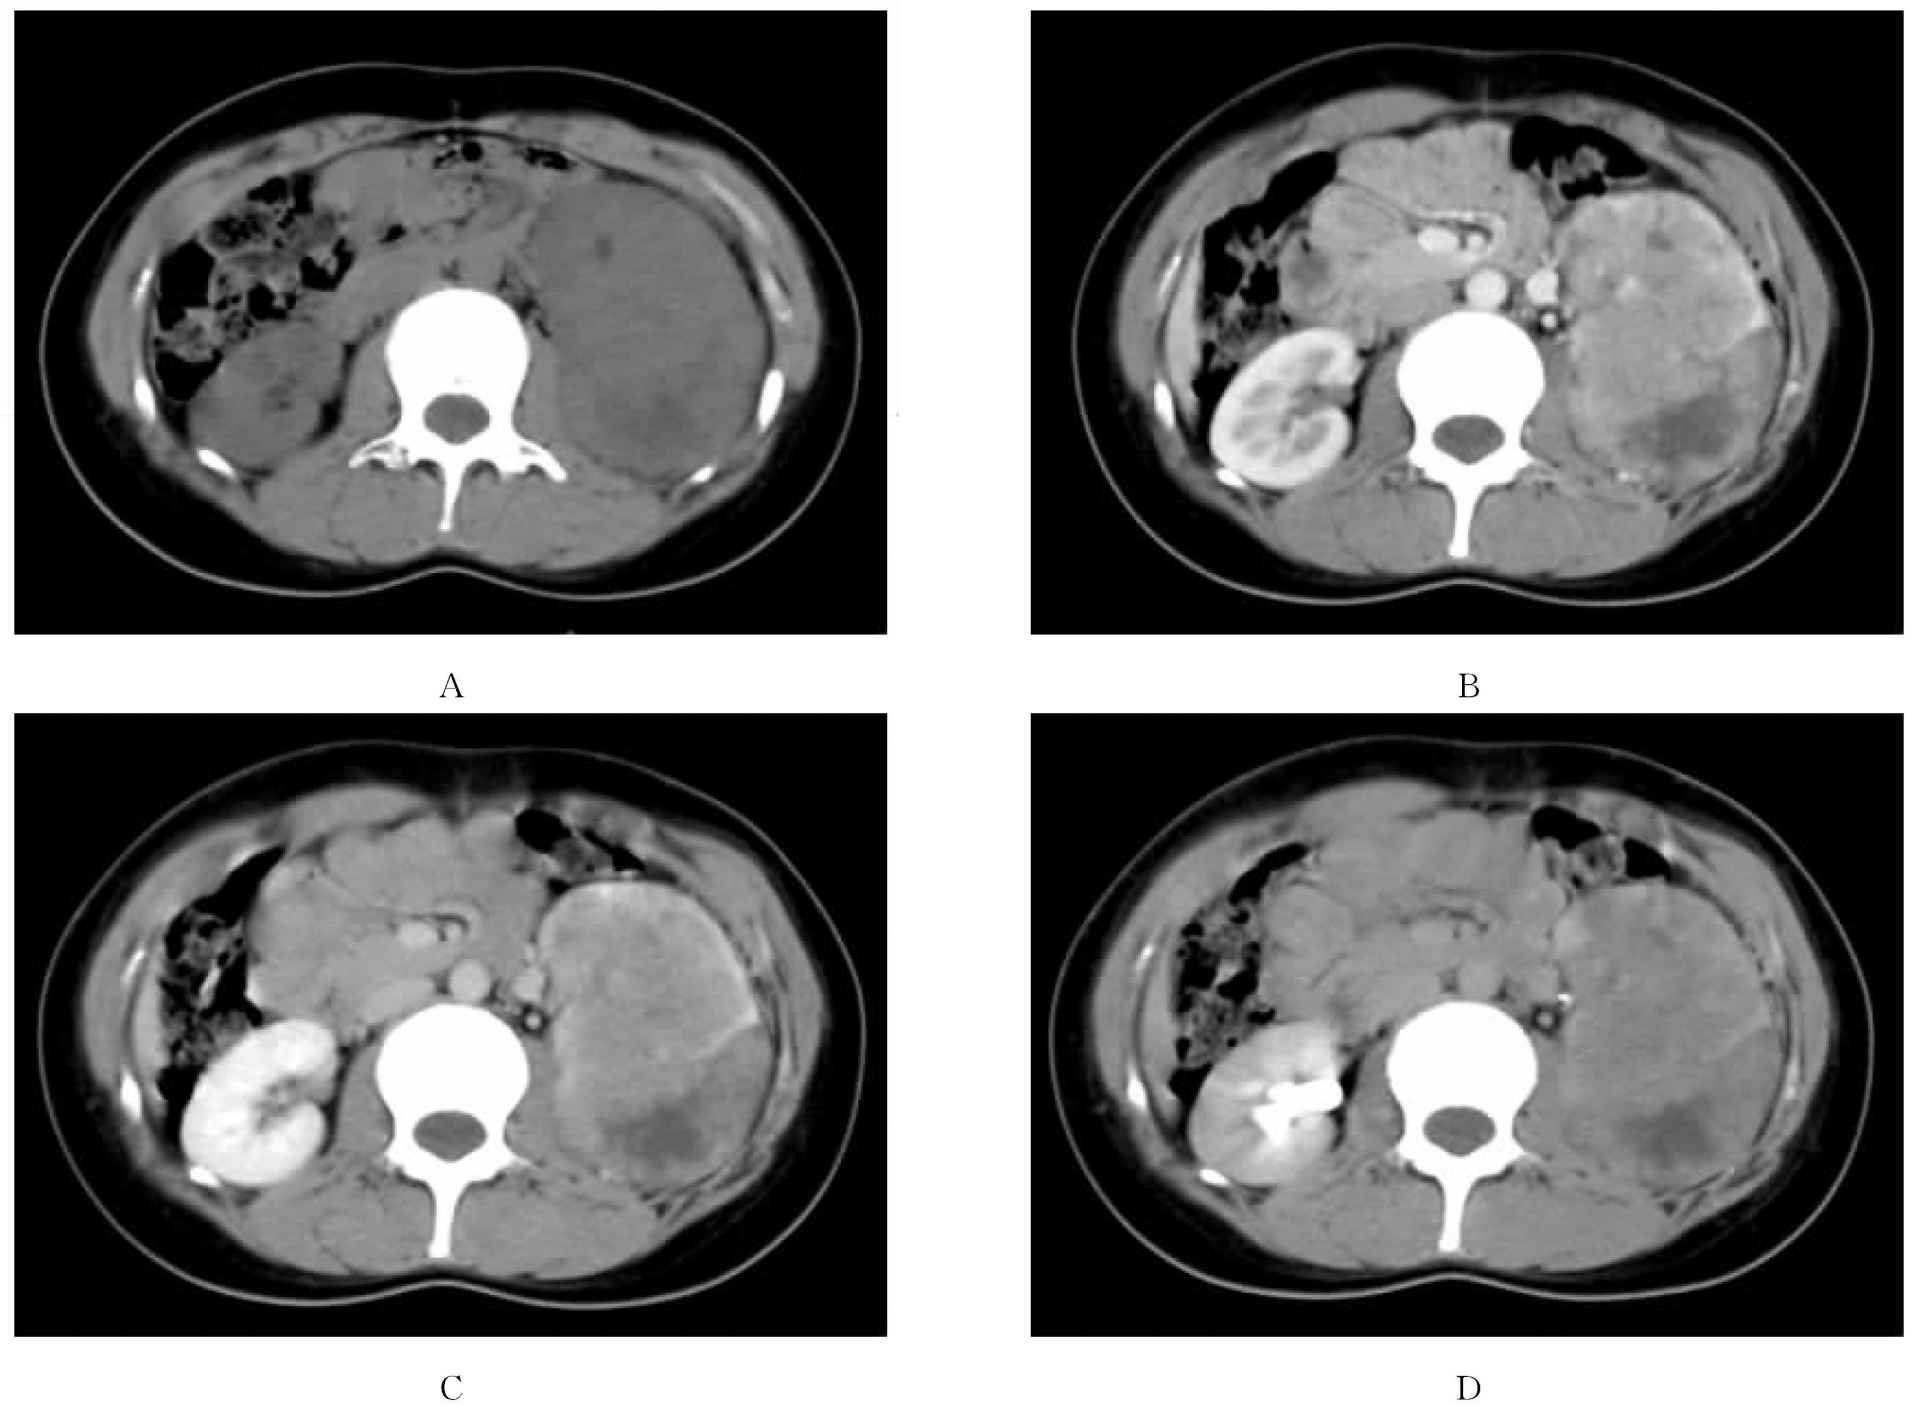
\includegraphics[width=.7\textwidth,height=\textheight,keepaspectratio]{./images/Image00339.jpg}
 \captionsetup{justification=centering}
 \caption{肾乳头状癌\\{\small A~D分别为平扫、皮髓交界期、实质期和排泄期,肿瘤强化相对不显著}}
 \label{fig15-22}
  \end{figure} 

\subsubsection{肾细胞癌边缘部CT征象与病理表现的关系}

肿瘤边缘的3类CT形态恰与病理上肿瘤边缘的3种类型相对应。①CT肿瘤边缘清楚无分叶者,病理上大多包膜完整;②边缘清楚伴分叶者,病理上大多包膜不完整或锯齿状;③边缘不清者,病理上大多无包膜。

平扫肿瘤边缘不清者,增强后肿瘤大多“缩小”或边缘变清。边缘不清是肿瘤周围正常肾实质内散在浸润的癌细胞所致。平扫肿瘤边缘清楚,无论有无分叶,癌细胞分化程度较高;而边缘不清者,癌细胞分化程度较低,呈浸润性生长。

\subsubsection{小肾细胞癌}

小肾癌是指肿瘤直径≤3.0cm的肾细胞癌。大多呈圆形或椭圆形,密度均匀,平扫时低于或等于肾实质,约在30~40Hu之间;少数因出血而密度较高,边缘多较清楚;少数密度不均,界限也欠清。可突出肾轮廓外。肿瘤内可有出血、坏死、囊性变,但钙化少见。增强扫描因大多数血供丰富,而在皮质期明显强化,CT值增加40Hu以上,实质期强化迅速减退,呈“速升速降”表现(图\ref{fig15-21})。增强后密度不均是由于瘤内多有出血、坏死、囊性变所致。小囊性肾癌的囊壁、壁结节、囊内分隔也于皮质期明显强化,且呈“速升速降”表现。假包膜发生率很高,但CT只能发现少部分。

总之,小肾癌可无轮廓异常,多有假包膜形成而边缘清楚、密度可不均、速升速降型强化曲线是其较为特征性的表现。少血供型难以定性,需注意与良性肿瘤甚至出血性肾囊肿鉴别。

\subsubsection{囊性肾细胞癌}

CT表现为:①囊壁改变:囊壁较厚,且不均匀、不规则。增强扫描可见囊壁、分隔及结节的早期厚环状不规则强化和“快进快退”的特点。②钙化:囊壁及分隔钙化明显,呈斑点状、线条状及壳状,且广泛粗大,有别于线形、量少、薄而细的良性钙化。③分隔:常见,且粗细不均,通常>1mm,与囊壁交界处呈结节状增厚。④囊液:密度不均,可出现碎屑、凝血块等。⑤病变与正常肾实质的分界:多不清,与缺乏包膜及浸润性生长有关。⑥病变的大小:常较大。当较小时,恶性征象少或不明显,则诊断困难。⑦鉴别诊断:应注意与肾囊肿并感染、肾畸胎瘤、肾结核、多囊肾等囊性病变相鉴别。此外,肾盂癌、肾母细胞瘤亦可呈囊样生长。

总之,肾癌应注意结合病史与弥漫性黄色肉芽肿性肾盂肾炎、肾脓肿及肾周脓肿,以及淋巴瘤、脂肪肉瘤等相鉴别。

\subsection{肾脏集合管癌}

本病又称Bellini导管癌,是恶性程度较高的上皮细胞性肿瘤,因起源于集合管上皮细胞而得名,约占肾癌的0.4%~3%。

\textbf{【病理】}
虽然肾皮质和髓质中均可见到集合管,但肉眼观察集合管癌位于髓质。也有学者根据肿瘤浸润的部位不同分为单纯髓质型、皮质髓质型和皮质-髓质-肾盂型。该肿瘤有向肾内、外浸润及淋巴结转移和远处血行转移的特点。组织学特点是瘤细胞呈腺管状或腺管乳头状排列,内有明显间质反应及淋巴细胞、浆细胞、其他炎性细胞浸润;免疫组织化学检查肿瘤细胞表达34BE12和(或)PNA等。

\textbf{【临床表现】}
多见于青壮年,发病年龄为20~80岁,男性略多。血尿、腰腹痛为最常见的症状。还可有腹胀、腹块以及远处转移的症状。

\textbf{【CT表现】}
肿瘤较小时,表现为髓质区界限不清的低密度灶,肾轮廓无改变;中度均匀强化。肿瘤较大时,累及肾皮质并侵犯肾被膜及周围结构时,表现为界限不清的混杂密度灶,可有囊变、坏死及钙化;增强扫描强化不均,肾盂及肾盏受压移位;肿瘤突破肾被膜则可肾周脂肪囊密度增高、条索状影及肾筋膜增厚;同时,还可见肾盂软组织块、肾窦脂肪密度消失,以及肾动、静脉受累。

\textbf{【鉴别诊断】}
主要应与肾透明细胞癌鉴别,后者肿瘤界限多清楚,肾被膜、肾周脂肪囊、肾筋膜的受累相对少见。尤其增强扫描无论在皮质期、实质期,还是肾盂期,其肿瘤实性部分的强化程度总是高于肾集合管癌,有助于鉴别。此外,结合肾盂癌的生长部位和生长特点,两者也可鉴别。但肾集合管癌的确诊及鉴别仍靠病理组织学。

\subsection{肾盂癌}

肾盂癌占肾恶性肿瘤的8%~12%。肾盂癌较单纯输尿管癌多2~3倍,而膀胱癌50倍于肾盂原发癌。

\textbf{【病理】}
肾盂癌约85%~95%为移行细胞癌,此外,还有10%为鳞状细胞癌,腺癌不到1%。移行细胞癌最常发生于肾盂(82%~90%),且常为多发(20%~44%);同时发生在膀胱10%,同侧输尿管17%,或同时发生在膀胱和输尿管(15%)。85%的移行细胞癌是乳头型,属低度恶性,浸润慢、转移晚。非乳头型移行细胞癌为浸润性恶性病变,恶性程度高,早期可直接扩散和转移,5年生存率小于10%。

此外,所谓的良性乳头状瘤,易恶变,亦有学者认为属低度恶性,影像学难以鉴别。

肾盂癌的转移途径:①局部浸润肾实质、肾盂和肾门周围组织。②淋巴转移:主动脉旁、纵隔和锁骨上淋巴结转移。③血行转移:肺、肝和骨多见,其次为肾上腺、对侧肾和胰、脾。

\textbf{【临床表现】}
好发于40岁以后,以50~70岁多见,男女之比(2~3)∶1,典型症状为无痛性、间歇性全程血尿。腰痛以钝痛为主,血块进入输尿管可出现绞痛。

\textbf{【CT表现】}
表现为肾盂内软组织肿块,CT值约8~30Hu,密度高于尿,低于肾实质。典型的肾盂移行细胞癌常居肾盂的中央,且常呈离心性膨胀性生长,可侵犯肾窦及肾实质,但肾外形多不发生变化,为其特点之一。若肿瘤侵犯大部肾脏或蔓延至肾外时,其表现可类似肾细胞癌。肾盂癌血供少于肾细胞癌,增强扫描可轻、中度强化,肾功能常减退(图\ref{fig15-23})。但我们遇见1例于实质期呈显著强化,CT值升高近80Hu。晚期患者,延迟扫描有时可见未累及的散在肾实质呈条带状轻度或明显强化。少数可有钙化(约占1%),呈散在或集中的不规则高密度钙化灶。还可有肾小盏或肾盂变形、受压、移位、梗阻,甚至发生肾盂肾盏积水。非乳头状移行细胞癌及鳞癌很少或不产生肾盂内低密度光滑的或分叶状软组织肿块,但可有管壁增厚、浸润性肾肿块表现。

\begin{figure}[!htbp]
 \centering
 
\includegraphics[width=.7\textwidth,height=\textheight,keepaspectratio]{./images/Image00340.jpg}
 \captionsetup{justification=centering}
 \caption{右肾盂癌\\{\small A为皮质期,B为实质期,C为肾盂期;右肾盂区有软组织密度灶,增强扫描轻度强化;右肾盂肾盏有积水表现}}
 \label{fig15-23}
  \end{figure} 

\textbf{【鉴别诊断】}

1.肾细胞癌:当肾癌和肾盂癌长到一定大小时,均可向肾盂和肾实质方向相互侵犯,而鉴别困难,下列特点有助于鉴别。①肾癌血供丰富,增强比肾盂癌明显。②肾盂癌常居于肾盂中央,且常呈离心性生长增大和(或)浸润肾实质;肾癌则起源于外周肾实质,甚至起源于中央者,也偏心侵犯肾窦。但晚期这种关系不复存在,而鉴别困难。③即使很大的肾盂癌,仍可保持肾外形轮廓不变,这种情况在肾癌中少见。④晚期肾盂癌倾向于造成收集系统阻塞,使肾功能部分或几乎完全丧失;延迟扫描未累及的小部分散在肾实质呈条状强化,提示肿瘤中心性起源、离心性扩张或侵犯。⑤即使晚期肾盂癌也很少侵犯肾静脉和下腔静脉。

2.结石、凝血块、肾盂旁囊肿:平扫CT值肾囊肿为-10~10Hu、结石为100~250Hu、凝血块一般为50~65Hu,而肾盂癌多为8~30Hu;且前三者增强扫描均无强化。藉此多可鉴别。

\subsection{肾母细胞瘤}

本病又称为肾胚胎瘤或Wilms瘤,系恶性胚胎性混合瘤。约占肾恶性肿瘤的6%,是儿童期最常见的恶性肿瘤之一。可发生于肾的任何部位,但始自肾盂者少见。

\textbf{【病理】}
本病起源于间胚叶组织,由胚芽、上皮、间叶三种成分构成,后者可化生为肌肉、脂肪、血管、软骨和骨组织等。肿瘤多单发,也可多中心起源,4%~10%为双侧性。肿瘤大多位于肾包膜下肾皮质,外生型主要向肾外生长。而所谓肾外型罕见,主要起源于肾异位的胚细胞,多位于肾脏附近腰椎旁,亦可位于腹股沟、盆腔、后纵隔等。肿瘤内可有坏死、囊变、出血和钙化。肿瘤增大可直接侵犯或挤压肾组织,引起肾盂、肾盏的变形,并突破肾包膜侵入肾外组织。少数侵及肾盂输尿管,可种植到远处泌尿器官。30%~40%侵及肾静脉及下腔静脉。常转移到肺、肝,腹膜后次之,骨、脑转移等少见。

\textbf{【临床表现】}
多见于1~3岁小儿,75%见于5岁以下,90%在7岁以前,新生儿极为罕见,男女发病相近。临床表现为腹胀或无痛性包块,少数有轻度腹痛、血尿(30%)、高血压、贫血、发热等。15%伴先天性畸形如先天性无虹膜、半身肥大、马蹄肾和内脏巨大症。

少数发生于成人的肾母细胞瘤,可发生于15~84岁,多见于20~30岁,女性稍多于男性。主要症状为迅速生长的腹部肿块,腹痛多位于腰、背部。就诊时间短,约一半以上有血尿,就诊时约1/3已有转移。

\textbf{【CT表现】}
肿瘤起自肾皮质,多位于一侧肾的上极(多于下极)。在肾内膨胀性或弥漫性生长,也可大部分向肾外膨隆而类似肾外肿瘤。平扫呈实性或囊实性肿块,少数以囊性病变为主。肿块密度不均,可有出血、坏死、囊变,较少有钙化(5%~15%,也有报道达27%)或低密度脂肪组织(7%)。瘤体一般较大,巨大者向前可抵腹壁、向内超越中线、向上下可压迫邻近脏器。残余的肾脏见于瘤体的周围或上下极内,平扫时与肿瘤分界不清。部分病例肿瘤内含有扩大的肾盂(盏),少数肿瘤早期经肾盏突入肾盂呈息肉状生长。增强扫描呈不均匀强化的实质性肿块,但仍低于明显强化的肾脏;肿瘤包膜可强化;肿瘤内出血、坏死、囊变区无强化而显示更清楚。在肾盂显影期可见肾盂、肾盏的受压、移位、变形和扩张等。国内有学者认为肿瘤压迫、侵蚀肾脏,使残存肾实质呈“新月形”强化,为肾母细胞瘤的典型CT表现,且此征象有助于与腹膜后其他恶性肿瘤侵及肾脏造成的破坏相鉴别。还可见肿瘤外侵、血管受侵、淋巴和远处血行转移表现。

成人肾母细胞瘤多位于肾包膜下的皮质部,因而常表现为自肾内向外延伸的肾外肿块。瘤内常有出血、坏死,并可有钙化,约75%有假包膜。增强扫描因少血管而轻度强化,肾静脉及下腔静脉内常有癌栓。

\textbf{【鉴别诊断】}

1.肾母细胞瘤主要应与神经母细胞瘤鉴别:肿块小时易于鉴别,但肿块大时无论平扫或增强可难以鉴别。①后者主要起源于肾上腺,肾形态较完整,但移位明显;而肾母细胞瘤致肾变形,但移位不常见。②肾外性肿块肾有外来压迹;而肾源性肿块肾有不规则缺损、破坏,残存的肾实质呈“新月形”强化为肾母细胞瘤的典型表现。③腹膜后神经母细胞瘤的分叶征、钙化、腹膜后淋巴结增大和腹主动脉及其分支的包埋等征象有助于与肾母细胞瘤相鉴别。

2.儿童患者还应注意与肾透明细胞肉瘤、肾细胞癌、肾恶性横纹肌样瘤、肾胚胎性横纹肌肉瘤、先天性中胚肾瘤,以及小儿腹膜后其他肿瘤相鉴别,但鉴别点特异性不高。肾透明细胞肉瘤为不伴钙化的实质性肿块,易发生骨骼转移;肾恶性横纹肌样瘤可伴中枢神经系统的原发肿瘤(后颅凹中线处,与髓母细胞瘤相似),并易早期转移至脑;先天性中胚肾瘤病变相对良性,发病年龄多在为3~4个月内,为较大的实质性肿块,其周围浸润及远处转移少,预后好。

3.成人肾母细胞瘤主要与肾细胞癌鉴别。①后者好发于中、老年男性;而成人肾母细胞瘤多见于20~30岁女性。②后者生长缓慢,体积稍小于前者;而肾母细胞瘤生长快、体积较大。③后者CT表现常在肾内发展;而成人肾母细胞瘤常向肾外生长。④后者为多血管肿瘤,增强扫描呈速升速降强化曲线;而成人肾母细胞瘤为少血管肿瘤。

\subsection{肾脏肉瘤}

肾脏肉瘤为恶性肿瘤,其种类颇多,但均较少见。

\textbf{【病理】}
来源于肾脏间质组织或包膜。可有脂肪肉瘤、平滑肌肉瘤、纤维肉瘤、血管肉瘤、横纹肌肉瘤和间叶肉瘤、血管外皮瘤等。瘤体可位于肾内,也可向肾周围生长。

肾及肾周脂肪肉瘤大多数起源于肾周围的脂肪层,常较大,可有囊变、坏死、出血区。镜下与其他部位的脂肪肉瘤相似。

平滑肌肉瘤占肾恶性肿瘤的2%~3%。多起源于肾包膜,也可发生于肾盂和肾乳头部的平滑肌组织。常转移至肺、肝等部位。也可有囊变、坏死、出血区,有时可有钙化。镜下与其他部位的肉瘤平滑肌相似。

有文献认为血管外皮细胞瘤约占肾脏肉瘤的20%,而血管肉瘤却十分罕见。

纤维肉瘤和横纹肌肉瘤都十分罕见。前者多起源于肾包膜,后者可能来自未分化的间叶细胞。

\textbf{【临床表现】}
肾脏肉瘤可发生于各年龄组,以40岁以上多见。临床上可出现肾癌常见的3大症状,即腰痛、腹部肿块和血尿。

\textbf{【CT表现】}
肾内或肾周出现大小不等的类圆形软组织肿块,常发生坏死、囊变、出血、钙化等改变。增强扫描多有轻度不均匀强化。病灶边缘不规整,侵犯或包围肾脏;侵及肾脏时则肾界限不清楚,并有推压移位等征象;肾周筋膜、腰肌等组织可受侵、增厚、破坏等,甚至可侵及腹膜、肠管。

除脂肪肉瘤含脂肪密度外,其他肉瘤无组织特异征象,与肾癌较难鉴别。但肾癌速升速降的强化曲线有助于鉴别。

\subsection{肾淋巴瘤}

除了造血系统和网状内皮系统外,肾脏是结外淋巴瘤的最好发部位之一。

\textbf{【病理】}
肾淋巴瘤多为继发性,可由血行播散累及肾脏,亦可由腹膜后病灶侵犯所致。因肾内缺乏淋巴组织,故原发者非常少见。国外文献报道尸检淋巴瘤患者,累及肾脏的病例高达30%~60%,但CT发现率仅为3%~8%。肾淋巴瘤多为非何杰金淋巴瘤,且多为B细胞型。

\textbf{【临床表现】}
一般无明显的泌尿系症状。可因发热、浅表淋巴结肿大或查体发现肝、肾异常而就诊。

\textbf{【CT表现】}
可有多种表现,缺乏特异性。常见的有下列5种类型。①多发肿物型:约占50%~60%。通常为双侧,也可为单侧;病灶呈软组织密度,可有轻度强化;大小在1~3cm之间,肾外形多无变化或变化轻微;半数合并腹膜后淋巴结增大。结合病史可与转移瘤鉴别。②单发肿物型:约占5%~15%。此型可能是多发肿物型的特殊表现。平扫呈均匀软组织密度,有轻微强化,常有肾外形变化。肾癌强化明显,且呈“快进快退”型强化曲线有助于两者鉴别。③肾弥漫增大型:约占20%。常为双侧性;由于肾间质淋巴组织增生,可仅表现为肾脏增大,肾外形正常;增强后可见多发边界模糊之浸润灶,可有肾功能减退。应注意与炎性病变相区别。④邻近病灶侵犯型:约占25%。肿大融合的腹膜后淋巴结包绕肾血管、侵及肾门。常合并腹部其他部位软组织肿块(图\ref{fig15-24})。⑤肾周肿物型:约占10%。表现为腹膜后肿物直接侵犯或包绕肾脏,可有肾筋膜增厚及肾窦侵犯。应注意与肾周转移癌、腹膜后纤维化、胰腺炎、尿瘤等鉴别。

\begin{figure}[!htbp]
 \centering
 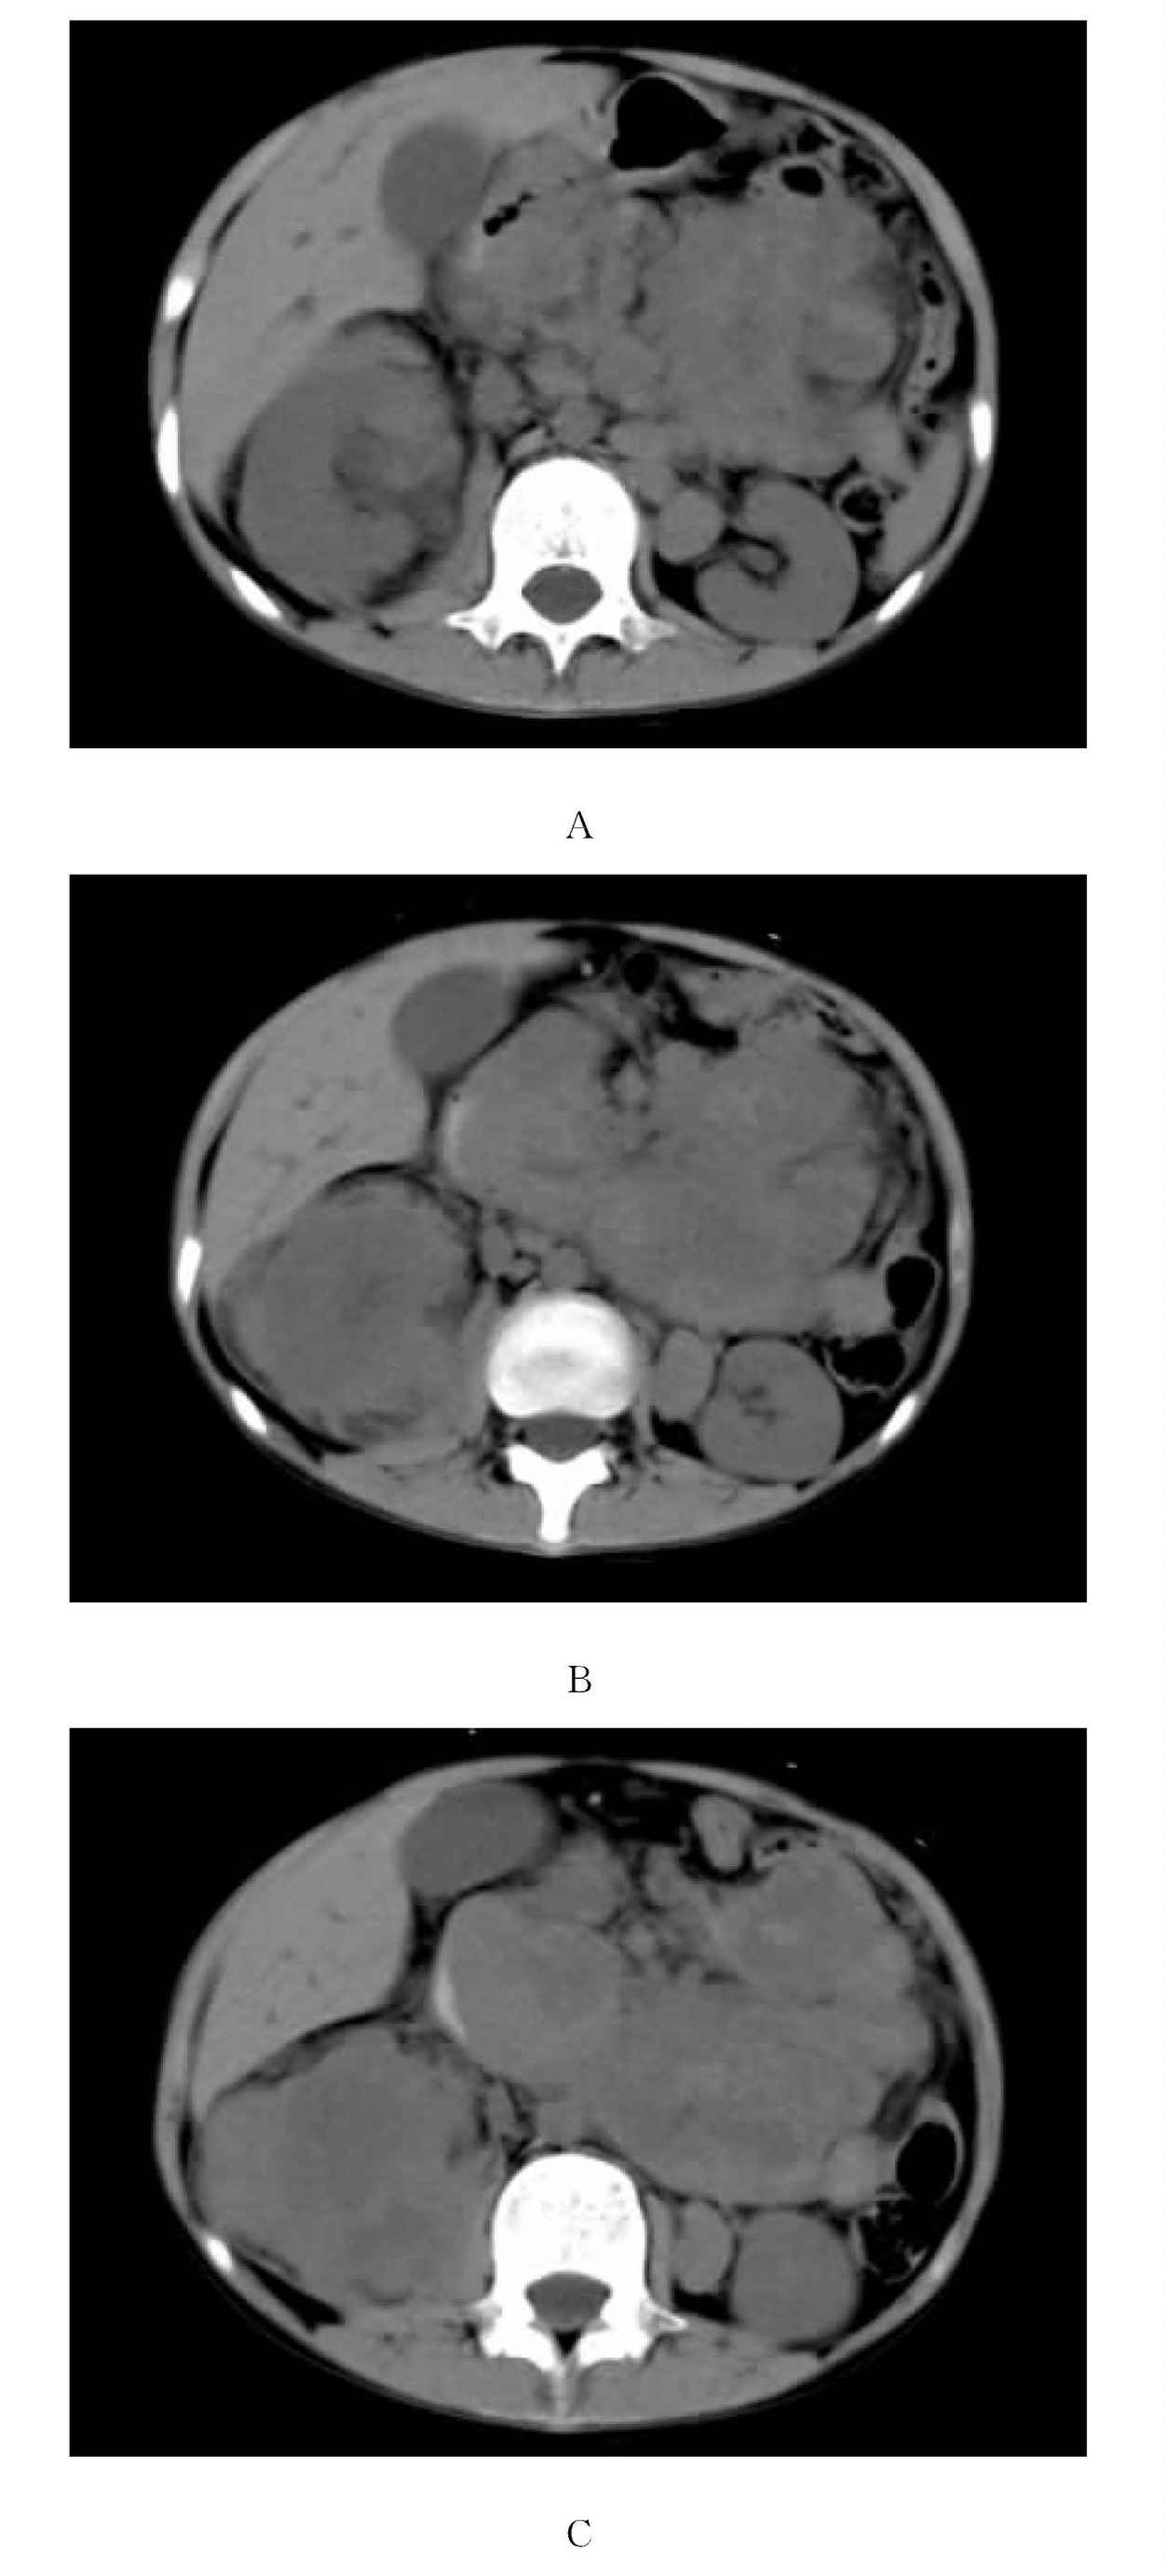
\includegraphics[width=.7\textwidth,height=\textheight,keepaspectratio]{./images/Image00341.jpg}
 \captionsetup{justification=centering}
 \caption{NHL侵及右肾\\{\small A~C为同一患者,右肾体积增大,密度不均,边缘毛糙;肾周间隙模糊。腹膜腔可见软组织肿块,腹膜后可见多个增大淋巴结}}
 \label{fig15-24}
  \end{figure} 

\subsection{肾转移瘤}

肾转移瘤并不少见,仅次于肝、肺、骨骼转移瘤。

\textbf{【病因病理】}
肾转移瘤的原发恶性肿瘤依次来源于肝、乳腺、肺、胃、子宫颈、结肠、胰腺等,亦有文献报道最常见于肺,并经尸检认为约19%的肺癌有肾转移,且多为双肾。

转移途径:①邻近结构恶性肿瘤的直接蔓延侵犯;②淋巴道转移;③血行转移;④对侧肾转移,常为癌栓经肾静脉侵入肾脏;⑤全身恶性肿瘤波及肾脏,如白血病、淋巴瘤等。

肾转移瘤常为多发和双侧性,少数为单侧,甚至为只有一个病灶。病灶多位于皮质,常在肾包膜下,但髓质也可有转移。瘤体呈球形、椭圆形或不规则形。大小多在1~2cm之间,但也有较大者。

\textbf{【临床表现】}
肾转移瘤多数体积较小,故很少因转移瘤发生肾功能的变化。肾脏受累症状常被其他脏器受累症状所掩盖。除原发癌的表现外,部分可有血尿、疼痛和肿块等。

\textbf{【CT表现】}
平扫多呈等或低密度灶,增强扫描因少血供轻度强化,仍呈低密度。病灶多数密度均匀、边缘光整。两肾多发小病灶,常见于肺、乳腺等肿瘤转移;单侧孤立性病灶,类似原发癌,多见于结肠癌转移;肾及肾周同时侵犯,多见于黑色素瘤转移。

\subsection{输尿管癌}

本病约占泌尿系肿瘤的1%~2%。

\textbf{【病理】}
多来自输尿管上皮组织。好发于输尿管中下段,多为单侧发病,偶为双侧。可以单发或多发。可孤立存在,或由肾盂肿瘤蔓延或种植形成,也可由膀胱肿瘤向上蔓延而来。绝大多数为移行上皮癌,鳞癌、腺癌和未分化癌均甚少见。肿瘤可呈广基浸润生长或呈菜花状生长,致不同程度的输尿管梗阻。早期局部淋巴结转移和血行转移到肺、肝和骨骼等并不少见。

\textbf{【临床表现】}
多发生于50岁以上,男性约为女性的2倍。主要症状为无痛性肉眼血尿,部分有腰痛,亦可出现腹部包块。晚期出现恶病质。

\textbf{【CT表现】}
平扫和增强可见病变部位输尿管管壁增厚、腔内软组织肿块、管腔狭窄和闭塞,以及肾盂肾盏积水表现(图\ref{fig15-25})。肿块小者多呈圆形,边缘较光整或有小棘状突起;肿块较大者(>5cm)则多不规则,中央可有坏死液化,周围有粘连浸润。增强扫描呈轻度不均匀强化,与管壁强化程度相仿;肾盂期可见输尿管内不规则充盈缺损。增强扫描还可明确邻近脏器的侵犯程度及有无淋巴结转移。

\begin{figure}[!htbp]
 \centering
 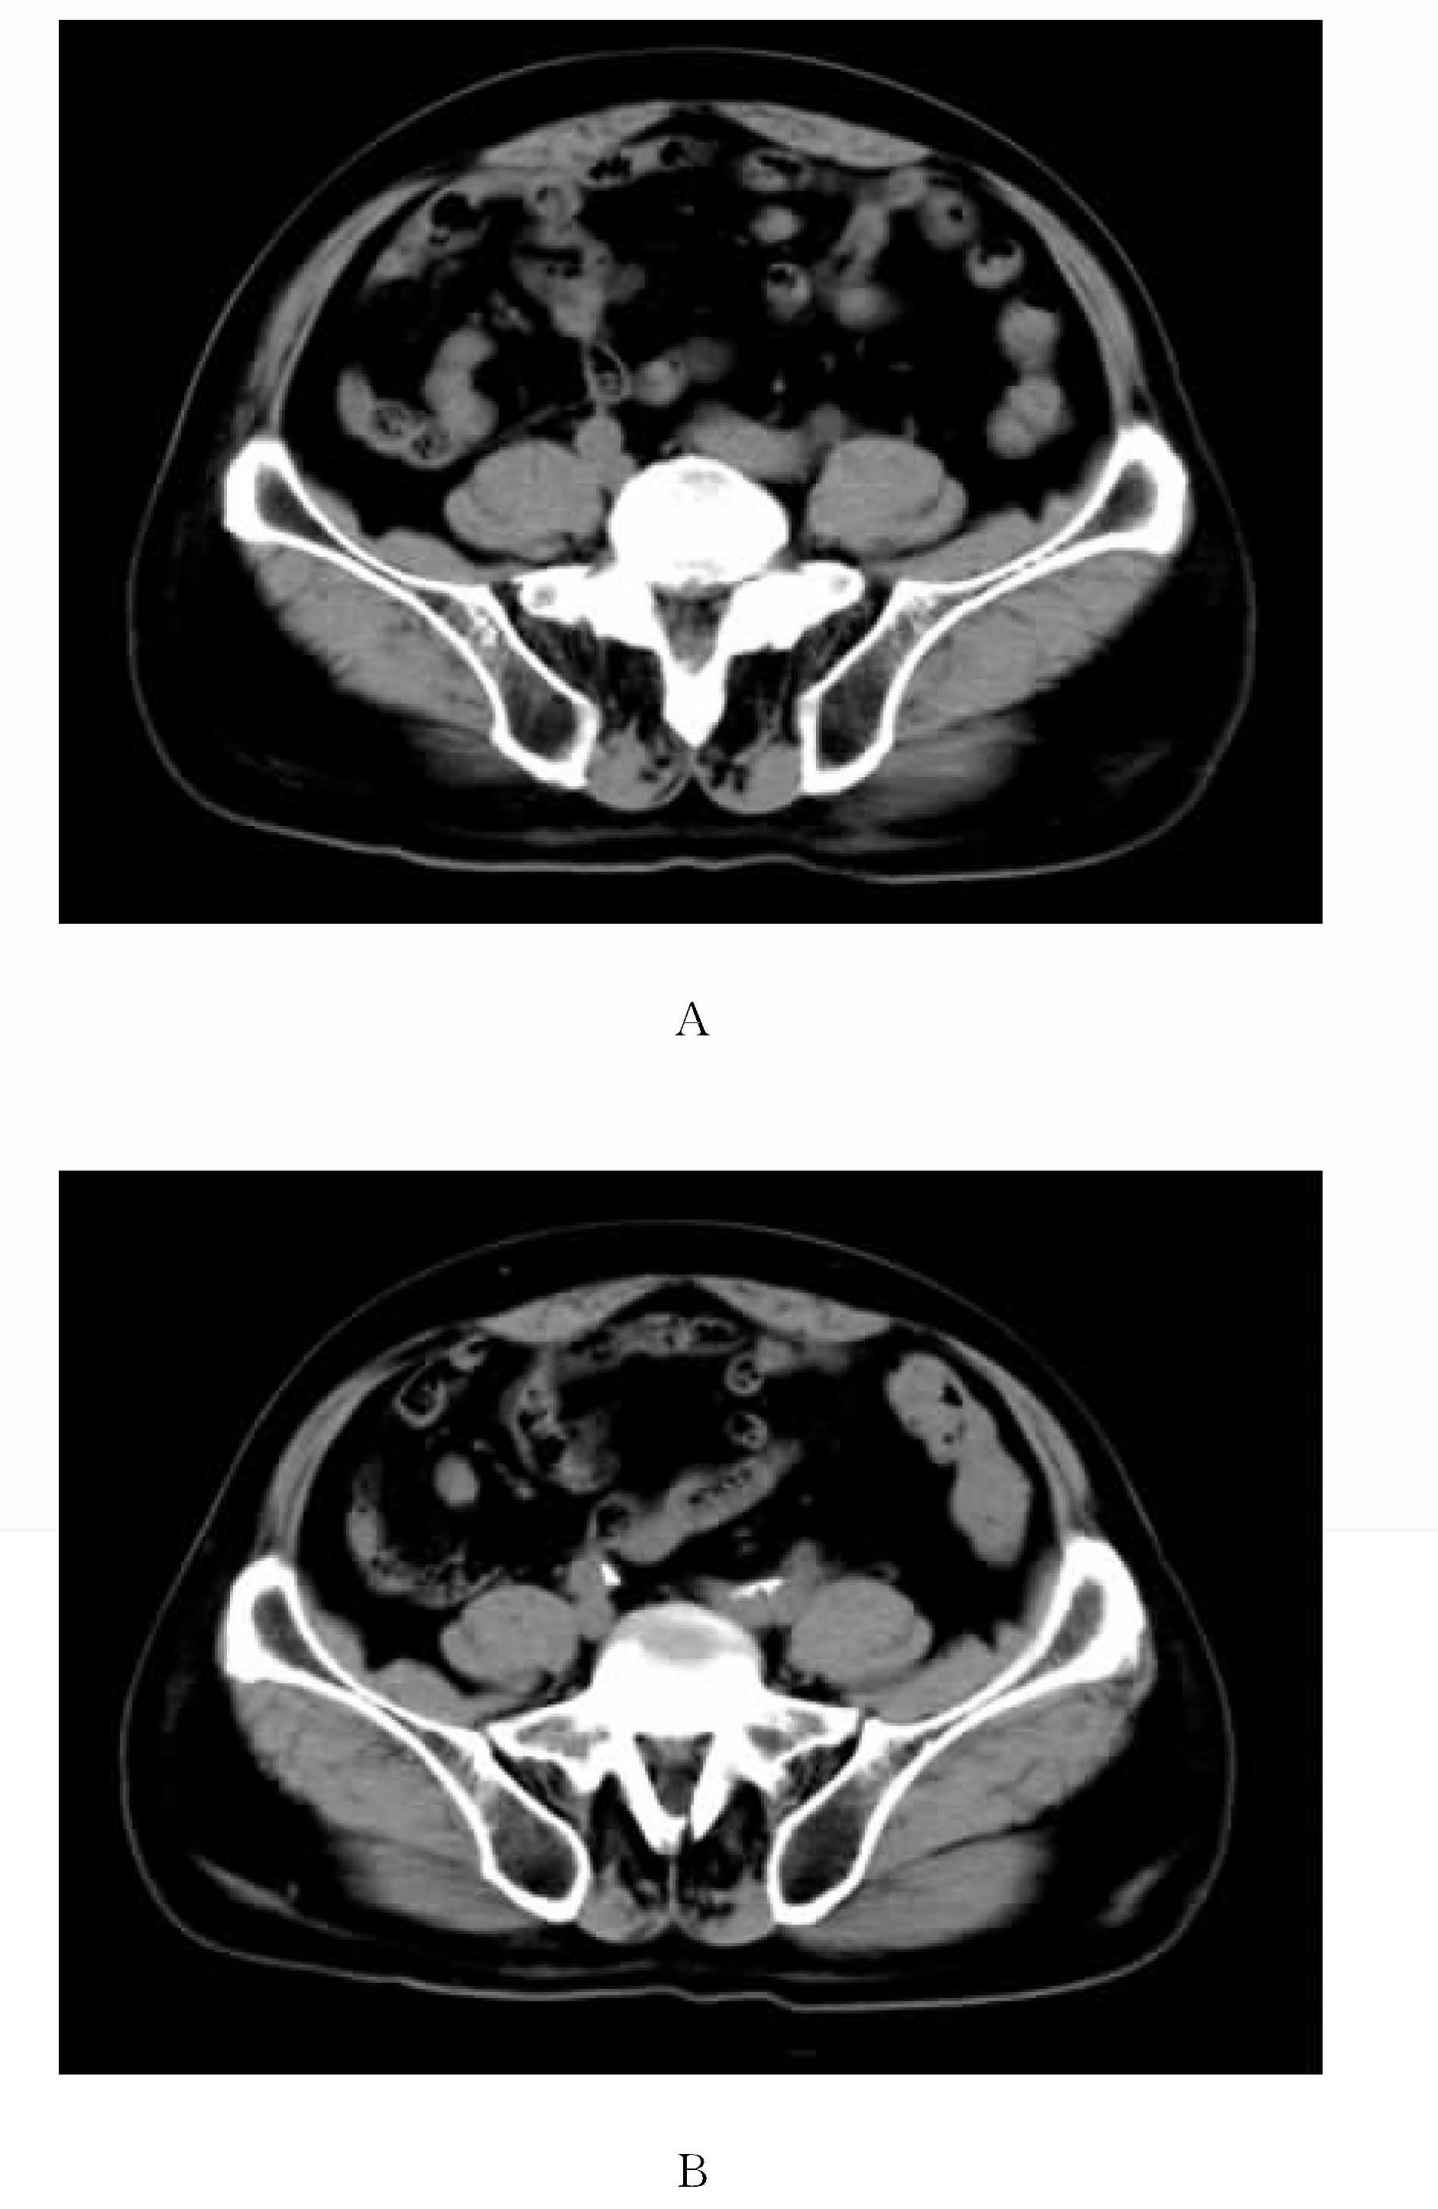
\includegraphics[width=.7\textwidth,height=\textheight,keepaspectratio]{./images/Image00342.jpg}
 \captionsetup{justification=centering}
 \caption{输尿管癌(乳头状移行细胞癌)\\{\small A、B为上下连续层面。A示左侧输尿管近第二狭窄处积水扩张;B示其下层面管腔截然变窄,局部输尿管不规则变形,管壁不规则增厚、边缘毛糙}}
 \label{fig15-25}
  \end{figure} 

\textbf{【鉴别诊断】}

1.结石:即使阴性结石其CT值亦明显高于肿瘤,但应注意输尿管肿瘤合并钙化或结石的比率较高。

2.血块:密度与形成时间长短有关,无强化表现。短期随访可有明显的退缩。

3.息肉:发病年龄小。好发于输尿管上1/3段。呈条状充缺,管壁光滑,无破坏。但严格说良、恶性肿瘤形态学无明显特异性,有赖于细胞学和病理组织学。

4.结核及其他炎性狭窄:一般病变范围较长,管壁呈均匀性增厚。结核则呈不规则串珠状的狭窄及扩张,均伴肾脏及膀胱的相应改变。

此外,还应与腹膜后纤维化及其他腹膜后占位性病变相鉴别。

\subsection{膀胱癌}

本病为泌尿系最常见的恶性肿瘤,约占所有恶性肿瘤的4%。

\textbf{【病理】}
最常见于膀胱三角区、侧壁和后壁,常为多中心。90%为移行细胞癌,腺癌约占2%,鳞癌约占5%~10%,鳞癌多发生于有慢性炎症的病人。此外,相当部分组织学上的良性乳头状瘤,性质上却是恶性的,因此乳头状瘤为潜在恶性肿瘤,甚至有人称为乳头状癌Ⅰ级。肿瘤为带蒂的乳头状肿块,或呈广基生长,也有溃疡和浸润型的。多向邻近组织直接蔓延,少数局部淋巴结转移和血行转移到肺、肝和骨骼等。

\textbf{【临床表现】}
好发于成年男性,40岁以上者占93%。主要为无痛性肉眼血尿,多为间歇出现的全程血尿。可有尿频、尿急和排尿困难。

\textbf{【CT表现】}
①腔内肿瘤:可以是单个或多个突入腔内(图\ref{fig15-26})。肿瘤密度欠均匀,边缘清晰,内可有斑点状钙化。增强扫描强化不显著。当累及黏膜下层或肌层时,表现膀胱壁增厚,但CT不能区别限于黏膜内或已侵入黏膜下层及肌层。晚期肿瘤可充满整个膀胱,如肿瘤位置接近输尿管的开口,可导致输尿管梗阻。②累及膀胱周围组织:累及浆膜层后,可见膀胱壁外缘不光滑、与周围的脂肪层分界模糊,甚至伴纤维条索状粘连。③累及邻近器官:可见膀胱精囊三角消失,前列腺、精囊增大变形等。④肿瘤蔓延达盆壁或有淋巴结转移:可累及前腹壁、盆壁及闭孔内肌等。盆腔淋巴结>15mm者为阳性。

\begin{figure}[!htbp]
 \centering
 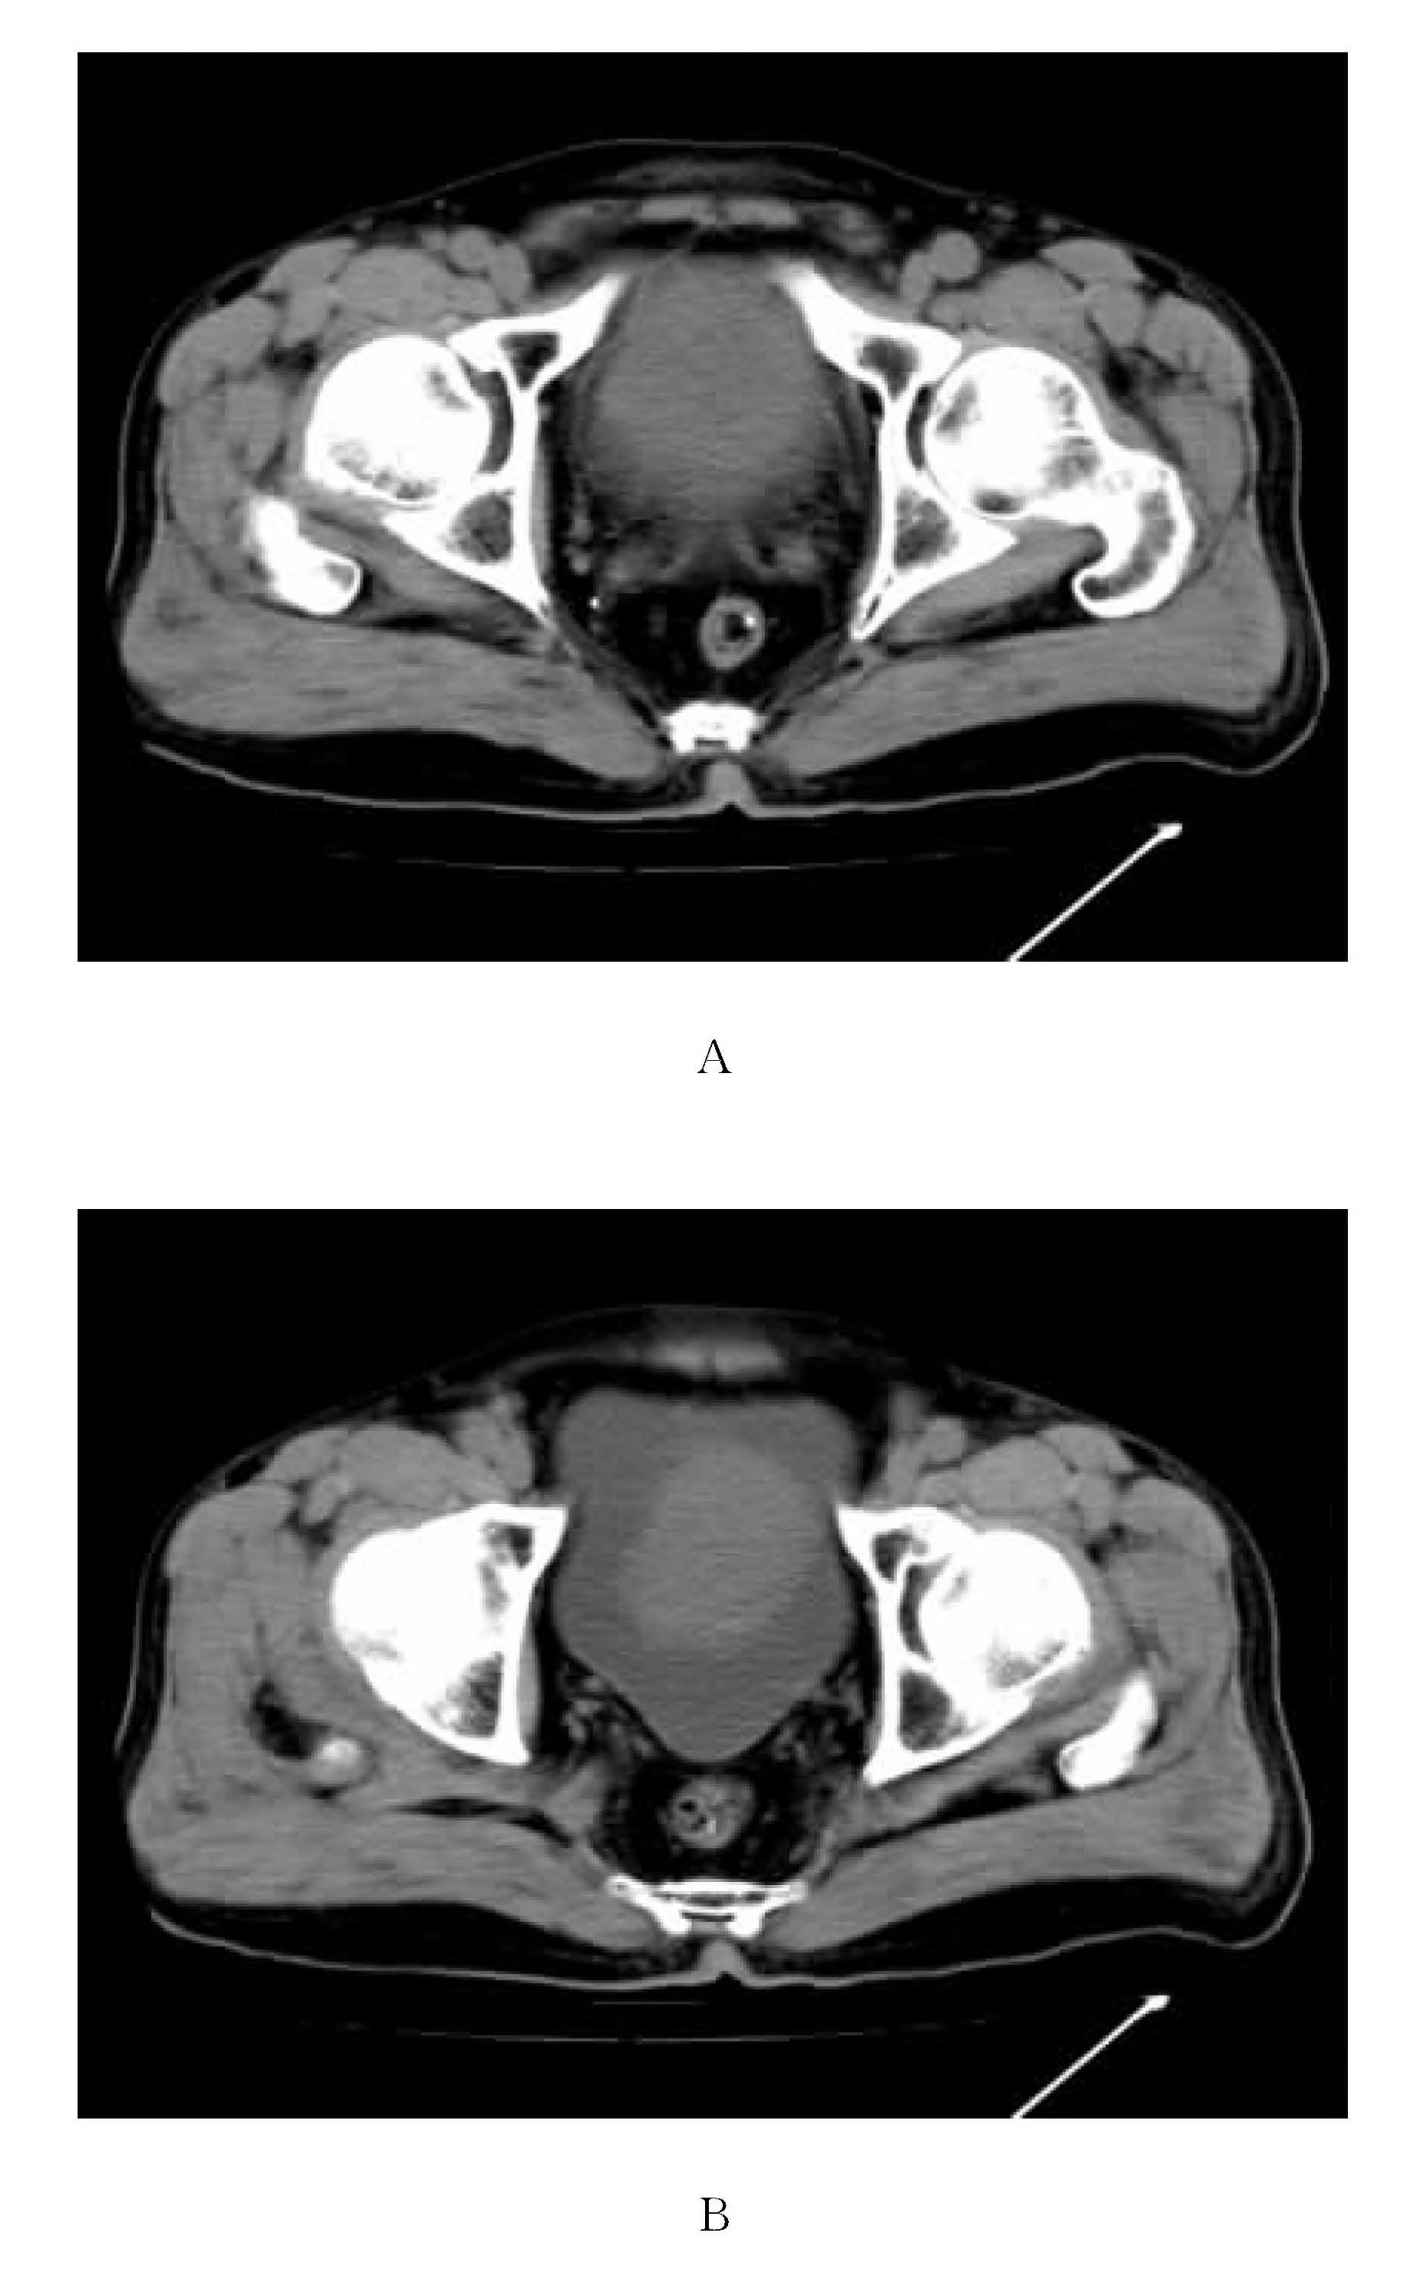
\includegraphics[width=.7\textwidth,height=\textheight,keepaspectratio]{./images/Image00343.jpg}
 \captionsetup{justification=centering}
 \caption{膀胱癌\\{\small A、B为同一患者,肿瘤由颈部向上生长(手术证实)}}
 \label{fig15-26}
  \end{figure} 

CT分型:国内有学者根据其病理分型,将CT表现分为4型:①乳头状有蒂型;②非乳头状有蒂型;③乳头状宽基底型;④非乳头状宽基底型。

\textbf{【鉴别诊断】}

1.其他类型膀胱肿瘤:如良性的乳头状瘤、炎性假瘤,恶性的肉瘤、淋巴瘤均表现为膀胱腔内的占位,CT难以鉴别。

2.膀胱结石:无论阳性或阴性其密度均明显高于膀胱癌等一般肿块,且位置有活动性。

3.血块:膀胱壁完整,无受侵;变换体位有活动性。

4.膀胱结核:膀胱多明显缩小,轮廓毛糙,即所谓“挛缩膀胱”;均伴肾脏、输尿管的相应改变。与肿瘤不难鉴别。

5.神经源性膀胱:膀胱多呈宝塔状,体积增大,小梁甚粗,膀胱壁普遍增厚。IVP多伴输尿管返流。

6.脐尿管肿瘤:膀胱前上方、壁外的软组织肿块,并侵犯膀胱顶部前方黏膜;而膀胱癌以腔内肿块及膀胱壁改变为主,壁外改变较少,且顶部前壁非好发部位。

7.前列腺增生和前列腺癌:突入膀胱内块影的上下径远小于横径,仅1~2个层面可显示。另外膀胱底部和侧壁正常,与块影可分开或紧贴。当然整个膀胱壁可因排尿障碍而广泛增厚,但无局部改变。

\subsection{脐尿管癌}

脐尿管源于尿囊上部,在胚胎第七周,膀胱处于脐部,随后沿前腹壁向下沉降,上部渐缩小、闭锁为脐尿管索,此处组织结构与膀胱相同。

\textbf{【病理】}
脐尿管癌少见,占膀胱肿瘤的0.17%~0.34%。发生于膀胱内或近膀胱的脐尿管端。其中黏液腺癌占95%。脐尿管上皮为移行上皮,而脐尿管肿瘤多为腺癌,对此有两种解释:一是移行上皮向柱状上皮的化生,进而恶变;二是腺癌起源于脐尿管内残余的岛状含黏液的后肠上皮。

\textbf{【临床表现】}
多见于40~70岁。早期多无症状,肿块较大或浸润膀胱壁时才出现临床症状。主要表现为腹痛和中下腹中轴线上腹内包块,当侵及膀胱时出现膀胱刺激征和血尿。

\textbf{【CT表现】}
位于膀胱顶部中轴线上软组织肿块或含钙化的囊性肿块;肿块主要位于膀胱外,推压膀胱,与膀胱壁界限不清,局部膀胱壁增厚。肿块内可有斑点状钙化,位于肿块中央或周围。增强扫描肿块强化程度不一,多强化明显。肿块前缘可侵及腹壁,还可直接侵犯或沿淋巴道转移至大网膜、腹膜、盆腔淋巴结及器官。

\textbf{【鉴别诊断】}
脐尿管囊肿有时可呈实性密度或因感染而壁厚,但囊肿壁相对均匀规则,其钙化粗大,沿壁呈环状;而癌变壁厚而不规则,钙化呈细小斑点状。

\section{肾血管病变及肾移植}

\subsection{肾静脉血栓}

本病少见,可发生于任何年龄,但在早产、产伤或先天性血管异常的婴儿较为常见。

\textbf{【病因】}
①肾病综合征:是成人肾静脉血栓形成最常见的病因,其机制为大量蛋白尿所致的有效血容量降低使血液处于高凝状态;肾实质水肿使压力增高导致肾静脉血流缓慢。②下腔静脉血栓形成向肾静脉蔓延。③妊娠合并肾静脉血栓形成,可能与子宫压迫有关。④儿童期胃肠炎症造成脱水状态。⑤高凝血状态。

\textbf{【临床表现】}
急性期有腰痛和上腹部疼痛,还可有寒颤、发热及感染休克症状,也可有血尿、脓尿和蛋白尿。双侧肾静脉栓塞可出现急性肾功能衰竭。肾病综合征是最常见的伴随症状。

\textbf{【CT表现】}
增强扫描肾静脉内低密度条状影或充盈缺损,为主要直接征象;肾皮髓质交界时间延长,还可见肾周静脉侧支循环形成。肾静脉近端增粗。肾影可增大,但如无急性肾梗死出现,通常在2个月后肾脏变小。在无功能的肾脏,肾静脉增粗可能是惟一表现,并可误诊为肾肿瘤。有时可见肾周或肾包膜下出血或积液。

\textbf{【鉴别诊断】}
①层流现象:见于增强早期,但不伴随静脉扩张,延迟重复扫描可排除假象。②肾静脉癌栓:亦形成静脉内充缺,但癌栓导致的静脉扩张限于病变之局部,且不规则。常合并腹膜后淋巴结增大,结合肾内等原发灶可予鉴别。

\subsection{肾梗死}

\textbf{【病因病理】}
肾动脉梗死的栓子常来源于心脏病如风湿性二尖瓣病变、心肌梗死、心房黏液瘤或主动脉瘤。此外,还可能与主动脉硬化、动脉瘤、外伤、休克、腹水、使用血管收缩剂等引起的阻塞有关。但部分病因不明。

急性肾动脉栓塞后,如完全栓塞而未能及时解除,则形成全肾性、部分性、节段性或多发性小的肾梗死。肾组织破坏、肾萎缩,最后产生纤维硬变。栓塞后血管坏死,一旦再通,即形成出血性梗死。

\textbf{【临床表现】}
取决于梗死的程度和范围,病人可有突发的剧烈腰痛和腹痛、低热、恶心、呕吐和白细胞升高、蛋白尿、血尿。1周后症状可缓解。少数后期出现高血压。肾动脉较小分支的梗死可无症状。

\textbf{【CT表现】}
平扫尤其是早期常无异常改变。增强扫描表现为边缘清晰的圆形或楔形低密度区。梗死灶大小与梗塞血管的大小成比例,通常大者可呈圆形,小者呈楔形。较大的病灶皮质缘可见环状的高密度强化带,即皮质边缘征,许多学者认为是梗死灶周围侧支循环(主要是包膜下血管)建立所致,这也是较大梗死灶在形态上呈圆形而非楔形的原因。肾梗死无占位效应。肾周极少受累,偶有肾旁筋膜增厚及肾周积液。后期病灶可瘢痕化,致皮质萎缩凹陷。

\textbf{【鉴别诊断】}
较大的梗死表现较典型,如特征性的皮质边缘征、结合临床不难鉴别。对较小的梗死灶应注意结合临床与局灶性肾盂肾炎、脓肿甚至肿瘤相鉴别。

\subsection{肾动脉狭窄}

肾动脉狭窄可为先天性或后天性。

\textbf{【病因病理】}
其病因主要为动脉粥样硬化、纤维肌肉增生(又称纤维肌发育不良,属血管纤维性病变。还可损害髂动脉、肠系膜上动脉和脑动脉),以及大动脉炎、神经纤维瘤、先天性肾动脉发育不良、肾动脉周围病变压迫等。

动脉硬化者病变常位于近肾动脉的开口处2cm一段,偶可累及远端及分支。纤维肌肉增生病变常位于中1/3和远1/3,常延及分支。先天性肾动脉发育不良常累及肾动脉主干或分支,受累肾动脉全段纤细,比一般肾动脉细1/2以上;管壁光滑,无狭窄后扩张;肾内动脉细小、稀少,肾脏常发育不良。

\textbf{【临床表现】}
青年发病常小于30岁,老年发病常大于50岁。有持续性高血压,肾区可闻及收缩期杂音。可伴有腰背痛或腹痛。动脉粥样硬化者可出现蛋白尿、血尿和管型尿、血尿素氮及肌酐升高、低血钾等。

\textbf{【CT表现】}
CTA可见肾动脉呈不同程度的狭窄。后天性(动脉硬化性)可有管壁钙化。晚期可见肾萎缩,实质普遍缩小,肾窦内脂肪增加;健侧代偿性增大(图\ref{fig15-27})。增强扫描或CTA可显示侧支循环的血管影。

\begin{figure}[!htbp]
 \centering
 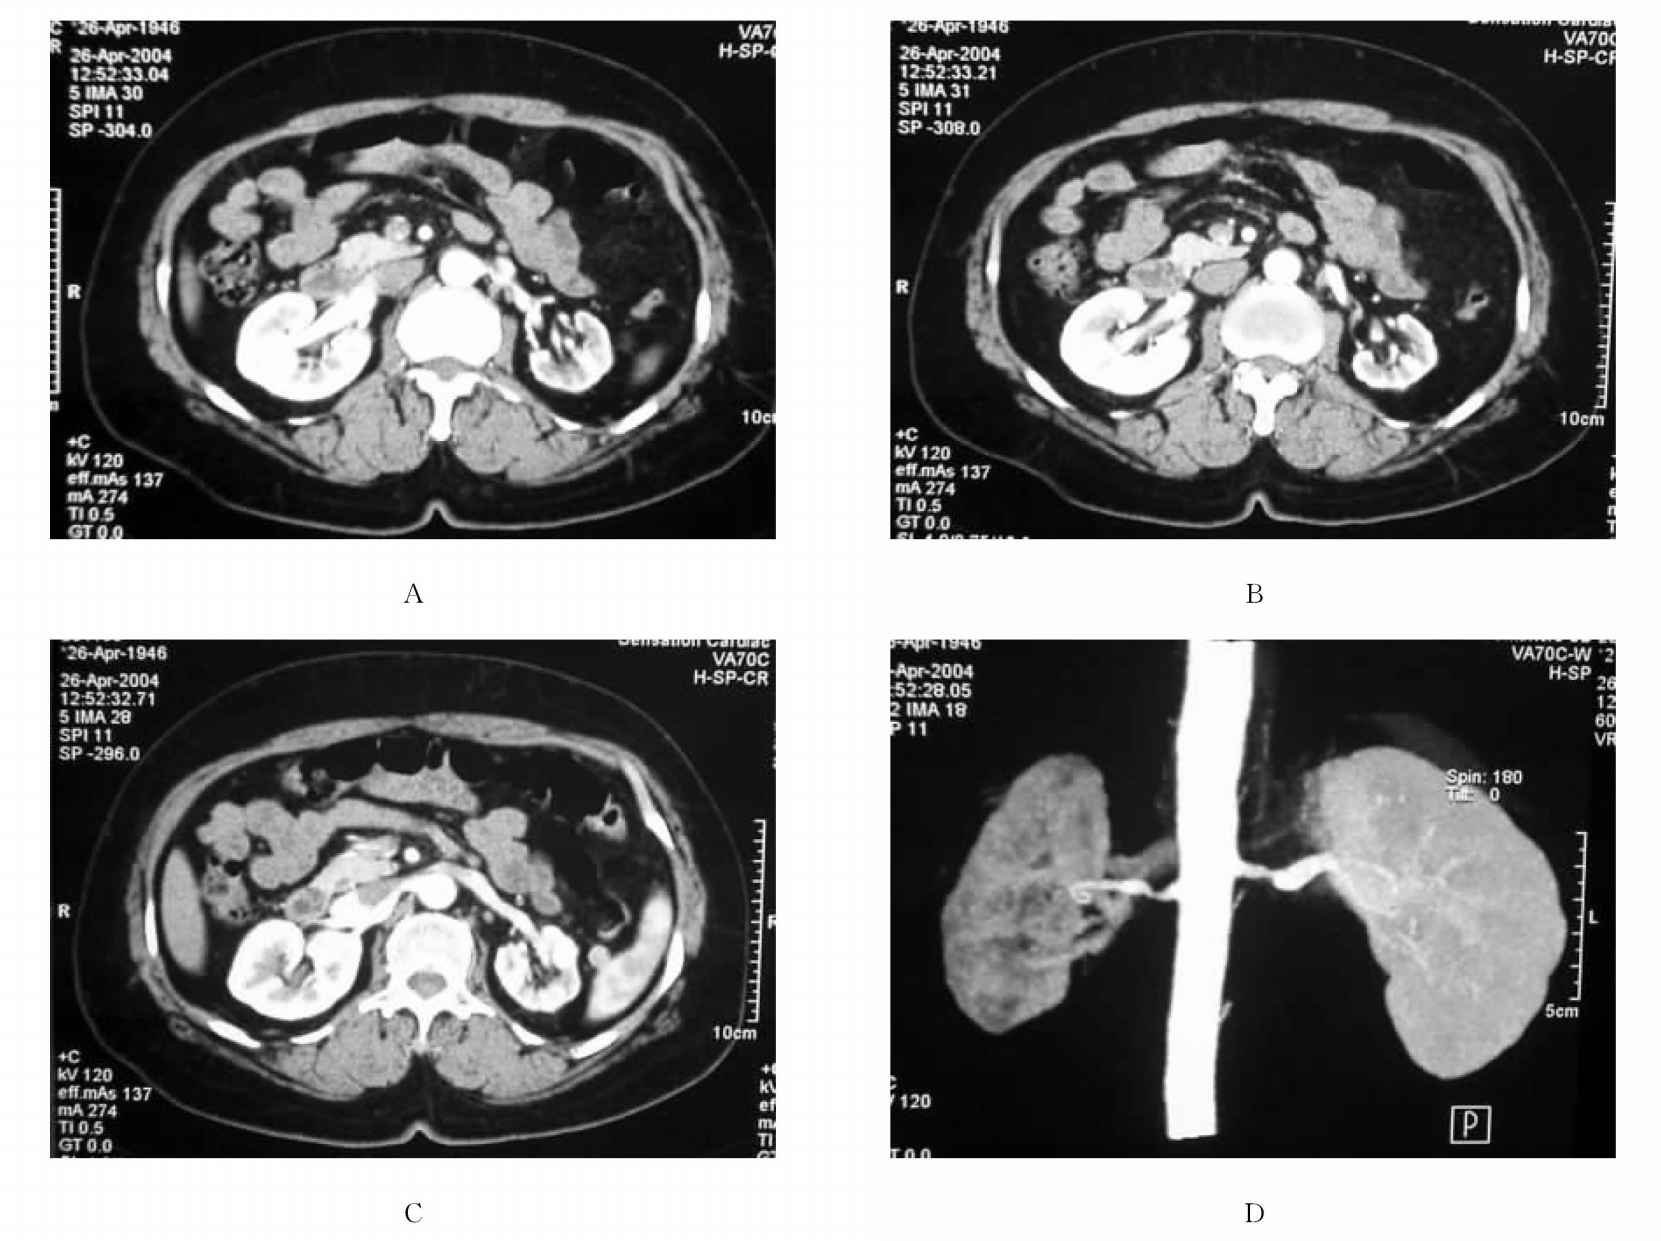
\includegraphics[width=.7\textwidth,height=\textheight,keepaspectratio]{./images/Image00344.jpg}
 \captionsetup{justification=centering}
 \caption{左肾动脉狭窄\\{\small A~D为同一患者,左肾动脉不规则狭窄,并发左肾萎缩}}
 \label{fig15-27}
  \end{figure} 

\subsection{肾动脉瘤}

本病亦可为先天性或后天性。

\textbf{【病因病理】}
其病因主要为动脉粥样硬化,其次是先天性肾动脉壁中层弹力纤维发育不良和外伤。偶见于细菌性动脉炎、结节性动脉外膜炎、梅毒、动脉脂肪变性等。约60%发生在肾动脉主干或第一肾动脉分叉处,约15%发生在肾实质内。约20%双侧发病。动脉瘤呈囊状或梭形,以前者常见,后者常伴肾动脉狭窄。25%动脉瘤囊壁有钙化。病变动脉供应的肾实质常发生缺血,还可同时存在动静脉瘘。

\textbf{【临床表现】}
一般无症状,但有时可有上腹痛、腰痛和血尿,局部可触及搏动性肿块或闻及杂音。由于动脉瘤压迫肾实质或降低血流引起肾素的增高,可出现高血压。

\textbf{【CT表现】}
平扫可见高密度的瘤体、瘤壁弧形或壳状钙化;增强扫描可见强化的瘤体及局限性肾缺血所致的楔形低密度区,但如瘤体内有血栓则可无明显强化或见到充盈缺损。CTA更有利于显示瘤体的位置、大小和形态。

\subsection{肾动静脉瘘}

本病可以是先天性的,亦可发生于肾手术后。可引起节段性肾缺血,从而产生高血压。

\textbf{【临床表现】} 主要为血尿、蛋白尿或高血压。局部可闻及杂音。

\textbf{【CT表现】}
增强扫描或CTA可显示肾动脉分支扩张、迂曲,尤其是通向病灶的肾动脉明显扩张,肾静脉早期显影,还可见局部缺血表现。晚期可有局限性肾萎缩表现。

\subsection{胡桃夹综合征}

本病又称左肾静脉压迫综合征或“胡桃夹”现象。属正常变异。

\textbf{【病因病理】}
左肾静脉行走于肠系膜上动脉与腹主动脉的夹角内,由于儿童发育上的特点和各种原因引起的内脏下垂均可导致左肾静脉受压变窄,而腹主动脉左侧的一段静脉扩张,犹如“干果钳”样改变。血液回流障碍致使左肾淤血增大,但不影响肾功能。随着年龄增长和内脏下垂的改善,可恢复至正常。

\textbf{【临床表现】}
可见于小儿及成人。可表现为无症状性、直立性蛋白尿或持续性肉眼血尿,血尿多在剧烈运动后或傍晚出现。

\textbf{【CT表现】}
72%的正常人CT可显示这一变异。左肾静脉在肠系膜上动脉与腹主动脉的夹角处管腔受压变窄,左肾静脉近端和远端宽度差别可达2倍以上,而这一水平的下腔静脉无相应扩张。左肾体积可略增大,其形态、密度多正常。有时可见肾静脉周围迂曲扩张的侧支静脉影。

注意不要与肾静脉内血栓或癌栓所致的肾静脉扩张相混淆。

\subsection{移植肾}

\subsubsection{正常移植肾}

\textbf{【病理】}
正常移植肾位于右侧或左侧髂窝内,通常仅上2/3部分覆盖腹膜。一般移植肾动脉与受体髂内动脉端端吻合或与髂外动脉端侧吻合,移植肾静脉与受体髂总静脉或与髂外静脉端侧吻合。

\textbf{【CT表现】}
移植肾常位于右髂窝,肾轴可以水平向或垂直向;正常移植肾轮廓光整、密度均匀、皮髓质分界清晰。平扫时CT值在30~40Hu之间,增强扫描后CT值在60~80Hu之间。动态增强CT扫描皮髓质交界时间在36~74秒之间,平均45.7秒。此外,移植肾与腰大肌的界限清晰,有时可与膀胱接触,造成膀胱压迹。

\subsubsection{肾移植术后的排异反应和并发症}

\textbf{【病理】}
排异反应是受体对移植肾抗原产生的一系列细胞和体液的免疫反应。并发症包括尿路梗阻、尿外渗、淋巴囊肿、肾周血肿,以及肾动脉狭窄和梗死等。

\textbf{【临床表现】}
肾移植后当病人出现发热、少尿或无尿、移植肾区疼痛等症状时,首先应考虑有排异反应可能,鉴别诊断主要是与移植肾术后并发症鉴别。

\textbf{【CT表现】}

1.排异反应:90%的病人可以发生。常分为4型:超急性、加速性、急性和慢性。①超急性和加速性:常在术后即刻或1~2天内发生。CT表现因肾内出血而显著增大、密度不均匀,如果持续时间长可发生肾脏破裂。②急性:常发生于术后1周内,少见于1~2天。CT表现无特征性,可见肾增大、密度降低、肾窦受压。③慢性:常发生于6~12个月之间。CT示移植肾大小正常或缩小,CT值增加;亦可体积增大,失去原肾形。增强扫描皮髓质分界不清、肾实质密度不均、肾轮廓高低不平、肾盂肾盏呈“多囊状”积水。

2.急性肾小管坏死:常由缺血所致,通常发生于移植后48h,多见于术后1周。CT表现无特征性,表现为肾脏肿大、皮髓质分界不清,增强扫描皮髓质交界时间可以正常也可以异常。结合临床,因肾小管坏死时消耗钠导致高尿钠,而排异反应时钠潴留导致低尿钠可予鉴别。

3.泌尿系统并发症:①尿路梗阻:发生率约5.5%。输尿管膀胱吻合口的水肿、狭窄,输尿管过长扭曲、粘连成角,输尿管被精索、血凝块、淋巴囊肿、脓肿和腹膜后纤维化组织压迫等均可造成梗阻。CT表现主要为积水。②肾周积液:发生率约50%。其原因为淋巴囊肿(与手术时淋巴管切断有关)、尿性囊肿、脓肿和血肿等。

4.血管系统并发症:发生率10%~16%。常见的是肾动脉狭窄,较少见的是肾静脉血栓、吻合口出血、动静脉瘘和假性动脉瘤。

5.移植术后肿瘤:与免疫抑制有关。以皮肤和唇的鳞癌,以及淋巴瘤较常见。

\protect\hypertarget{text00023.html}{}{}

